%! TEX root = thesis.tex
%! TEX TS-program = xelatex
\documentclass[12pt,twoside]{report}

%%%%%%%%%% PACKAGES  %%%%%%%%%5
\usepackage{amsmath}
\usepackage{amssymb}
\usepackage{braket}
\usepackage{graphicx}
\usepackage{caption}
\usepackage{cite}
\usepackage{kantlipsum}
\usepackage{bibentry}
\usepackage{sectsty}
\usepackage{hyperref}
% \usepackage{refcheck} %% checks whether all figures have been referred to
\usepackage[margin=2.5cm,bottom=3.5cm]{geometry}
\graphicspath{{frontmatter}{introduction}{methods}{metalsRG}{ESIAM}{tileForm}{tileESIAM}{tileHF}{conclusions}{appendices}}

%%%%%%%%% HEADER AND FOOTER
\usepackage[dvipsnames]{xcolor}
\usepackage{fancyhdr}
\usepackage[fit]{truncate}
\definecolor{link}{rgb}{0.6, 0.3, 0.0}
\pagestyle{fancy}
\renewcommand{\chaptermark}[1]{ \markboth{#1}{} }
\renewcommand{\sectionmark}[1]{ \markright{#1}{} }
\fancyhead{}
\renewcommand{\headrulewidth}{1pt}
\renewcommand{\footrulewidth}{1pt}
\renewcommand{\headrule}{\hbox to\headwidth{%
  \color{darkgray}\leaders\hrule height \headrulewidth\hfill}}
\setlength{\headheight}{25pt}
\fancyhead[LE]{\nouppercase{\hfill\color{Blue}\bf\truncate{400pt}{\rightmark}}}
\fancyhead[RO]{{\color{Blue}\bf\truncate{400pt}{\scshape\leftmark}\hfill}}
\fancyfoot[C]{\\\color{Blue}\bf\hfill\thepage\hfill}
\fancyfoot[L]{\\\color{Blue}\bf Abhirup Mukherjee\hfill}
\fancyfoot[R]{\\\color{Blue}\bf \hfill IISER Kolkata}
\fancypagestyle{plain}{
    \fancyhf{}
    \renewcommand{\headrulewidth}{0pt}
    \renewcommand{\footrulewidth}{1pt}

    \fancyfoot[C]{\color{Blue}\bfseries\thepage}
    \fancyfoot[L]{\color{Blue}\bfseries Abhirup Mukherjee}
    \fancyfoot[R]{\color{Blue}\bfseries IISER Kolkata}
}
%%%%%%% FONTS SETUP
\usepackage[T1]{fontenc}
\usepackage{lmodern}
\usepackage{fontspec}
\usepackage{bm}
\usepackage{newtxtext}
\usepackage{newtxmath}
\setcounter{tocdepth}{1}

%%%%%%% CUSTOM COMMANDS
\newcommand\blankpage{%
    \null%
    \thispagestyle{empty}%
    % \addtocounter{page}{-1}%
    \newpage}
\newcommand{\inpar}[1]{\paragraph{\it\textbf{{\color{Blue}#1}~}}~}
\numberwithin{equation}{section}
\renewcommand\theequation{{\color{Blue}\bf\arabic{section}.\arabic{equation}}}


%%%%%%%%%%% LINK COLORS
\hypersetup{
    colorlinks=true,
    linkcolor=link,
    filecolor=magenta,      
    citecolor=gray,
    pdftitle={Thesis: Abhirup Mukherjee},
    }

%%%%%%% FIGURES
\usepackage[format=plain,font=it,labelfont=bf]{caption}

\newcommand{\chapA}{Introduction}
\newcommand{\chapB}{Methods and Preliminaries}
\newcommand{\chapC}{Kondo Frustration via Charge Fluctuations: A Route to Mott Localisation in Infinite Dimensions}
\newcommand{\chapD}{A New Auxiliary Model Approach for Interacting Electrons: Mapping Impurity Models To Lattice Models}
\newcommand{\chapE}{Mott Criticality as the Confinement Transition of of a Pseudogap-Mott Metal: Insights on Mott Transition and Pseudogap in Two Dimensions}
\newcommand{\chapF}{Competing tendencies In Heavy Fermion Systems: Kondo screening vs. Mott localisation}
\newcommand{\chapG}{Holography of Entanglement in 2D Free Fermions: Emergent Geometry and Fermionic Criticality}
\newcommand{\chapH}{Summary, Conclusions and Future Work}

\begin{document}

% %! TEX root = thesis.tex
\begin{center}
\thispagestyle{empty}
\rule{\textwidth}{1mm}\\[0.5em]
\LARGE{\bf A New Auxiliary Model Approach To Fermionic Criticality: Insights on Mottness in Strongly Correlated Systems}\\[-0.2em]
\rule{\textwidth}{1mm}\\[1em]
\large{\it A thesis submitted in partial fulfilment\\ for the requirements of the degree of}\\[0.6em]
\Large{\bf Doctor of Philosophy}\\[0.6em]
{\it by}\\[0.6em]
\LARGE{\bf ABHIRUP MUKHERJEE}\\
\Large{(18IP014)}\\[0.6em]
\large{\it under the supervision of}\\[0.6em]
\Large{\bf Prof. Siddhartha Lal}\\[0.6em]
\large{\it to the}\\[0.6em]
\Large{Department of Physical Sciences,}\\
\Large{\bf Indian Institute of Science Education and Research Kolkata}\\[0.6em]
\Large{\it May, 2026}\\[0.6em]

\includegraphics[width=4cm]{iiserlogo.png}
\end{center}

% %! TEX root = thesis.tex
\chapter*{Declaration By The Student}

{\it Date: May 11, 2026}\\


\vspace{1em}
I, Mr. {\bf Abhirup Mukherjee}, Roll. No. 18IP014, dated May 11 2026, a student of the Department of Physical Sciences of the Integrated PhD Programme of IISER Kolkata, hereby declare that this thesis is my own work and, to the best of my knowledge, it neither contains materials previously published or written by any other person, nor has it been submitted for any degree/diploma or any other academic award anywhere before. I have used the originality checking service to prevent
inappropriate copying. 

I also declare that all copyrighted material incorporated into this thesis is in compliance with the Indian Copyright Act, 1957 (amended in 2012) and that I have received written permission from the copyright owners for my use of their work. I hereby grant permission to IISER Kolkata to store the thesis in a database which can be accessed by others. 

\vspace{1em}
\begin{flushleft}
\begin{minipage}{0.11\textwidth}
Signature:
\end{minipage}
\begin{minipage}{0.3\textwidth}

\includegraphics[width=\textwidth]{signature.png}
\end{minipage}
\vspace{1em}

Name: ABHIRUP MUKHERJEE
\vspace{1em}

Department of Physical Sciences

Indian Institute of Science Education and Research Kolkata

Mohanpur 741246, West Bengal, India
\end{flushleft}

% %! TEX root = thesis.tex
\clearpage
\chapter*{Certificate From The Supervisor}

{\it Date: May 11, 2026}\\

\vspace{1em}
This is to certify that the thesis titled "A New Auxiliary Model Approach To Fermionic Criticality:Insights on Mottness in Strongly Correlated Systems" submitted by Mr. {\bf Abhirup Mukherjee}, Roll. No. 18IP014, a student of the Department Physical Sciences of the Integrated PhD Programme of IISER Kolkata, dated May 11 2026, is based upon his own research work under my supervision. I also certify, to the best of my knowledge, that neither the thesis nor any part of it has been submitted for any degree/diploma or any other academic award anywhere before. In my opinion, the thesis fulfils the requirement for the award of the degree of Doctor of Philosophy.

\vspace{0.5em}
\begin{flushleft}
\begin{minipage}{0.11\textwidth}
Signature:
\end{minipage}
\begin{minipage}{0.3\textwidth}
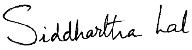
\includegraphics[width=\textwidth]{siddharthaSign.png}
\vspace*{0.4em}
\end{minipage}
\vspace{1em}

Name: Prof. Siddhartha Lal
\vspace{1em}

Professor

Department of Physical Sciences

Indian Institute of Science Education and Research Kolkata

Mohanpur 741246, West Bengal, India
\end{flushleft}

% %! TEX root = thesis.tex
\clearpage
\blankpage

\thispagestyle{plain}
\vspace*{200pt}
\begin{center}
{\it \Large From You, 5 Years Ago}
\end{center}

% %! TEX root = thesis.tex
\chapter*{Acknowledgements}

The journey of a PhD is a long endeavour, and I have had the fortune of benefiting from the help and support of many people.
\vspace{1em}

My first note of thanks goes to my supervisor, for helping me, as he often puts it, upgrade from version 1.0 to version 2.0 over the span of five years. Working with him has shaped and matured not only my ideas about how to carry out research, but also my understanding of how best to mentor others.
\vspace{1em}

I have also benefited a lot from interacting with my predecessors Anirban da and Siddhartha da as well as my present group members Debraj, Arnabesh, Sukalyan, Sourav da, Harsha and Ranbir. I am grateful to each of them for the many things I have learnt through our discussions.
\vspace{1em}

My collaborators outside the group have often shared valuable feedback on my work, and provided opportunities to venture outside my usual domain of research. In this regard, I am very thankful to Aashish, Anjan, Prof. A Taraphder, Prof. N S Vidhyadhiraja, Prof. S. R. Hassan, Prof. A Mukherjee, Prof. K Natarajan and Prof. S Pujari.
\vspace{1em}

Thanks are also due to my research progress committee members, Prof. Anandamohan Ghosh and Prof. Ritesh Singh, for ensuring my doctoral work stays on track and for providing regular reviews that often improved the quality of my research.
\vspace{1em}

I would also like to thank IISER Kolkata, SERB (Government of India), and the National Supercomputing Mission for supporting my research and enabling my participation in domestic and international conferences through multiple funding channels.
\vspace{1em}

It's important to have good friends that can support you through difficult periods of your life. I am really blessed in this regard. My friends back home -- Shrabona and Anurag -- as well as my friends at IISER Kolkata -- Biswajit, Debabrata, Sowrabh, Kaustubh, Gourab and Sushrat, among many others, are relations that I deeply value.
\vspace{1em}

Most importantly, I would like to thank my wonderful family -- my parents and my {\it dada} and {\it boudi} -- for having faith in me and for supporting my dreams in every way possible. This thesis is dedicated to my {\it dimma} -- my maternal grandmother -- who passed away during the third year of my PhD. She was a woman of remarkable mental fortitude and wisdom, and I have always tried to emulate the dedication she put into everything she did.

% %! TEX root = thesis.tex
\chapter*{List Of Publications}

\begin{itemize}
	\item[1.] {\it Mott Criticality as the Confinement Transition of a Pseudogap-Mott Metal}. {\bf Abhirup Mukherjee}, S R. Hassan, A Mukherjee, N S. Vidhyadhiraja, A Taraphder, S Lal. {\bf New J. Phys. 28 013503} (2026)
	\item[2.] {\it Holographic entanglement renormalisation for fermionic quantum
matter.}. {\bf Abhirup Mukherjee}, S Patra, S Lal. {\bf J. Phys. A: Math. Theor. 57 275401} (2024)
	\item[3.] {\it Mott Criticality as the Confinement Transition of a Pseudogap-Mott Metal}. {\bf Abhirup Mukherjee}, S R. Hassan, A Mukherjee, N S. Vidhyadhiraja, A Taraphder, S Lal. {\bf New J. Phys. 28 013503} (2026)
	\item[4.] {\it Mott Criticality as the Confinement Transition of a Pseudogap-Mott Metal}. {\bf Abhirup Mukherjee}, S R. Hassan, A Mukherjee, N S. Vidhyadhiraja, A Taraphder, S Lal. {\bf New J. Phys. 28 013503} (2026)
	\item[1.] {\it Mott Criticality as the Confinement Transition of a Pseudogap-Mott Metal}. {\bf Abhirup Mukherjee}, S R. Hassan, A Mukherjee, N S. Vidhyadhiraja, A Taraphder, S Lal. {\bf New J. Phys. 28 013503} (2026)
\end{itemize}


% \include{frontmatter/abstract.tex}
{\hypersetup{linkcolor=black}
% or \hypersetup{linkcolor=black}, if the colorlinks=true option of hyperref is used
\tableofcontents
}
% %! TEX root = thesis.tex
\chapter{Introduction: Mott Transitions and Kondo Breakdown}\label{sec:Introduction}
The rich physics of Mott metal-insulator transitions in strongly correlated systems has been an active subject of study for quite some time~\cite{hubbard1963electron,Mott_RMP_1968,milligan_1985,imada1998metal}. Their appearance in various materials such as the nickelates, cuprates, iridates and manganites, among others, is marked by complex phase diagrams that display dramatic changes in properties across changes in filling and/or bandwidth, even at low temperatures. 
The physics of Mott transitions is driven by the competition between two energy scales in the system: (i) the scale of itineracy, quantified by the bandwidth, and (ii) the scale of electron-electron repulsion. A Mott insulator arises when the electronic correlations are strong enough that low-energy electronic excitations become gapped, and the metallic valence band gets split into lower and upper bands; for an initially half-filled valence band, the lower band is filled at \(T=0\) while the upper band is vacant. Because of strong electronic repulsion, the electrons in the lower band form local moments which can show a variety of behaviour. This includes various symmetry-broken ground states such as an antiferromagnet~\cite{Lee_RMP_2006}, or symmetry-preserved states such as quantum spin liquids~\cite{Pustogow2018}. The physics of Mottness is also responsible for several very interesting phenomena, such as high-temperature superconductivity~\cite{Lee_RMP_2006}, non-Fermi liquids~\cite{Stewart2001RMP} and the various phases in magic-angle twisted bilayer graphene~\cite{Cao2018Mott,Cao2018}.

\begin{figure}[!htpb]
	\centering
	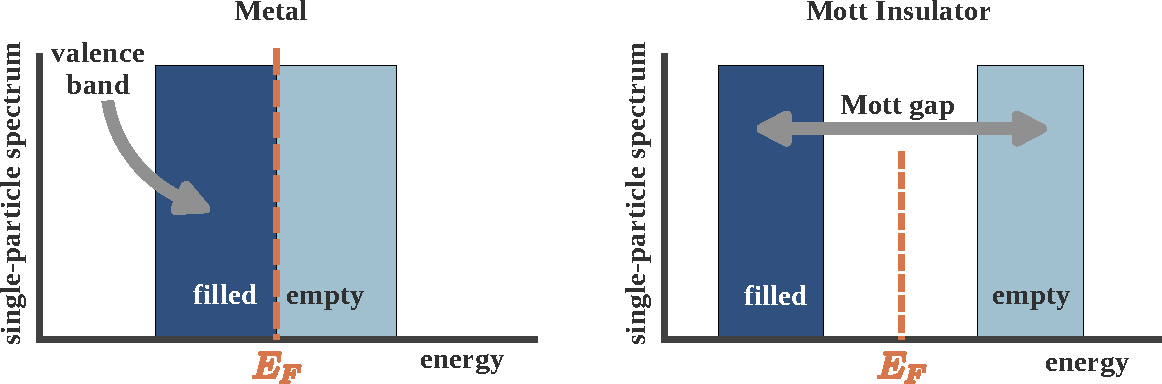
\includegraphics[width=\textwidth]{mottInsulator.pdf}
	\caption{}
	\label{mottInsulator}
\end{figure}

\section{Metal-insulator transition arising from strong correlation}
Initial attempts at explaining metal-insulator transitions was based on a non-interacting picture of electrons (through the work of Bethe, Sommerfeld, Bloch and Wilson among others); in such a picture, electronic bands can arise only from the scattering of electrons off the periodic lattice potential. One then distinguishes between metals and insulators at zero temperature by the position of the Fermi level \(E_F\) with respect to the bands: if \(E_F\) lies within a band gap, an integer number of bands will be completely filled and the system will be an insulator, whereas if \(E_F\) lies within one of the bands, the system will be a metal because there are vacant gapless excitations within the band. 

It was first pointed out by Boer and Verwey~\cite{Boer_1937} that certain insulators and semiconductors (such as nickel oxides) have a particle filling that, purely from band theory, would lead to partially filled bands. This poses a challenge because a partially filled band necessarily leads to a metallic phase (see Fig.~\ref{mottInsulator} (left)). The insulating behaviour of these materials therefore signals a fundamental limitation of single-particle band theory and points to a qualitatively different mechanism for electron localization---one driven by strong electron–electron interactions rather than by scattering from the lattice potential alone. This realization led to the concept of a Mott insulator, in which charge localization emerges as a genuine many-body effect despite the absence of a band gap in the non-interacting electronic structure. A very simple mechanism for this was put forth by Mott~\cite{Mott_1949,Mott1956,Mott961}: in the presence of a large local Coulomb repulsion cost \(U\) on a lattice site, the quantum states \(\ket{\Psi_1}\) in which the site is singly occupied get separated in energy from the states \(\ket{\Psi_2}\) where the site is doubly occupied by a gap of size \(U\); the former class of states \(\ket{\Psi_1}\) form the lower band (LB) while the latter \(\ket{\Psi_2}\) form the upper band (UB). If we now have a half-filled system (one electron per site), this electron will completely fill LB and leave UB vacant, leading to an insulating state (see Fig.~\ref{mottInsulator} (right)).

Given the above discussion, it is clear that a Mott insulator must involve a gap to charge excitations (excitations that add or remove an electron). It does not however determine the fate of the spin, orbital or other degrees of freedom. One scenario is when the spin or orbital degree of freedom undergoes spontaneous symmetry breaking into an ordered state; in the case of spin, this usually results in a superexchange interaction being generated and leads to an long-range ordered antiferromagnetic Neel state coexisting with the Mott state. Examples of such systems include vanadium sesquioxide V$_2$O$_3$ and its derivatives and the high-\(T_c\) cuprates (such as La$_2$CuO$_4$)~\cite{imada1998metal}. The other scenario is one where the spin degree of freedom retains its symmetry, and we end up with a quantum mechanically non-trivial entangled state (in order to quench the entropy). Examples of such states include quantum spin liquids~\cite{Isono2016}. Mott insulators without long-range order are of particular interest because of the possibility of topological order, fractional excitations, and novel metallic parent states.

A prototypical model for gaining theoretical understanding of Mott metal-insulator transitions on a lattice is the single-band Hubbard model~\cite{Anderson1959,hubbard1963electron,kanamori_1963,gutzwiller_1963}
\begin{equation}\begin{aligned}\label{hubbardModel}
	H = -t\sum_{\langle i,j \rangle , \sigma}(c^\dagger_{i,\sigma}c_{j,\sigma} + \text{h.c.}) - \frac{U}{2}\sum_i (n_{i, \uparrow} - n_{i, \downarrow})^2 - \mu N~.
\end{aligned}\end{equation}
The first term incorporates nearest-neighbour hopping on the lattice, while the second term introduces inter-electron repulsion when two electrons site on the same lattice site; in this way, the model incorporates the two competing tendencies of delocalisation and localisation that are responsible for the Mott MIT. The third term fixes the chemical potential and determines the filling of the lattice. Many of the materials that are studied for Mott MIT involve \(d-\)electrons that are five-fold degenerate, and these orbitals can hybridisation with ligand atoms. The Hubbard model avoids these complexities by focusing on only a single band that lies closest to the Fermi energy, and it is the states of this band that are described by the Hubbard model.

This leaves us with two channels for observing Mott MIT~\cite{imada1998metal}: (i) tuning the bandwidth, and (ii) tuning the filling. The former can be done, in experiments, by applying pressure. Filling is tuned by doping specific elements of a compound with elements of a different valence. The former is referred to as bandwidth-control metal-insulator transition, while the latter is called filling-control metal-insulator transition.

\section{Features of Mott metal-insulator transition}
\paragraph{Two complementary pictures of the Mott transition: Brinkman-Rice vs Mott-Hubbard.} Initial insights into the Mott MIT were obtained by Hubbard~\cite{hubbard1963electron}, thinking along lines similar to Mott. Within this picture, one starts from the insulating large \(U\) limit of the Hubbard model (eq.~\ref{hubbardModel}) (\(U \gg t\). We stay at half-filling for simplicity (\(\mu = 0\)). The large on-site repulsion leads to the formation of two bands at each site, the lower Hubbard band (LHB) associated with singly-occupied  states and the upper Hubbard band (UHB) associated with doubles and holes (states that incur a cost \(U\)). In the large \(U\) limit, these bands are well-separated, and the dynamics within the bands is a result of the motion of tightly bound holons and doubles (more on this later) that are generated because of the small but non-zero hopping probablity \(t\). As \(U/t\) is lowered, the bands come closer and a metal-insulator transition occurs at the critical value of \(U\) at which the gap vanishes. For lower \(U/t\), the bands overlap and we get a metal. This picture fails to provide an accurate description of the metal resulting from the melting of such a Mott insulator~\cite{georges1996}.

An alternative approach to the Mott MIT is due to Brinkman and Rice~\cite{brinkman_rice_1970}, where the authors applied Gutzwiller's variational method~\cite{Gutzwiller1965} to the half-filled Hubbard model. Gutzwiller's approach involves modifying, through variational factors, the hopping matrix elements that start from doubly occupied states, in order to reflect the electronic correlation at each site. By requiring that the number of doubly-occupied states vanish in the Mott insulating ground state, they obtained a critical value of the interaction strength. In the Brinkman-Rice scenario, therefore, the transition from the metal to the insulating phase occurs when the hopping matrix elements from the doubly-occupied to the singly-occupied states strictly vanishes. Note that in contrast to the Mott-Hubbard picture, this approach starts from a correlated Fermi liquid (renormalised due to the Gutzwiller factors). While it gives a better low-energy description of the correlated metal compared to the Mott-Hubbard picture, it fails to account for the high-energy physics, and treats the Mott insulator as a direct product state of local moments at each state (on account of the strictly zero hopping). This of course means that this method cannot explain antiferromagnetic superexchange processes in the Mott insulator~\cite{georges1996}.

\begin{figure}[!t]
	\centering
	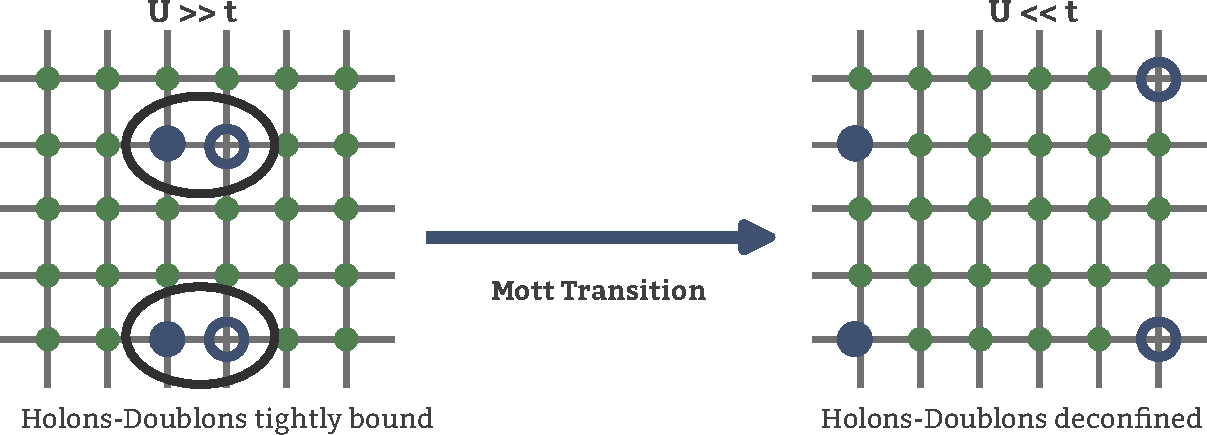
\includegraphics[width=\textwidth]{mottPicture.pdf}
	\caption{}
	\label{mottInsulator}
\end{figure}

\paragraph{Holon-doublon unbinding picture of the Mott MIT.} In 1949, Mott proposed a zero temperature explanation for a correlation-driven insulator and a mechanism for its transition into a metal in terms of the motion of holes and doubles in the background of a half-filled lattice. For \(U \ll t\) (strong correlation), the ground state predominantly involves lattice sites with a single electron. Hopping processes between two nearest-neighbour sites transfer an electron between them and create a pair of hole and double, but the pair remains tightly bound to each other. This is because moving the hole independently involves scattering processes that cross the Mott gap, and these processes are not allowed at \(T=0\). But without the independent motion of the hole (or double), there is no current, and the system is an insulator. 

As \(U/t\) is lowered, the gap closes and processes that transport the hole without transporting the double become gapless. This essentially means that the pair becomes deconfined, and the hole can be moved far away from the double. Current can then be passed by having the hole move through the lattice, and we get a metallic state. This leads to a picture of the Mott transition into a metal in terms of an unbinding of the hole-double bound states (excitons) that were present in the insulator.

There have been more quantitative studies of this mechanism. I list some of the relatively recent ones here. In~\cite{Prelovsek2015}, Prelovšek et al. studied the motion of holon-doublon pairs in a spin polarised background by rewriting the repulsive Hubbard model in terms of electrons as an attractive Hubbard model of holes and doubles. The model was treated using a BCS-like treatment, and the Mott transition was obtained when the binding energy for the hole-double condensate vanishes. To mark the deconfinement, they show that the approach to the transition from the insulating side is concomitant with an increase in the size of the pairs. Following a slave-boson treatment of holon-doublon unbinding, Zhou et al.~\cite{Zhou2014} show that the Mott transition from a paramagnetic metal to a Mott insulator on the half-field honeycomb and 2D square lattices occur through an intervening Slater insulator with coherent quasiparticles. In particular, their approach sheds light on the nature of the incoherent excitations in the Hubbard sidebands of the local spectral function. Finally, an older work by Watanabe et al.~\cite{Watanabe2006} studies the half-filled Hubbard model on an anisotropic triangular lattice using a Monte carlo method with a variational binding parameter between holons and doublons. Their approach reveals a first order Mott transition, along with robust \(d-\)wave superconductivity and short-range magnetic order.

\paragraph{Spectral features of the Mott transition.} One of the important diagnostics of the Mott metal-insulator transition is the spectrum for one-particle electron-like excitations, as expressed through the one-particle retarded Greens function \(G(\bm k,\sigma; t) = -i \theta(t)\langle \{c_{\bm k,\sigma}(t), c^\dagger_{\bm k, \sigma}\} \rangle \). In general, the presence of poles in the Green function at the Fermi energy and in its neighbourhood imply the existence of gapless excitations and hence a metallic phase. It turns out that this statement is equivalent to Luttinger's theorem,
\begin{equation}\begin{aligned}
	\frac{N}{V} = 2\int_{G(0,\bm k)>0}\frac{d\bm k}{(2\pi)^3}~,
\end{aligned}\end{equation}
which states that the particle density in a metal is equal to the number of states in the Fermi volume. As clarified in the equation, the Fermi volume is defined as the region of \(k-\)space where the Greens function is positive at \(\omega=0\).

In a Mott insulator, strong correlations lead to the destruction of electronic excitations around \(\omega=0\). This results in the Greens function poles transmuting into zeros. This is also tracked by analogous changes in the electronic self-energy \(\Sigma({\bm k};\omega)\); Greens function zeros leads to a Mott pole at \(\omega=0\) in \(\Sigma({\bm k};\omega)\). The points in \(k-\)space where \(\Sigma({\bm k};0)\) vanishes is called a Luttinger surface. The Mott metal-insulator transition is therefore about the topological change of a Fermi surface (surface of Greens function poles) into a Luttinger surface (surface of self-energy poles).

As discussed earlier, the appearance of Greens function zeros at \(\omega=0\) leads to the formation of a charge gap that freezes one-particle low-energy excitations. The spectrum gets redistributed into two bands on either side of the gap, the upper and lower Hubbard bands. In the ground state, the lower band is obviously filled while the upper band is empty. Bands of a Mott insulator formed from electronic correlation differ from those formed due to one-particle scattering in a particular way: dynamical spectral weight transfer. Unlike a band insulator, the bands of a Mott insulator are not rigid; tuning the lattice filling results in a continuous transfer of states from one band to another. 

The non-rigidity of the bands can be seen most easily from the atomic limit (\(t=0\)) of the Hubbard model (eq.~\ref{hubbardModel}). The local retarded Greens function at an arbitrary site \(i\) can be obtained using the equation of motion approach. The final result is~\cite{phillips2012advanced}
\begin{equation}\begin{aligned}
G_R(i; \omega) = \frac{1 + x}{\omega + \mu + U/2} + \frac{1 - x}{\omega + \mu - U/2}~,
\end{aligned}\end{equation}
where \(x = 1 - \sum_\sigma\langle n_{i\sigma} \rangle \) is the average number of holes at any site. The spectral weight for the two poles makes it clear that the lower band has \(1+x\) number of states while the upper band has \(1-x\) states. Changing the number of states in the lower band (by tuning \(\mu\) and hence \(x\)) also changes those in the upper band. For example, by adding \(0.1\) holes per site to the lower band, the spectral weight in the upper band decreases by the same amount. This is the non-rigidity of the bands mentioned previously.

\section{Preliminary Insights Into Mottness: The Baskaran-Hatsugai-Kohmoto model}
\begin{figure}[!t]
	\centering
	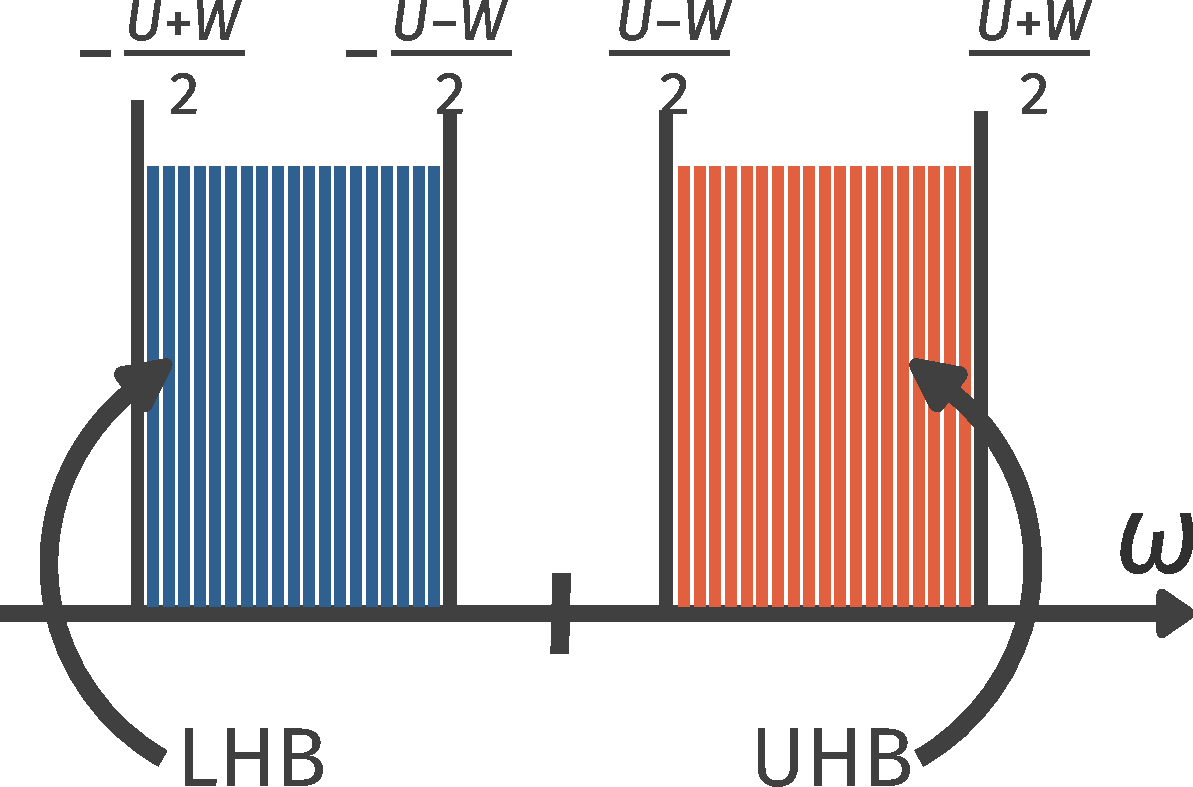
\includegraphics[width=0.48\textwidth]{insulator.pdf}
	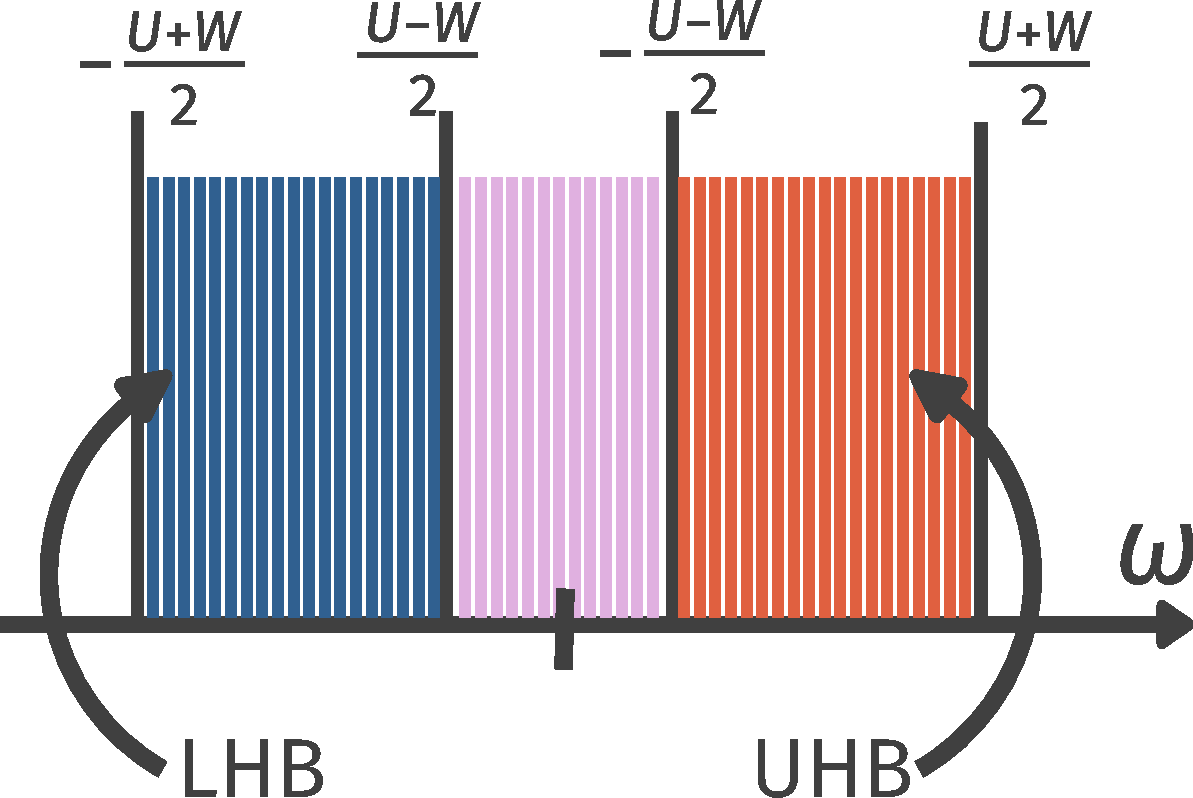
\includegraphics[width=0.48\textwidth]{metal.pdf}
	\caption{}
	\label{HKM-phases}
\end{figure}
The Baskaran-Hatsugai-Kohmoto model~\cite{Baskaran1991,Hatsugai1992} introduced independently in 1991 and 1992 is an exactly solvable model of electronic correlation that displays a transition from a metallic phase to a Mott insulator. While it's solvability offers an instructive method for studying Mott transition, the infinitely long-ranged nature of its interaction makes it tricky to apply these conclusions to realistic materials.

At half-filling, the model is defined by the following Hamiltonian:
\begin{equation}\begin{aligned}
	H_\text{BHK}= \sum_{\bf k,\sigma}\epsilon({\bf k}) n_{\bf k,\sigma} - \frac{U}{2}\sum_{\bf k}(n_{\bf k, \uparrow} - n_{\bf k,\downarrow})^2~.
\end{aligned}\end{equation}
Clearly the model is diagonal in momentum-space; the Hamiltonian splits up into commuting \(4\times 4\) blocks for every point \(\bf k\):
\begin{equation}\begin{aligned}
	H_\text{BHK} = \sum_{\bf k}H({\bf k}), \quad H({\bf k}) = \epsilon({\bf k}) \sum_\sigma n_{\bf k,\sigma} - \frac{U}{2}(n_{\bf k, \uparrow} - n_{\bf k,\downarrow})^2~.
\end{aligned}\end{equation}
The vacant eigenstate \(\ket{0}\) of \(H({\bf k})\) has zero energy (\(E_0 = 0\)), the two singly-occupied states \(\ket{\uparrow}\) and \(\ket{\downarrow}\) have energy \(E_1 = \epsilon({\bf k}) - U/2\) and the doubly-occupied state \(\ket{\uparrow, \downarrow}\) has energy \(E_2 = 2\epsilon({\bf k})\). This leads to two possible single-particle excitations -- one for adding an electron on the vacant state: (\(\Delta_1 = E_1 - E_0 = \epsilon({\bf k}) - U/2\), the other for adding an additional electron on a singly-occupied state: \(\Delta_2 = E_2 - E_1 = \epsilon({\bf k}) + U/2\). 

Upon combining states from other \(k-\)modes, these isolated excitations broaden into bands around \(\pm U/2\) because of the continuum of values available to \(\epsilon({\bf k})\). For large enough \(U\) (compared to the non-interacting bandwidth \(W\)), these bands remain well-separated in energy (Fig.~\ref{HKM-phases} left), forming lower and upper Hubbard bands. The half-filled system results in the lower band being completely filled and the upper band empty, leading to a Mott insulator. The states within this band are all singly-occupied (per \(k-\)state). Upon lowering the correlation strength \(U\), the bands touch each other at the critical value of \(U_c = W\) (obtained by equating the top of the lower band to the bottom of the upper band). For lower values of \(U\), the system is a metal due to the presence of gapless excitations within the combined band (Fig.~\ref{HKM-phases} right). This therefore provides a simple demonstration of a correlation-driven Mott metal-insulator transition.

\section{Strong local correlations and auxiliary models}
\subsection{Introduction to the auxiliary model approach}
One of the main results obtained within this thesis is the development of a formalism to study the more realistic case of finite-dimensional interacting models by using appropriately chosen impurity models as auxiliary models. The key to an {\it auxiliary model method} is to construct an appropriate auxiliary model that while being tractable captures some essential property of the full lattice model~\cite{martin_2016}. This involves separating the complete degrees of freedom into a system part (\(H_S\)) which one treats exactly and the rest of the system (\(H_R\)) that one might simplify in order to be able to solve the problem. The non-trivial nature of the problem arises of course from the hybridisation \(H_{SR}\) between the system and the bath:
\begin{equation}\begin{aligned}
	{H} &= \begin{bmatrix} & {H}_{R} && {H}_{RS} & \\ & {H}_{RS}^* && {H}_{S} & \end{bmatrix}~.
\end{aligned}\end{equation}

This separation can always be done exactly, if one does not care about tractability. For example, one can take the Hubbard model that describes electrons hopping on a lattice and interacting when two electrons reside on the same lattice site:
\begin{equation}\begin{aligned}
	H_\text{hub} = -t\sum_{\langle i,j \rangle,\sigma }(c^\dagger_{i,\sigma}c_{j,\sigma} + \text{h.c.}) + U\sum_{i}n_{i \uparrow}n_{i \downarrow}~,
\end{aligned}\end{equation}
and separate this into parts, the system being the local orbitals of a specific site \(l\) and the rest of the system being all the other sites:
\begin{equation}\begin{aligned}
	H_S = U n_{l \uparrow} n_{l \downarrow},~~ H_R = -t\sum_{\langle i,j \rangle,\sigma }^\prime(c^\dagger_{i,\sigma}c_{j,\sigma} + \text{h.c.}) + U\sum_{i}^\prime n_{i \uparrow}n_{i \downarrow},~~ H_{SR} + H_{RS} = -t\sum_{i,\sigma} (c^\dagger_{l,\sigma}c_{i,\sigma} + \text{h.c.})~,
\end{aligned}\end{equation}
where the primed summation is carried out over all nearest-neighbour pairs that do not involve \(l\) and the summation in \(H_{SR} + H_{RS}\) is over all sites adjacent to \(l\).

The smaller system \(H_S\) (often called the {\it cluster}) is typically chosen such that its eigenstates are known exactly. Progress is then made by choosing a simpler form for \(H_R\) and its coupling \(H_{RS}\) with the smaller system. This combination of the cluster and the simpler bath is then called the \textit{auxiliary system}.
A tractable auxiliary system for the Hubbard model is the single-impurity Anderson model (SIAM); the correlated impurity site represents the set of local orbitals of any given site, while the conduction bath represents the rest of the lattice sites in an approximate fashion.  Such a construction is shown in fig.~\ref{cluster-bath}.
\begin{figure}[!htb]
	\centering
    
\includegraphics[width=0.9\textwidth]{clusterBath.pdf}
	\caption{\textit{Left}: Full Hubbard model lattice with onsite repulsion $U^H$ on all sites and hopping between nearest neighbour sites with strength $t^H$. \textit{Right}: Extraction of the auxiliary (cluster+bath) system from the full lattice. The central site on left becomes the impurity site (red) on the right (with an onsite repulsion $\epsilon_d$), while the rest of the $N-1$ sites on the left form a conduction bath (green circles) (with dispersion $\epsilon_k$ and correlation modelled by the self-energy $\Sigma_k(\omega)$) that hybridizes with the impurity through the coupling $V$.}
	\label{cluster-bath}
\end{figure}

It should be noted that any reasonable choice of the cluster and bath would break the translational symmetry of the full model: To allow computing quantities, one would need to make the bath (which is a much larger system) simpler than the cluster (which is a single site). This distinction breaks the translational symmetry of the Hubbard model. As a result, calculations that make use of the translation symmetry of the full model (such as \(k-\)space objects) will require a periodisation operation of an auxiliary model quantity.
\subsection{Correspondence between impurity and lattice models in $d=\infty$}

Dynamical Mean-Field Theory (DMFT) provides a nonperturbative framework for treating strong local electronic correlations in lattice models by mapping them onto a self-consistent quantum impurity problem \cite{Metzner1989,Georges1996}. The central idea of DMFT is that in the limit of infinite spatial dimension, or equivalently infinite coordination number, the electronic self-energy becomes purely local while retaining its full dynamical (frequency-dependent) structure. As a result, the many-body lattice problem reduces to an effective single-site problem embedded in a self-consistently determined bath, capturing local quantum fluctuations exactly while neglecting nonlocal correlations. DMFT has become a cornerstone of modern correlated-electron theory, successfully describing Mott metal--insulator transitions, quasiparticle formation, and spectral weight transfer in Hubbard-like models \cite{Georges1996,Kotliar2004,Georges2004}.

In order to motivate the impurity model-lattice model mapping inherited by DMFT, we first recall the textbook example of classical mean-field theory. Mean-field theory provides one of the earliest and most instructive examples of controlled approximations in many-body physics. In its classical incarnation, exemplified by the Ising model,
\begin{equation}
	H_{\mathrm{Ising}} = - \sum_{i\neq j} J_{ij} S_i S_j - h \sum_i S_i = -\sum_i S_i(h + \sum_{j \neq i}J_{ij}S_j),
\end{equation}
mean-field theory proceeds by replacing the interaction between a given spin and its neighbors by an {\it effective static field} proportional to the average magnetization. Writing
\(
S_j = \langle S_j \rangle + \delta S_j
\)
and neglecting quadratic fluctuations and constant parts, one obtains an {\it auxiliary problem} in the form of a mean-field Hamiltonian
\begin{equation}\begin{aligned}
	H^{(\text{MF})}_{\mathrm{Ising}} = - \sum_{i} (h + h_\text{MF}(i))S_i~,
\end{aligned}\end{equation}
where the mean-field \(h_\text{MF}\) comes out to be
\begin{equation}\begin{aligned}\label{mean-field}
	h_\text{MF}(i) = \sum_{j \neq i}2 \langle S_j \rangle J_{ij}~.
\end{aligned}\end{equation}
The above approach assumes two things: (i) the presence of a non-zero {\it order parameter} \(m_j = \langle S_j \rangle \) (in this case, a non-zero magnetisation), and (ii) the smallness of the fluctuations \(S_j - \langle S_j \rangle\). The mean-field Hamiltonian can be used to compute the partition function (at inverse temperature \(\beta\)) and hence the magnetisation at a site \(i\) of the lattice:
\begin{equation}\begin{aligned}\label{magnetisation}
	m_i = \tanh(\beta(h_\text{MF}(i) + h)) = \tanh(\beta \sum_{j \neq i}2 m_j J_{ij} + \beta h)~.
\end{aligned}\end{equation}

The problem hasn't yet been solved of course; one needs to determine the appropriate value of \(m_j\). We therefore need an additional equation; this is provided by the so-called {\it self-consistency condition}. The translation invariance of the lattice ensures that the magnetisation must be uniform across sites \(i\) and \(j\). This allows us to replace \(m_j\) with \(m_i\) in the above equation:
\begin{equation}
	m_i = \tanh(\beta m_i\sum_{j \neq i}2 J_{ij} + \beta h)~.
\end{equation}
This equation can be solved numerically to obtain the uniform magnetisation \(m_i = m\).
The mean-field approximation becomes exact in the limit of large coordination, where fluctuations are suppressed  and spatial correlations beyond a single site vanish.

An equivalent way of framing the self-consistency equation is to equate the mean-fields on different lattice sites. Combining eqs.~\ref{magnetisation} and \ref{mean-field}, we have
\begin{equation}\begin{aligned}
	h_\text{MF}(i) = \sum_{j \neq i}2 m_j J_{ij} = \sum_{j \neq i}2 \tanh(\beta(h_\text{MF}(j) + h)) J_{ij}~.
\end{aligned}\end{equation}
The equation in terms of \(h_\text{MF}(i)\) and \(h_\text{MF}(j)\) can again be solved numerically by claiming that the mean-field has to be uniform across all the sites owing to translation invariance. This form of the self-consistency requirement (in terms of the field) will be useful to us in the upcoming discussion.


The essential feature of classical mean-field theory is therefore the replacement of a many-body problem by an effective \emph{single-site} problem embedded in a self-consistently determined environment. Quantum lattice models admit a closely analogous construction, but with an important conceptual difference: while the classical mean field is static, quantum fluctuations necessarily introduce a tower of excited states that allow for temporal dynamics. This observation underlies the formulation of dynamical mean-field theory (DMFT), which may be viewed as the natural quantum generalization of classical mean-field theory \cite{metzner_volhardt_1989,georges1996}.

Similar to the previous case of the Ising model, we will now derive the self-consistency equation for a quantum model. Consider an interacting fermionic lattice Hamiltonian, such as the Hubbard model:
\begin{equation}
H = -\sum_{ij\sigma} t_{ij} c_{i\sigma}^\dagger c_{j\sigma}
+ U \sum_i n_{i\uparrow} n_{i\downarrow},
\end{equation}
defined on a lattice with coordination number \(z\). 
% To obtain a nontrivial limit as \(z \to \infty\), the hopping amplitudes are scaled as
% \begin{equation}
% t_{ij} = \frac{t^\ast}{\sqrt{z}},
% \end{equation}
% which ensures a finite kinetic energy per site \cite{MetznerVollhardt1989}.

% In this limit, it can be shown diagrammatically that all nonlocal contributions to the self-energy vanish as inverse powers of \(z\), while local diagrams remain finite. As a result, the exact self-energy becomes purely local,
% \begin{equation}
% \Sigma_{ij}(\omega) = \delta_{ij}\,\Sigma(\omega),
% \end{equation}
% though it retains its full dynamical (frequency-dependent) character \cite{MetznerVollhardt1989,Georges1996}.

The point of this exercise is to calculate the interacting self-energy \(\Sigma_k(\omega)\) for the fermions. This therefore acts as an ``order parameter" and plays the same role as the local magnetisation in the previous exercise. The self-energy defines the interacting \(k\)-space Green's function for a translation-invariant problem:
\begin{equation}
	G_{\mathbf{k}}(\omega) = \frac{1}{\omega - \varepsilon_{\mathbf{k}} - \Sigma_{\mathbf{k}}(\omega)},
\end{equation}
where \(\varepsilon_{\mathbf{k}}\) denotes the noninteracting dispersion, and a real-space local Green's function, obtained by summing over momentum:
\begin{equation}\label{eq:localG}
G_{\text{loc}}(\omega) = \sum_{\mathbf{k}} \frac{1}{\omega - \varepsilon_{\mathbf{k}} - \Sigma_{\mathbf{k}}(\omega)}.
\end{equation}

Similar to the earlier exercise, we need to apply a mean-field decoupling to drop certain fluctuations and obtain a similar effective problem. In the context of interacting electrons, such a decoupling is obtained in the limit of infinite dimensionality or coordination number, where the self-energy becomes \(k-\)independent~\cite{metzner_volhardt_1989}:
\begin{equation}\begin{aligned}
	\Sigma_{\mathbf{k}}(\omega) = \Sigma_\text{loc}(\omega), \text{ or (equivalently) }~ \Sigma_{ij}(\omega) = \delta_{ij}\Sigma_\text{loc}(\omega)~.
\end{aligned}\end{equation}
The mean-field decoupling here therefore corresponds to ignoring spatial fluctuations of the one-particle self-energy, and leads to a local Greens function that is directly connected to the local self-energy:
\begin{equation}\begin{aligned}
G_{\text{loc}}(\omega) = \sum_{\mathbf{k}} \frac{1}{\omega - \varepsilon_{\mathbf{k}} - \Sigma_\text{loc}(\omega)}.
\end{aligned}\end{equation}
It turns out that a local Greens function connected to a local self-energy also defines a quantum impurity problem describing the dynamics of a single correlated site with the other environment sites integrated out:
\begin{equation}\label{effAction}
	S_{\text{imp}} = -\int_0^\beta d\tau d\tau'\,c^\dagger(\tau)\,G_\text{MF}^{-1}(\tau-\tau')\,c(\tau') + U \int_0^\beta d\tau\, n_\uparrow(\tau) n_\downarrow(\tau).
\end{equation}
This acts as an auxiliary problem for the more complete problem locally interacting electrons on a lattice. The non-interacting Greens function \(G_\text{MF}\) is as of now unknown, and defines the environment of the impurity site and comprises the dynamics of the sites that have been integrated out. Such an impurity problem is solvable, and the impurity Green's function is given by
\begin{equation}
	G_{\text{imp}}(\omega) = \frac{1}{G_\text{MF}^{-1}(\omega) - \Sigma_\text{imp}(\omega)},
\end{equation}

The first term in eq.~\ref{effAction} is therefore what makes this problem dynamical -- it represents the probability of electrons hopping into and out of the impurity site, and leads to fluctuations of its occupancy. We can make the identification of the Greens function \(G_\text{MF}\) as the {\it mean-field} encountered in the previous example. More specifically, \(G_\text{MF}\) acts as a ``field" because it is obtained by integrating out the other sites on the lattice, and it acts on the impurity site by affecting its dynamics.

The complete set of equations for the solving such a dynamical mean-field problem is finally obtained by equating the impurity local Greens function \(G_\text{imp}\) to the lattice local Greens function \(G_\text{loc}\). As discussed earlier, such a solution exists in an exact fashion only in the limit of infinite dimensions, as long as the correct \(G_\text{MF}\) can be found. In order to find the appropriate \(G_\text{MF}\) that allows equating the impurity model Greens function to a lattice mode Greens function, we require an additional equation: the self-consistency condition. Similar to the case of the Ising model, we require that \(G_\text{MF}\) be equal to \(G_\text{loc}\), owing to translation invariance. The full set of coupled DMFT equations is
\begin{equation}\begin{aligned}
	G_\text{MF}	&= G_\text{loc},\\
	\Sigma_\text{imp}(\omega) &= G_\text{MF}^{-1}(\omega) - G^{-1}_{\text{imp}}(\omega),\\
	\Sigma_\text{loc}(\omega) &= \Sigma_\text{imp}(\omega),\\
	G_{\text{loc}}(\omega) &= \sum_{\mathbf{k}} \frac{1}{\omega - \varepsilon_{\mathbf{k}} - \Sigma_\text{loc}(\omega)}.
\end{aligned}\end{equation}
\begin{itemize}
	\item The first equation is equivalent to the feature in the previous exercise where we equated the mean-fields on \(i\) and \(j\).
	\item The second equation is equivalent to computing, in the previous exercise, the magnetisation on the \(j^\text{th}\) site from the partition function.
	\item The third equation is the essential mean-field approximation, where we equate the self-energy of the simpler decoupled problem to that of the more complete lattice problem and is justified in the limit of infinite dimensions.
	\item The fourth equation is equivalent, in the previous exercise, to using the computed ``magnetisation" of site \(j\) in the second step to further compute the mean-field at site \(i\).
\end{itemize}

In direct analogy with classical mean-field theory, DMFT replaces a lattice model by an effective single-site problem embedded in a self-consistent environment. The crucial distinction is that the mean field is now dynamical rather than static, encoding quantum fluctuations exactly while neglecting spatial correlations. Importantly, this demonstrates the importance of quantum impurity models in investigating correlated lattice models, particularly in the presence of strong local interactions. This is because the effects of local correlations are captured exactly by such an auxiliary model mapping.

\subsection{Examples of strongly correlated materials}
As discussed in the previous section, the route to studying lattice problems via quantum impurity models makes most sense for models with strong local correlations. 

\paragraph{Transition Metal Oxides (TMOs)}
Transition Metal Oxides (TMOs) are defined chemically by the presence of partially filled $d$-shells in transition metals (e.g., Cu$^{2+}$, Mn$^{3+}$, V$^{4+}$) coordinated by oxygen ligands. The physics of TMOs is governed by the competition between the kinetic energy hopping amplitude $t$ and the on-site Coulomb repulsion $U$; due to the small overlap between the localised \(d-\)orbitals, the \(d-\)electrons can delocalise only by hopping onto the ligand atoms. According to the Zaanen-Sawatzky-Allen (ZSA) classification scheme~\cite{Zaanen1985}, these materials are categorized as either Mott-Hubbard insulators, where the charge gap is determined by the $d$-$d$ Coulomb interaction ($E_g \approx U$), or charge-transfer insulators, where the gap is dictated by the energy difference between the oxygen $p$-band and the metal $d$-band. These derive from considerations of several factors, such as crystal field splitting, arrangement of atoms and lattice symmetries. 

For example, in the case of octahedral symmetry, repulsion from the surrounding atoms leads to the raising of energy of the \(d_{x^2 - y^2}\) and \(d_{3z^2-r^2}\) orbitals forming the \(e_g\) doublet, while the other three orbitals (\(d_{xy}, d_{yz}\) and \(d_{zx}\)) form the \(t_{2g}\) multiplet. For the heavier TMOs (Ti, V, Cr...), the Fermi level lies within \(e_{g}\). The increased positive nuclear charge (compared to the lighter elements) lowers the energy of the \(d-\)orbitals and brings them closer to the \(p-\)orbitals, reducing the charge transfer energy \(\Delta = \varepsilon_d - \varepsilon_p\) of transporting an electron from a \(d-\)state to a \(p-\)state, compared to the \(d-\)level repulsion \(U\) (\(|\Delta| < U\)). Geometric reasons (the \(e_g\) orbitals point towards the \(p-\)orbitals) also enhance the hybridisation between \(d-\) and \(p-\)orbitals in such materials. If \(\Delta\) becomes larger than the bandwidth, we obtain a {\it charge-transfer insulator}, where the charge gap is decided by \(\Delta\). In the lighter TMOs, the Fermi level passes through \(t_{2g}\), and because they point away from the \(p-\)orbitals, the hybridisation is weaker. Moreover, the reduced positive nuclear charge leads to an increased \(\Delta > U\); a \(U\) greater than the bandwidth leads to what's called a {\it Mott-Hubbard insulator}.

Experimental studies of transition metal oxides (TMOs) have established metal–insulator transitions (MITs) as a defining consequence of strong electronic correlations in systems with partially filled (d)-electron shells \cite{Imada1998,mcwhan1969}. Early experiments on vanadates such as $V_2O_3$ characterised pressure-driven MITs through the pressure- and temperature-dependent conductivity as well as an anomalous enhancement of the optical conductivity\cite{Limelette2003,Rozenberg1995,Qazilbash2007}. Copper oxides constitute the most extensively studied class of correlated TMOs and provide a canonical example of a doping-driven MIT. Transport measurements on parent compounds such as $La_2CuO_4$ establish a robust insulating state, while carrier doping leads to anomalous metallic behavior characterized by linear-in-temperature resistivity and unconventional superconductivity\cite{Takagi1992,Ando2004,Lemberger2011}. Such metal-insulator transition is also reported from angle-resolved photoemission spectroscopy (ARPES) measurements in doped $La_2CuO_4$ and $Bi_2Sr_2CaCu_2O_8$, along with the emergence of pseudogap near the antinodes at high temperatures and a hole-to-electronlike Fermi surface reconstruction\cite{Damascelli2003,Sobota2021,Vishik_2018}. Nickelates ($LaNiO_2$, $La_3Ni_2O_7$, $La_4Ni_3O_{10}$, etc) exhibit related but distinct experimental signatures. With \(Ni^+\) sharing the same \(3d^9\) valence configuration as \(Cu^{2+}\) in the cuprate superconductors, these materials also display superconductivity, although the mechanism in the nicklelates is different due to the strong coupling between the layers~\cite{Medarde_1997,Wang2025}. The optimal doped regime in thin films shows strange metal behaviour, while infinite-layer nickelates show the absence of long-range antiferromagnetic order~\cite{Puphal2026}.

\paragraph{Transition Metal Dichalcogenides}
Transition Metal Dichalcogenides (TMDs) are layered van der Waals materials with the stoichiometry $MX_2$, where $M$ is a transition metal (e.g., Mo, W) and $X$ is a chalcogen (e.g. S, Se, Te)~\cite{Manzeli2017,Joseph2023}. Recent interest has focused on the interplay between strong spin-orbit coupling (SOC), electronic correlations and direct bandgap -- properties that make them particularly useful for electronic applications, spintronics and DNA sequencing. Layered TMDs have the structure \(X-M-X\), with the transition metal sandwiched between two hexagonal planes of chalcogenides. Different combinations of the metals with the chalcogens lead to widely varying structures and electronic properties in TMDs. Experimental studies show that metal--insulator transitions (MITs) in TMDs are commonly intertwined with charge density wave (CDW) formation rather than arising from purely on-site Coulomb localization~\cite{Wilson1974PRL,Wilson2001}. In prototypical compounds such as 1T-TaS$_2$, ARPES and transport measurements reveal fluctuating magnetic order parameters in the Mott state and a transition to superconductivity driven by pressure \cite{Fazekas1979,Perfetti2005,Sipos2008}. Scanning tunnelling microscope (STM) pulses have been successfully used to manipulate the metal–insulator transition of 1T-TaS2, demonstrating the macroscopic controllability of the Mott phase\cite{Cho2016}.

ARPES measurements in 2H-NbSe$_2$ and 2H-TaSe$_2$ partial gapping of the Fermi surface restricted to nested momentum regions and a temperature-dependent pseudogap similar to the cuprates\cite{Borisenko2008,Borisenko2009}. This is further supported by optical conductivity experiments that show spectral weight in the midinfrared region along with a low-frequency Drude contribution~\cite{Vescoli1998}. Transport measurements on single crystals of TaSe$_2$ reveal that disorder enhances superconductivity by suppressing other competing orders such as CDW~\cite{Li2017}. Collectively, these experimental results establish TMDs as a distinct class of correlated materials in which reduced dimensionality, band narrowing, and lattice reconstruction cooperate to produce metal--insulator behavior beyond conventional band theory.

\paragraph{Iron-Based Superconductors}
The iron-based superconductors (FeSCs), discovered in 2008, constitute a broad family of layered materials that share a common structure: a layer of iron atoms joined by tetrahedrally coordinated pnictogen (P, As) or chalcogen (S, Se, Te) anions arranged in a stacked sequence; the layers are separated by alkali, alkaline-earth or rare-earth and oxygen/fluorine ‘blocking layers’\cite{kamihara2008,Paglione2010,Hirschfeld2011,stewart2011}. Doping or applying external pressure reveals coupled antiferromagnetic and structural transitions along with superconducting and nematic orders~\cite{Johnston2010,Kasahara2012,Fernandes2014}. Electrical resistivity measurements in the neighbourhood of the quantum critical point show a crossover from a bad-metal behavior (\(T-\)linear resistivity)  to a Fermi liquid behaviour (\(T^2-\)resistivity) \cite{Analytis2014}. Optical conductivity measurements indicate point to intermediate-to-strong electronic correlations \cite{Qazilbash2009}.

ARPES measurements reveal a \(k-\)dependent superconducting gap and de Haas-van Alphen measurements indicate substantial quasiparticle mass enhancements, shedding more light on the correlated nature of the material\cite{Shishido2010,terashima2009}. Strain-tuning measurements of the nematic susceptibility, and differential elastoresistance measurements have provided compelling evidence for the nematic transition and its surrounding fluctuations being the cause of the structural transition as well as the superconductivity\cite{Chu2012,Kuo2016}. Neutron scattering and NMR measurements further reveal persistent low-energy spin fluctuations across wide regions of the phase diagram, supporting scenarios in which unconventional superconductivity emerges from the interplay of magnetic, orbital, and nematic degrees of freedom \cite{Inosov2010,Chubukov2012}.

\paragraph{Heavy-Fermion / Kondo-Lattice Systems}
Heavy-fermion materials are a class of strongly correlated electron systems typically realized in intermetallic compounds of rare earth metals (such as Ce, Sm and Yb) and actinides (such as U, Np and Pu), where localized $f$ electrons hybridize with itinerant conduction bands \cite{Stewart1984,Wirth2016}. At high temperatures, these systems exhibit local-moment behavior governed by Curie--Weiss susceptibilities and incoherent transport, while at low temperatures the Kondo effect leads to the formation of a coherent many-body state with extremely large quasiparticle effective masses \cite{hewson1993}. Experimentally, this crossover is most clearly manifested in transport and thermodynamic measurements: the electrical resistivity shows a characteristic maximum followed by a rapid drop signaling the onset of coherence, while the linear specific heat coefficient $\gamma=C/T$ reaches values orders of magnitude larger than in conventional metals, directly reflecting the heavy quasiparticle mass \cite{Lohneysen2007}.

A defining feature of heavy-fermion materials is their proximity to magnetic quantum phase transitions, which can be accessed experimentally by pressure, chemical substitution, or magnetic field~\cite{Gegenwart2008}. Near such quantum critical points (QCPs), transport measurements reveal pronounced non-Fermi-liquid behavior ($T-$linear resistivity) and a vanishing Hall response, along with a divergent effective quasiparticle mass as the transition is approached~\cite{Custers2003,Paschen2004}; these are all indications of the breakdown of electronic excitations near the transition. Neutron scattering experiments provide direct evidence for spin fluctuations down to very low temperatures, interplaying with the itinerant electrons at the QCP and potentially driving the superconducting transition~\cite{Schroder2000,Stockert2011}. Quantum oscillation measurements through de Haas–van Alphen experiments further demonstrate Fermi surface reconstruction across the quantum critical point, highlighting the drastic change in Fermi volume~\cite{Shishido2005}. Together, these experimental observations establish heavy-fermion compounds as paradigmatic systems in which strong local correlations, hybridization-driven coherence, and quantum critical fluctuations conspire to produce emergent low-energy quasiparticles and unconventional metallic behavior~\cite{Si2010}.

\section{Phenomenology of the Anderson impurity model}
Within this thesis, we have developed an auxiliary model approach that combines the physics of quantum impurity models with a manybody version of Bloch's theorem to investigate interacting fermionic lattice models. This is motivated by the relative ease in solving impurity models and transparency afforded by such solutions. We now review the phenomenology of some of these impurity models and point out how the various impurity features affect the physics of the lattice models.

The single-impurity Anderson model describes the dynamics of a system of non-interacting itinerant electrons \((c_{k,\sigma})\) hybridising with a localised correlated impurity orbital (\(d_\sigma\))~\cite{Anderson1959}:
\begin{equation}\begin{aligned}
	H_\text{AIM} = \sum_{k,\sigma}\epsilon_k n_{k,\sigma} + \sum_{k,\sigma}V_k(c^\dagger_{k,\sigma}d_\sigma + \text{h.c.}) + \epsilon_d \sum_\sigma n_{d\sigma} + Un_{d \uparrow} n_{d \downarrow}~.
\end{aligned}\end{equation}
\(V_k\) controls the hybridisation strength, and \(\epsilon_d\) and \(U\) control the onsite energy and local correlation respectively of the impurity site. In the limit of large \(U\), the impurity dynamics gets projected onto its spin states, and the model then describes the scattering of non-interacting electrons off magnetic impurities, through the Kondo model:
\begin{equation}\begin{aligned}
	H_\text{Kondo} = \sum_{k,\sigma}\epsilon_k n_{k,\sigma} + J \sum_{k_1,k_2}\sum_{\alpha,\beta}\vec{S}_d \cdot \vec{\sigma}_{\alpha,\beta}c^\dagger_{k_1,\alpha}c_{k_2,\beta}~,
\end{aligned}\end{equation}
where \(\vec{S}_d\) is the impurity spin formed by projecting the Hilbert space of the impurity to the singly-occupied states.

Even though the conduction bath is non-interacting, the presence of local repulsion on the impurity site makes the problem {\it many-electron} in nature: it makes it impossible to study the electrons in isolation. This can be seen as follows: imagine two conduction electrons \(\ket{k_1 \uparrow}\) and \(\ket{k_2 \downarrow}\) trying to hybridise with an empty impurity site. The first electron moves onto the impurity site through a scattering process of the form \(c^\dagger_{d \uparrow}c_{k_1 \uparrow}\) and makes the impurity site single occupied (\(\ket{\uparrow}_d\)), but now the second electron \(k_2\) {\it must pay a cost} of the order of \(U\) in order to hybridise with this singly-occupied impurity site through a process of the kind \(c^\dagger_{d \downarrow}c_{k_1 \downarrow}\). This shows that the conduction electrons {\it are aware} of the other electrons, and all of them must be treated together. Another way of seeing this collective behaviour is from the Kondo model. Again imagine two two spin-up electrons \(k_1,k_2\) that are about to scatter off the impurity spin (which is presently down) via a {\it spin-flip} process. The first electron scatters and leaves the impurity spin up while it itself becomes down, but now the second conduction electron cannot spin-flip scatter because the spins cannot be exchanged (both are down!). This is another example of how the conduction electrons can {\it feel} the presence of the other electrons, and this is what makes the problem many-electron in nature.

Despite the interacting nature of the problem, the problem can be solved in an effectively exact fashion, via Wilson's numerical renormalisation group approach~\cite{wilson1975renormalization}, or the method of {\it Bethe ansatz}~\cite{andrei_1980,Wiegmann_1981}. The former solution is more transparent: for any non-zero value of the hybridisation \(V\) (or Kondo coupling \(J\)), the low energy physics of the impurity is described by a strong-coupling fixed point, where the impurity forms a maximally-entangled singlet state with the local spin density of the conduction bath. The low-energy excitations about such a fixed point can be calculated from renormalised perturbation theory, and describe a local Fermi liquid -- one particle excitations in the neighbourhood of the singlet renormalised by a local repulsion term~\cite{nozieres1974fermi}. The crossover from the free local moment at high temperatures to the screened non-magnetic state at low temperatures occurs at an emergent energy scale \(T_K\), the Kondo temperature, which depends exponentially on the strength of the Kondo coupling, and is the only energy scale remaining at low temperatures, so that all thermodynamic quantities must go as a function of \(T/T_K\)~\cite{wilson1975renormalization}.

\subsection{DMFT results on the Bethe lattice}
, and has been studied using an equally diverse array of methods like mean-field theory, renormalisation group approaches, numerical techniques like exact diagonalisation, quantum Monte Carlo and dynamical mean-field theory, and many others. In particular, dynamical mean-field theory (DMFT)~\cite{kuramoto1987,Cox1988,metzner_volhardt_1989,zhang_1993,georges1996,parcollet_2004,maier_2005,kotliar_2006,ohashi_2008} obtains an exact solution of the Mott metal-insulator transition (MIT) for the 1/2-filled Hubbard model~\cite{Mott_1949,gutzwiller_1963,kanamori_1963,hubbard1963electron,brinkman_rice_1970} on the Bethe lattice with infinite coordination number, in terms of an Anderson impurity model with a self-consistently determined bath obtained by requiring, in an iterative manner, that its local Greens function be equal to that of the impurity site. The above-mentioned transition can be captured by the local spectral function through (i) the continuous appearance of a Mott gap, followed by (ii) the sharpening and vanishing of the central Kondo resonance. These two features are often referred to, respectively, as the Mott-Hubbard~\cite{hubbard1963electron} and Brinkman-Rice~\cite{brinkman_rice_1970} scenarios of the Mott MIT. The exact nature of the solution arises from the fact that all non-local contributions to the lattice self-energy are observed to vanish upon taking the limit of an infinite coordination number for the lattice model.
\subsection{Open Questions}

\section{Effect of low dimensionality: Mott MIT in two dimensions}
\subsection{DCA, CDMFT results (among other methods)}
\subsection{Experimental results}
\subsection{Open Questions}

\section{Effect of multiple bands: Orbital selective Mott transition}
\subsection{results on heavy fermions}
\subsection{Experimental results}
\subsection{Open Questions}

\section{Brief introduction to the tiling auxiliary model approach}
\subsection{Why do we need another auxiliary model method? Limitations of existing approaches}
\subsection{Overview}
\subsection{Features}

\section{Entanglement, RG, and Fermionic Criticality}
\subsection{Introduction to entanglement holography}
\subsection{Open questions}

\section{<title about an introduction to our holography work>}

The present millennium has seen a rapid surge in the use of quantum entanglement towards the study of quantum and condensed matter systems~\cite{terhal_physicstoday_2003,horodecki2009quantum,eisert_entanglement_2010,laflorencie2016quantum,zeng2019,Erhard2020}. By tracking quantum correlations among particles across both small and large distances, entanglement measures offer valuable insights into the nature of the ground state and low-energy excitations. This, for example, allows us to distinguish strongly-correlated topologically ordered states characterised by long-ranged entanglement (in the form of a sub-leading topological term in their entanglement entropy~\cite{wen_1990,Wen_fqhe_1990,wen1995topological,niu1985quantized}) from weakly-interacting topologically trivial phases that have short-ranged area-law entanglement~\cite{das_shankaranarayanan_2006,cramer_eisert_2006,eisert_entanglement_2010}.

More pertinent to the present work is the entanglement of non-interacting relativistic fermionic systems. Such phases are known to emerge in several condensed matter systems~\cite{vafek_2014_diracreview}, appearing at the surfaces of three-dimensional topological insulators~\cite{bernevig_2013,cayssol2013,moessner_moore_2021,Rachel_2018}, quasi-2D organic materials~\cite{wang_2015,Wu_2016,ni_2022_dirac} and in artificial quantum simulators such as cold atom gases, molecular and microwave crystals~\cite{zhu_2007_coldatoms,Lepori_2010,Boada_2011,Kuno2018,Gomes2012,Yuan2016,bellec_2013}.
Massless critical systems (or conformal field theories (CFTs)) differ from gapped systems due to the fact that their entanglement satisfies a modified area law; in one spatial dimension, the entanglement entropy ($S$) of a single subsystem of length \(l\) scales as \(S \sim \frac{c}{3}\ln l\)~\cite{vidal2003entanglement,latorre_extanglement_2003,lattore_pra_2005,calabrese2004,wolf2008area}, where \(c\) is the conformal central charge of the CFT.
This violation arises from the non-local nature of the gapless quantum fluctuations that lie proximate to the $d-1$-dimensional Fermi surface of a quantum critical fermionic system in $d$ spatial dimensions.
For massive fermions, an entropic \(c-\)function (spatial derivative of the entanglement entropy) can be expressed in the form of differential equations that need to be solved numerically~\cite{Casini_2005,Cardy2008,Casini_2009_multi,doyon_2009}.

Unlike topologically ordered phases, there is no geometry-independent topological term in the entanglement entropy of free fermionic systems~\cite{Chen_2017,bueno_2017}. It is, however, possible to generate such a term even here by placing the system on a multiply connected manifold such as a cylinder, and inserting a magnetic flux through the cylinder~\cite{Metlitski_2009,Arias_2015,Whitsitt_2017,Chen_2017,zhu_kagome_2018}.
It has been shown that if there are \(\phi\) number of electronic flux quanta piercing the system, an additional term is generated in the entanglement entropy of a subsystem of massless Dirac fermions of sufficiently large length (as defined in Ref.~\cite{Chen_2017}) with the form $\frac{1}{6}\ln \big|2\sin \frac{\phi}{2}\big|$~\cite{Chen_2017,Arias_2015}. Further, there is evidence from numerical computations on discrete models that such a term is a signature of the specific field theory and encodes universality~\cite{zhu_kagome_2018,Hu_triangular_2019,crepel_2021}.

The notion of entanglement also plays a key role in the context of holographic duality, which posits that there exists a duality relation between a quantum field theory in \(d-\)spatial dimensions and a gravity theory in \(d+1-\)spatial dimensions~\cite{hooft_1974,polyakov_1978,polyakov_strings,gross_1993,bousso_2002,zaanen_liu_sun_schalm_2015,hartnoll_lucas_sachdev2018}. It is widely believed that the additional dimension can be visualised as a renormalisation group flow that starts from the (almost) critical field theory on the boundary and extends into the bulk~\cite{akhmedov_1998,alvarez_1999,freedman_1999,porrati_1999,kachru_2000,girardello_2000,de2000,
de_2001,Johnson_2001,Yamaguchi_2003}. The most popular realisation of the holographic principle is the AdS/CFT correspondence that links a conformal field theory with a theory of quantum gravity through a strong-weak duality relation~\cite{bekenstein_1973,Hawking_1974,Hawking_1975,maldacena1999large,gubser_1998,witten1998anti,
ryu2006,ryu2006aspects}.
This has led to new insights in various areas of high energy and condensed matter physics, such as the viscosity of the quark-gluon plasma~\cite{kovtun_2005}, the response functions of the Bose-Hubbard model~\cite{damle_1997,hartnoll_2007}, and the phenomenology of non-Fermi liquids~\cite{lee_2009_nonfermi,lio_2011,faulkner_2011,mihailo_2009}, holographic superconductors~\cite{gubser_2010,gauntlett_2009,hartnoll_2008_building,Hartnoll_2008,Cai2015,Wang2020}, striped phases~\cite{Donos2011,Donos2013,Cremonini2018} and holographic Fermi liquids~\cite{kachru_2008,cubrovic_2011,senthil_2003,sachdev_2011,Hartnoll_2011_stellar}.

Conversely, the holographic principle also implies that studying the boundary conformal theory can provide insights into the nature of the bulk quantum gravity theory. This requires constructing the emergent dimension from first principles by investigating the RG flow of the (often strongly coupled) quantum field theory, and has proved to be considerably more difficult.
Nevertheless, there exist some examples of constructive attempts towards a bulk gravity theory, including ~\cite{matsueda_2012_kondo,czech_2018,Lee2012,lee2014,vidal2007,vidal2008,swingle2012a,evenbly_2014,anirbanurg1,anirbanurg2}.
These include the momentum-shell renormalisation approach of Refs.\cite{lee2010,lee_2010_lectures,Lee2012,lee2014}, the multi-scale entanglement renormalisation ansatz (MERA) approach of Refs.\cite{vidal2007,vidal2008,swingle2012a,evenbly_2014,milsted_2018}, the exact holographic mapping (EHM)~\cite{qi2013,lee2016}, the Wilsonian RG-based approach of Ki-Seok Kim~\cite{kim2019,kim_2017_supeconductor,kim_2016} and the unitary renormalisation group (URG) approach~\cite{anirbanurg1,anirbanurg2,Mukherjee_mott_merg}.

Questions on entanglement and holography become particularly interesting in systems of critical fermions. As mentioned earlier, such systems differ from bosonic and gapped systems through the presence of longer-ranged entanglement that follows a modified area-law~\cite{wolf2008area,swingle2010} as well as topological features arising from the incompressibility of the Fermi volume~\cite{oshikawa2000topological,seki2017topological}. Fermi surface gapping phase transitions in such systems are often driven by changes in topological quantum numbers and the nature of the inter-particle entanglement~\cite{anirbanurg1,anirbanurg2,Gegenwart2008}. Constructing a framework for fermionic criticality is therefore an active area of research with consequences for important systems such as unconventional superconductors, strange metals and heavy fermions~\cite{anirbanmott1,anirbanmott2,anirban_mott_2022,Custers2003}. Still less is known about the holographic implications of such systems. We extend this body of work by providing an explicit demonstration of the holographic principle in the form of a simple and tractable exact holographic mapping (EHM) for a free fermion system with and without a mass gap. Our program yields analytic relations between the RG flow parameters and their dual bulk quantities such as distances and curvature. This also allows us to study the consequences of a critical Fermi surface (lying precisely at the quantum phase transition) on the nature of the holographic space.

% \include{methods/methods.tex}
\include{ESIAM/esiam.tex}
% \include{tileForm/tileForm.tex}
\chapter{Mott Criticality as the Confinement Transition of a Pseudogap-Mott Metal: Insights from a lattice-embedded impurity model}

\section{Introduction}
The Landau quasiparticle paradigm~\cite{landau1959theory} underpins our understanding of metallic behaviour, where the screening of long-ranged repulsive interactions between delocalised electrons leads to well-defined excitations that carry the same quantum numbers as free electrons. This remarkable phenomenon - known as adiabatic continuity -  is captured by excitations described by poles of the single-particle Greens function of the interacting system. But what defines metallicity when quasiparticles are no longer well-defined~\cite{Phillips2013Unparticles}? Can a surface of zeros of the Greens function~\cite{dzyaloshinskii2003some}, rather than poles forming a Fermi surface, define an entirely new kind of metal? Could such an exotic state serve as the precursor to Mott localisation driven purely by repulsion, and without invoking magnetic order~\cite{Mott_1949}? These questions necessitate a radical departure in understanding conduction in correlated electron systems beyond the quasiparticle paradigm~\cite{phillips2022}. \\

\noindent
The anomalous pseudogap (PG) phase, observed in the cuprates, exhibits nodal-antinodal dichotomy with spectral weight concentrated on Fermi arcs around the nodal regions~\cite{loeserKapitulnik1996, Norman1998, Hashimoto2014}. In the PG phase of such Mott systems
~\cite{taillefer2010,FradkinRevModPhys2015,Sato2017,DoironLeyraud2017,Mukhopadhyay2019,Naman2021,Masafumi2025,KyungKotliar2006,MacridinAzevedo2006,sakai2009evolution,werner2009momentum,sakai2010doped,lin2010,gull2010momentum,gull2012,Mirzaei2013,gull2013,anirbanmott2,HilleAndergassen2020,Jiang2022,Scheurer2018,Krien2022,Kitatani2023,Sorella2023,Schafer2021,White1998,Ido2018,ProustTaillefer2019,Ponsioen2019,XuZhang2022}, the single-particle Green’s function develops surfaces of zeros, also known as Luttinger surfaces~\cite{Phillips2013,dzyaloshinskii2003some}, that signals a fundamental obstruction to quasiparticle formation. As interaction strength increases, these zero surfaces proliferate, fragmenting the Fermi surface into nodal arcs~\cite{sakai2009evolution,Phillips2013}, violating the Luttinger sum rule by reconfiguring Fermi volume~\cite{seki2017topological}, and breaking an emergent $\mathbb{Z}_2$ symmetry associated with the conservation of spin currents in Fermi liquids~\cite{Anderson2001,Huang2022}. Unlike conventional instabilities driven by poles, this phenomenon marks a topological breakdown of Fermi liquid theory~\cite{Coleman_2001,Phillips2013Unparticles}. We show that this breakdown arises from a strongly entangled, scale-invariant state of quantum matter, one that serves as the parent metal to the Mott insulator in a half-filled lattice model of strongly correlated electrons. This offers a concrete, controlled framework to understand both the non-quasiparticle character of the pseudogap phase and its continuous evolution into a repulsion-driven insulator, in full alignment with Mott's original vision~\cite{Mott_1949}.\\ 


\begin{figure*}[tbh]
    \centering
    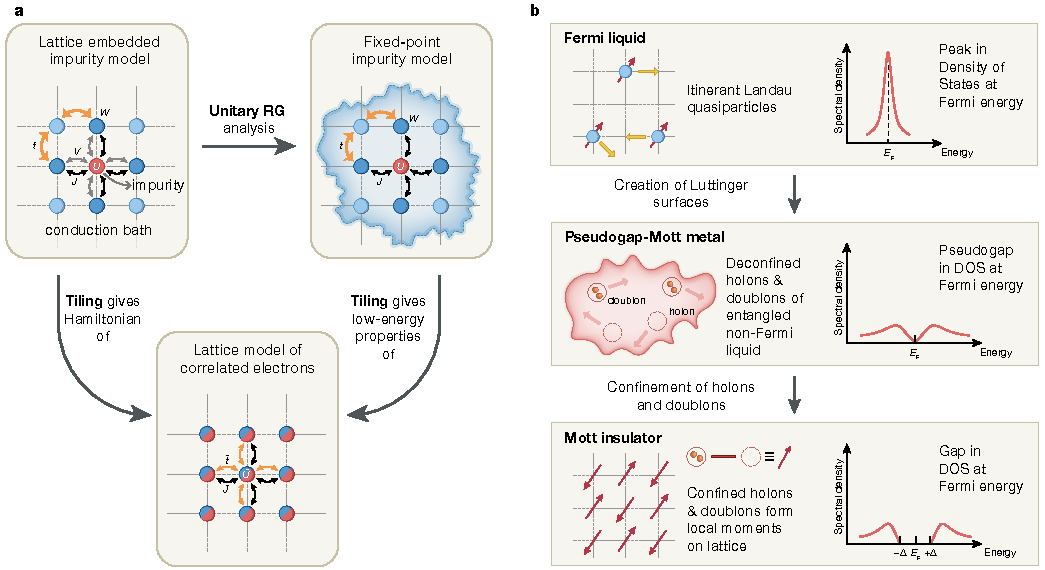
\includegraphics[width=\linewidth]{Figure1_Nature.pdf}
    \caption{Schematic representation of (a) theoretical framework adopted by us (see main text for explanation of symbols), (b) phases obtained for the extended Hubbard model in two dimensions at $T=0$, and passage between them.}
    \label{schematic}
%    \label{schematic:b}
\end{figure*}

Our approach involves developing a renormalization group (RG)-based impurity-to-lattice framework that reconstructs the low-energy physics of a strongly correlated system from the fixed-point structure of a quantum impurity model (Fig.~\hyperref[schematic]{\ref*{schematic}(a)}). Starting from a dynamical Anderson impurity embedded in a correlated bath, we solve the system using a unitary RG (URG) approach~\cite{anirbanurg1,anirbanurg2}. We then construct a translation-invariant lattice Hamiltonian through a many-body tiling procedure that preserves non-local correlations and inherits momentum-resolved self-energies and renormalized couplings from the impurity solution. The resulting model is an \textit{extended}-Hubbard Hamiltonian on a two-dimensional square lattice at half-filling, with both on-site repulsion and nearest-neighbour spin exchange interactions. These correlations, derived directly from the impurity dynamics, enable tracking the evolution from the FL to the Mott insulator (MI) via an intermediate PG phase.

A central insight of our work is that the PG phase hosts a NFL state governed by Kondo frustration and doublon–holon deconfinement~\cite{keimer2015quantum} (Fig.~\hyperref[schematic]{\ref*{schematic}(b)}). A correlation scale ($W$) in the conduction bath suppresses Kondo screening (with coupling $J$) beyond a critical ratio of $W/J$, triggering the emergence of Luttinger surfaces in the lattice model. This breakdown of quasiparticles begins at the antinodes and progressively engulfs the nodal regions, driving a continuous transformation into the MI. The resulting NFL exhibits a pseudogapped density of states that vanishes as $\omega^{2}$ as $\omega \to 0$, multipartite long-range entanglement, and a universal scattering rate of the form $\sim (a + b\,\omega^2)^{-1}$ that grows as $\omega \to 0$. At the critical endpoint of this phase, the URG flow identifies a singular NFL described by the Hatsugai–Kohmoto (HK) model~\cite{Hatsugai1992,Baskaran1991,Huang2022}, with fully deconfined holon–doublon excitations.

The emergence of Luttinger surfaces alters the anomaly structure associated with the generalized symmetry of the FS~\cite{Altshuler_1998,Heath_2020,lanave2025}. The corresponding topological charge is defined via the Luttinger–Ward functional. This charge is modified by Green’s function zeros, signalling a shift in the underlying anomaly. Within our framework, this reorganization grants topological protection to the RG flows terminating in the PG regime, ensuring the stability of its NFL excitations. These are adiabatically connected to the Hatsugai–Kohmoto model~\cite{Hatsugai1992,Baskaran1991}, reinforcing the interpretation of the PG as a distinct quantum phase. We thus identify the NFL state as a new gapless, long-range entangled phase of correlated matter - the \textit{Mott metal} - whose deconfined holon-doublon excitations are eventually confined across the Mott transition~\cite{Mott_1949}.

While we demonstrate our approach for an extended Hubbard model, the underlying framework is broadly applicable to correlated quantum systems. The impurity-plus-tiling construction accommodates multi-orbital degrees of freedom, frustrated geometries, and nontrivial band topology. By deriving lattice Hamiltonians directly from renormalized local dynamics - without relying on mean-field approximations - this method preserves nonlocal correlations and enhances momentum-space resolution. {\color{blue} Coupled with the unitary renormalisation group method as the impurity solver, this approach provides access to one-particle as well as two-particle correlations, entanglement measures and several dynamical quantities, making the method very versatile.} It thus provides a versatile and controlled route for engineering strongly correlated models, particularly in regimes where PG formation, NFL scaling, and Mott physics intersect.

We now describe the layout of the work. In section \ref{auxurgsection}, we formulate the lattice-embedded auxiliary quantum impurity model and sketch the unitary renormalisation group (URG) method employed to analyse the impurity model. In section \ref{tilingsection}, we formulate the tiling procedure by which to map the impurity Hamiltonian, eigenstates and observables into a lattice model of strongly correlated electrons via the usage of many-body translation operators. Section \ref{kondobreakdownsection} displays the destruction of the Fermi liquid from the breakdown of Kondo screening, leading to a pseudogapped non-Fermi liquid phase of matter. The novel properties of this phase are rigorously established in section \ref{NFLproperties}. In section \ref{exactsolforMottCrit}, we demonstrate that the continuous transition between the pseudogap and Mott insulating phases is described by the exactly solvable Hatsugai-Kohmoto model. We demonstrate in section \ref{pseudogapasnovelphase} the universal organising principle that is responsible for the emergence of the pseudogap non-Fermi liquid phase. This also unveils the pseudogap as the strongly coupled long-range entangled parent metal of the Mott insulator. We conclude in section \ref{conclusions}. Finally, we present appendices containing the derivation of the URG analysis of the impurity model, and the exactly solvable model at the critical point.

\section{Auxiliary Model and URG analysis}\label{auxurgsection}
To capture the interplay between Kondo physics and Mott localization, our approach relies on a two-dimensional auxiliary model consisting of an Anderson impurity embedded in a minimally-correlated bath, which we solve the system using a unitary RG (URG) approach~\cite{anirbanurg1,anirbanurg2}. The impurity model and URG analysis are laid out in this section. In order to make contact with a lattice model, we construct a translation-invariant Hamiltonian from the impurity model through a many-body tiling procedure: this preserves non-local correlations, as well as allows for momentum-resolved self-energies and renormalized couplings generated from the impurity solution. For the impurity model chosen in this work, tiling results in an \textit{extended}-Hubbard Hamiltonian on a two-dimensional square lattice at particle-hole symmetry (half-filling). The interaction terms within the lattice model are a result of analogous correlations present in the auxiliary model. This is laid out next in Section~\ref{tilingsection}.

\subsection{Lattice-embedded Impurity Model}
The auxiliary model consists of a correlated impurity site (with a double occupancy cost $U$) embedded within a correlated conduction bath defined on a square lattice (see Fig.~\hyperref[schematic]{\ref*{schematic}(a)}). The impurity site hybridises with the conduction bath sites adjacent to it through one-particle hybridisation $V$ as well as a spin-exchange interaction $J$ arising from fluctuations in local spin densities of the electrons. The conduction bath has minimal correlations in the form of a local correlation term $W$ on the sites that are adjacent to the impurity.

The Hamiltonian of the auxiliary model studied here is
\begin{equation}
\label{impurityModel}
\mathcal{H}_\text{aux} = H_\text{imp} + H_\text{coup} + H_\text{cbath},
\end{equation}
where the particle-hole symmetric impurity term is
\begin{equation}
H_\text{imp} = - \frac{U}{2} \left( \hat{n}_{d \uparrow} - \hat{n}_{d \downarrow} \right)^2,
\label{localrepulsion}
\end{equation}
describing on-site Coulomb interactions at the impurity. Here, $c^\dagger_{d\sigma}$ creates an electron with spin $\sigma$ at the impurity site, and $\hat{n}_{d\sigma} = c^\dagger_{d\sigma} c_{d\sigma}$ denotes the corresponding number operator.

The impurity couples to four nearest-neighbour bath sites $c_{Z\sigma}$ through both hybridization and Kondo exchange:
\begin{equation}\begin{aligned}
H_\text{coup} = \frac{J}{2} \hspace{-0.25cm}\sum_{\sigma_1,\sigma_2,Z} 
%\sum_{Z} 
{\bf S}_d \cdot c^\dagger_{Z\sigma_1} {\boldsymbol \tau}_{\sigma_1 \sigma_2} c_{Z\sigma_2} 
- V \sum_{\sigma,Z} \left( c^\dagger_{Z\sigma} c_{d\sigma} + \text{h.c.} \right),    
\end{aligned}
\label{impbathcoup}\end{equation}
where ${\boldsymbol \tau}$ are the Pauli matrices, and $Z$ indexes the four neighbouring bath sites. The half-filled bath includes nearest neighbour hopping and on-site correlations on the site neighbouring the impurity:
\begin{equation}
H_\text{cbath} = \sum_{\bf k} \epsilon_{\bf k} c^\dagger_{{\bf k},\sigma} c_{{\bf k},\sigma} - \frac{W}{2} \sum_{Z} \left( \hat{n}_{Z\uparrow} - \hat{n}_{Z\downarrow} \right)^2,
\label{bathke}
\end{equation}
where $\epsilon_{\bf k} = -2t(\cos k_x + \cos k_y)$, and $W$ parametrizes local repulsion in the bath that frustrates Kondo screening and drives the system towards local-moment formation. A crucial feature of this construction is that the Kondo coupling acquires a momentum structure upon Fourier transforming:
\begin{equation}
J_{{\bf k}, {\bf k}^\prime} = \frac{J}{2} \left[ \cos(k_x - k^\prime_x) + \cos(k_y - k^\prime_y) \right],
\end{equation}
which respects the $C_4$ symmetry of the square lattice.


\subsection{The unitary renormalisation group method}
In order to obtain the various low-energy phases of our impurity model, we perform a scaling analysis of the associated Hamiltonian using the recently developed unitary renormalisation group (URG) method ~[19,39,40].
%\cite{anirbanurg1,anirbanurg2}. 
The method has been applied successfully on a wide variety of problems of correlated fermions~\cite{santanukagome,1dhubjhep1,anirbanmott1,siddharthacpi,anirban_kondo,Patra_2023}. The method proceeds by resolving quantum fluctuations in high-energy degrees of freedom, leading to a low-energy Hamiltonian with renormalised couplings and new emergent degrees of freedom. Typically, for a system with Fermi energy \(\epsilon_F\) and bandwidth \(E_N\), the sequence of isoenergetic shells \(\left\{E_{(j)}\right\}, E_{j}\in \left[E_0, E_N\right] \) define the states whose quantum fluctuations we sequentially resolve. The momentum states lying on shells \(E_N\) that are far away from the Fermi surface comprise the UV states, while those on shells near the Fermi surface comprise the IR states.

As a result of the URG transformations, the Hamiltonian \(H_{(j)}\) at a given RG step \(j\) involves scattering processes between the \(k-\)states that have energies lower than \(D_{(j+1)}\). The unitary transformation \(U_{(j)}\) is then defined so as to remove the number fluctuations of the currently most energetic set of states \(D_{(j)}\)~\cite{anirbanurg1,anirbanurg2}:
\begin{eqnarray}
	H_{(j-1)} = U_{(j)} H_{(j)} U^\dagger_{(j)}~, \text{such that} ~\left[H_{(j-1)}, \hat n_{j}\right] =0~.
\end{eqnarray}
The eigenvalue of $\hat{n}_{j}$ has, thus, been rendered an integral of motion (IOM) under the RG transformation.

The unitary transformations can be expressed in terms of a generator \(\eta_{(j)}\) that has fermionic algebra~\cite{anirbanurg1,anirbanurg2}:
\begin{eqnarray}
	\label{unitary}
	U_{(j)} = \frac{1}{\sqrt 2}\left(1 + \eta_{(j)} - \eta_{(j)}^\dagger\right)~,~ \quad\left\{ \eta_{(j)},\eta_{(j)}^\dagger \right\} = 1~,
\end{eqnarray}
where \(\left\{\cdot\right\}\) is the anticommutator. The unitary operator \(U_{(j)}\) that appears in Eq.~\eqref{unitary} can be cast into the well-known general form \(U = e^\mathcal{S}, \mathcal{S} = \frac{\pi}{4}\left( \eta^\dagger_{(j)} - \eta_{(j)} \right)\) that a unitary operator can take, defined by an anti-Hermitian operator \(\mathcal{S}\). The generator \(\eta_{(j)}\) is given by the expression\cite{anirbanurg1,anirbanurg2}
\begin{eqnarray}
	\eta^\dagger_{(j)} = \frac{1}{\hat \omega_{(j)} - \text{Tr}\left(H_{(j)} \hat n_{j}\right) } c^\dagger_{j} \text{Tr}\left(H_{(j)}c_{j}\right)~.
\end{eqnarray}
The operators \(\eta_{(j)},\eta^\dagger_{(j)}\) behave as the many-particle analogues of the single-particle field operators \(c_j,c^\dagger_j\) - they change the occupation number of the single-particle Fock space \(\ket{n_j}\).  The important operator \(\hat \omega_{(j)}\) originates from the quantum fluctuations that exist in the problem because of the non-commutation of the kinetic energy terms and the interaction terms in the Hamiltonian:
\begin{eqnarray}
	\hat \omega_{(j)} = H_{(j-1)} - H^i_{(j)}~.
	\label{omega}
\end{eqnarray}
\(H^i_{(j)}\) is the part of \(H_{(j)}\) that commutes with \(\hat n_j\) but does {\it not} commute with at least one \(\hat n_l\) for \(l < j\). The RG flow continues up to energy \(D^*\), where a fixed point is reached from the vanishing of the RG function. 
Detailed comparisons of the URG with other methods (e.g., the functional RG, spectrum bifurcation RG etc.) can be found in Refs.~\cite{anirbanmott1,anirbanurg1}, and implementation on the present problem in  Appendix A.

\section{Derivation of unitary RG equations for the lattice-embedded impurity model}
\subsection{RG scheme}
At any given step \(j\) of the RG procedure, we decouple the states \(\left\{ {\bf q} \right\} \) on the isoenergetic surface of energy \(\varepsilon_j\). The diagonal Hamiltonian \(H_D\) for this step consists of all terms that do not change the occupancy of the states \(\left\{{\bf q}\right\}\):
\begin{equation}\begin{aligned}
	H_D^{(j)} = \varepsilon_j\sum_{q,\sigma}\tau_{q,\sigma} + \frac{1}{2}\sum_{{\bf q}}J_{{\bf q}, {\bf q}}S_d^z\left(\hat n_{{\bf q}, \uparrow} - \hat n_{{\bf q}, \downarrow}\right) - \frac{1}{2}\sum_{{\bf q}}W_{\bf q}\left(\hat n_{{\bf q}, \uparrow} - \hat n_{{\bf q}, \downarrow}\right)^2~,
\end{aligned}\end{equation}
where \(\tau = \hat n - 1/2\) and \(W_{{\bf q}}\) is a shorthand for \(W_{{\bf q},{\bf q},{\bf q},{\bf q}}\). The three terms, respectively, are the kinetic energy of the momentum states on the isoenergetic shell that we are decoupling, the spin-correlation energy between the impurity spin and the spins formed by these momentum states and, finally, the local correlation energy associated with these states arising from the \(W\) term. The off-diagonal part of the Hamiltonian on the other hand leads to scattering in the states \(\left\{ {\bf q} \right\} \). We now list these terms, classified by the coupling they originate from.

\subsubsection*{Arising from the Kondo spin-exchange term}
\begin{equation}\begin{aligned}
	T_{KZ1}^\dagger + T_{KZ1} &= \frac{1}{2}\sum_{{\bf k}, {\bf q}, \sigma}\sigma J_{{\bf k}, {\bf q}} S_d^z  \left[c^\dagger_{{\bf q}\sigma}c_{{\bf k},\sigma} + \text{h.c.}\right],\\
	T_{KZ2}^\dagger + T_{KZ2} &= \frac{1}{2}\sum_{{\bf q}, \sigma}\sigma J_{{\bf q}, {\bf \bar q}} S_d^z  \left[c^\dagger_{{\bf q}\sigma}c_{{\bf \bar q},\sigma} + \text{h.c.}\right],\\
	T_{KT1}^\dagger + T_{KT1} &= \frac{1}{2}\sum_{{\bf k}, {\bf q}}J_{{\bf k}, {\bf q}} \left[S_d^+\left(c^\dagger_{{\bf q}\downarrow}c_{{\bf k}\uparrow} + c^\dagger_{{\bf k}\downarrow}c_{{\bf q}\uparrow}\right) + \text{h.c.}\right],\\
	T_{KT2}^\dagger + T_{KT2} &= \frac{1}{2}\sum_{{\bf q}}J_{{\bf q}, {\bf \bar q}} \left[S_d^+\left(c^\dagger_{{\bf q}\downarrow}c_{{\bf \bar q}\uparrow} + c^\dagger_{{\bf \bar q}\downarrow}c_{{\bf q}\uparrow}\right) + \text{h.c.}\right],\\
\end{aligned}\end{equation}
\subsubsection*{Arising from spin-preserving scattering within conduction bath}
\begin{equation}\begin{aligned}
	T_{P1}^\dagger + T_{P1} &= -\sum_{{\bf q} \in \varepsilon_j}\sum_{{\bf k}_2, {\bf k}_3, {\bf k}_4 < \varepsilon_j}\sum_{\sigma} \left[W_{{\bf q},{\bf k}_2,{\bf k}_3,{\bf k}_4}c^\dagger_{{\bf q},\sigma}c_{{\bf k}_2,\sigma}c^\dagger_{{\bf k}_3,\sigma}c_{{\bf k}_4,\sigma} + \text{h.c.}\right]\\
	T_{P2}^\dagger + T_{P3} &= -\sum_{{\bf q} \in \varepsilon_j}\sum_{{\bf k}_2 < \varepsilon_j}\sum_{\sigma} W_{{\bf q},{\bf k}_2,{\bf \bar q}, {\bf \bar q}} c^\dagger_{{\bf q},\sigma}c_{{\bf k}_2,\sigma} n_{{\bf \bar q},\sigma} -\sum_{{\bf q} \in \varepsilon_j}\sum_{{\bf k}_1 < \varepsilon_j}\sum_{\sigma} W_{{\bf k}_1,{\bf q},{\bf q},{\bf q}} c^\dagger_{{\bf k}_1,\sigma}c_{{\bf q},\sigma} n_{{\bf q},\sigma}\\
	T_{P4} &= -\sum_{{\bf q} \in \varepsilon_j}\sum_{{\bf k}_2, {\bf k}_3 < \varepsilon_j}\sum_{\sigma}W_{{\bf q},{\bf \bar q},{\bf k}_2,{\bf k}_3} c^\dagger_{{\bf q},\sigma}c_{{\bf \bar q},\sigma}c^\dagger_{{\bf k}_2,\sigma}c_{{\bf k}_3,\sigma}\\
	T_{P5} &= -\sum_{{\bf q} \in \varepsilon_j}\sum_{{\bf k}_2, {\bf k}_3 < \varepsilon_j}\sum_{\sigma} W_{{\bf q},{\bf k}_2,{\bf k}_3,{\bf \bar q}} c^\dagger_{{\bf q},\sigma}c_{{\bf k}_2,\sigma}c^\dagger_{{\bf k}_3,\sigma}c_{{\bf \bar q},\sigma}\\
		   &= +\sum_{{\bf q} \in \varepsilon_j}\sum_{{\bf k}_2, {\bf k}_3 < \varepsilon_j}\sum_{\sigma} W_{{\bf q},{\bf k}_3,{\bf k}_2,{\bf \bar q}} c^\dagger_{{\bf q},\sigma}c_{{\bf \bar q},\sigma}c^\dagger_{{\bf k}_2,\sigma}c_{{\bf k}_3,\sigma}\\
		   &= -T_{P4}
\end{aligned}\end{equation}
\subsubsection*{Arising from spin-flip scattering within conduction bath}
\begin{equation}\begin{aligned}
	T_{F1}^\dagger + T_{F1} &= \sum_{{\bf q} \in \varepsilon_j}\sum_{{\bf k}_2, {\bf k}_3, {\bf k}_4 < \varepsilon_j}\sum_{\sigma} \left[W_{{\bf q},{\bf k}_2,{\bf k}_3,{\bf k}_4}c^\dagger_{{\bf q},\sigma}c_{{\bf k}_2,\sigma}c^\dagger_{{\bf k}_3,\bar\sigma}c_{{\bf k}_4,\bar\sigma} + \text{h.c.}\right]\\
	T_{F2} &= \sum_{{\bf q}, {\bf q}^\prime \in \varepsilon_j}\sum_{{\bf k}_2, {\bf k}_3 < \varepsilon_j}\sum_{\sigma}W_{{\bf q},{\bf q}^\prime,{\bf k}_2,{\bf k}_3} c^\dagger_{{\bf q},\sigma}c_{{\bf q}^\prime,\sigma}c^\dagger_{{\bf k}_2,\bar\sigma}c_{{\bf k}_3,\bar\sigma}\\
	T_{F3} &= \sum_{{\bf q}, {\bf q}^\prime \in \varepsilon_j}\sum_{{\bf k}_2, {\bf k}_3 < \varepsilon_j}\sum_{\sigma} W_{{\bf q},{\bf k}_2,{\bf k}_3,{\bf q}^\prime} c^\dagger_{{\bf q},\sigma}c_{{\bf k}_2,\sigma}c^\dagger_{{\bf k}_3,\bar\sigma}c_{{\bf q}^\prime,\bar\sigma} \\
	T_{F4}^\dagger + T_{F4} &= \sum_{{\bf q}, {\bf q}^\prime, \in \varepsilon_j}\sum_{{\bf k}_1 < \varepsilon_j}\sum_{\sigma} \left[W_{{\bf q},{\bf q},{\bf q}^{\prime}, {\bf k}_1} n_{{\bf q},\sigma} c^\dagger_{{\bf q}^{\prime},\bar\sigma}c_{{\bf k}_1,\bar\sigma} + \text{h.c.}\right]
\end{aligned}\end{equation}
In all of the terms \(T_{P[i]}\) and \(T_{F[i]}\), the factor of \(1/2\) in front has been cancelled out by a factor of 2 coming from the multiple possibilities of arranging the momentum labels. We will henceforth ignore \(T_{P4}\) and \(T_{P5}\) because they cancel each other out.

The renormalisation of the Hamiltonian is constructed from the general expression
\begin{equation}\begin{aligned}
	\Delta H^{(j)} = H_X \frac{1}{\omega- H_D} H_X~.
\end{aligned}\end{equation}

The states on the isoenergetic shell \(\pm|\varepsilon_j|\) come in particle-hole pairs \(\left( {\bf q}, {\bf \bar q} \right) \) with energies of opposite signs (relative to the Fermi energy). If \({\bf q}\) is defined as the hole state (unoccupied in the absence of quantum fluctuations), it will have positive energy, while the particle state \({\bf \bar q}\) will be of negative energy and hence below the Fermi surface. To be more specific, given a state \({\bf q}\) with energy \(\pm|\varepsilon_j|\), we define its particle-hole transformed counterpart as the state \({\bf \bar q} = \boldsymbol{\pi} + {\bf q}\), having energy \(\mp|\varepsilon_j|\) and residing in the opposite quadrant of the Brillouin zone. Given this definition, we have the important property that
\begin{equation}\begin{aligned}\label{particleHoleRelation}
	J_{{\bf k}, {\bf \bar q}} &= -J_{{\bf k}, {\bf q}},\\
	W_{\left\{{\bf k}\right\}, {\bf \bar q}} &= -W_{\left\{{\bf k}\right\}, {\bf q}}~.
\end{aligned}\end{equation}

\begin{figure}[htpb]
	\centering
	
\includegraphics[width=0.35\textwidth]{particleHoleRelation.pdf}
	\caption{Particle and hole states.}
	\label{fig:particleHoleRelation-pdf}
\end{figure}
\subsection{Renormalisation of the bath correlation term {\it W}}
The bath correlation term \(W\) can undergo renormalisation only via scattering processes arising from itself. Irrespective of whether the state \({\bf q}\) being decoupled is in a particle or hole configuration in the initial many-body state, the propagator \(G = 1/(\omega - H_D)\) of the intermediate excited state is uniform, and equal to 
\begin{equation}\begin{aligned}\label{propagatorW}
	G_W = 1/\left(\omega - |\varepsilon_j|/2 + W_{\bf q}/2)\right)~,
\end{aligned}\end{equation}
where \(W_{\bf q}\) is the same whether \({\bf q}\) is above or below the Fermi surface. The \(|\varepsilon_j|/2\) in \(H_D\) arises from the excited nature of the state after the initial scattering process.

\subsubsection*{Scattering arising purely from spin-preserving processes}
In this subsection, we calculate the renormalisation to \(W\) arising from the terms \(T_{P1}\), \(T_{P2}\) and \(T_{P3}\). The first term is
\begin{equation}\begin{aligned}
	T_{P1}^\dagger G_W T_{P3} &= \sum_\sigma\sum_{{\bf k}_1, {\bf k}_2, {\bf k}_3, {\bf k}_4} \sum_{\bf q} W_{{\bf q},{\bf k}_2,{\bf k}_3,{\bf k}_4}c^\dagger_{{\bf q},\sigma}c_{{\bf k}_2,\sigma}c^\dagger_{{\bf k}_3,\sigma}c_{{\bf k}_4,\sigma} G_W W_{{\bf k}_1,{\bf q},{\bf q},{\bf q}} c^\dagger_{{\bf k}_1,\sigma}c_{{\bf q},\sigma} n_{{\bf q},\sigma}\\
							  &= -\sum_\sigma\sum_{{\bf k}_1, {\bf k}_2, {\bf k}_3, {\bf k}_4} c^\dagger_{{\bf k}_1,\sigma} c_{{\bf k}_2,\sigma}c^\dagger_{{\bf k}_3,\sigma}c_{{\bf k}_4,\sigma} \sum_{\bf q \in \text{PS}} W_{{\bf q},{\bf k}_2,{\bf k}_3,{\bf k}_4} G_W W_{{\bf k}_1,{\bf q},{\bf q},{\bf q}}~.
\end{aligned}\end{equation}
The operators acting on the states being decoupled contract to form a number operator \(n_{{\bf q},\sigma}\) which projects the sum over \({\bf q}\) into the states that are initial occupied (particle sector, PS). 

The second such contribution is obtained by flipping the sequence of scattering processes:
\begin{equation}\begin{aligned}
	T_{P3} G_W T_{P1}^\dagger &= \sum_\sigma\sum_{{\bf k}_1, {\bf k}_2, {\bf k}_3, {\bf k}_4} \sum_{\bf q} W_{{\bf k}_1,{\bf q},{\bf q},{\bf q}} c^\dagger_{{\bf k}_1,\sigma}c_{{\bf q},\sigma} n_{{\bf q},\sigma} G_W W_{{\bf q},{\bf k}_2,{\bf k}_3,{\bf k}_4}c^\dagger_{{\bf q},\sigma}c_{{\bf k}_2,\sigma}c^\dagger_{{\bf k}_3,\sigma}c_{{\bf k}_4,\sigma} \\
							  &= \sum_\sigma\sum_{{\bf k}_1, {\bf k}_2, {\bf k}_3, {\bf k}_4} c^\dagger_{{\bf k}_1,\sigma} c_{{\bf k}_2,\sigma}c^\dagger_{{\bf k}_3,\sigma}c_{{\bf k}_4,\sigma} \sum_{\bf q \in \text{HS}} W_{{\bf q},{\bf k}_2,{\bf k}_3,{\bf k}_4} G_W W_{{\bf k}_1,{\bf q},{\bf q},{\bf q}}~.
\end{aligned}\end{equation}
By virtue of eq.~\ref{particleHoleRelation}, the product of couplings \(W_{{\bf q},{\bf k}_2,{\bf k}_3,{\bf k}_4} G_W W_{{\bf k}_1,{\bf q},{\bf q},{\bf q}}\) is the same irrespective of whether \({\bf q}\) belongs to the particle or hole sector. The two contributions therefore cancel each other. Moreover, the remaining contributions \(T_{P3}^\dagger G_W T_{P1}\) and \(T_{P1}G_W T_{P2}^\dagger\) are effectively hermitian conjugates of the two contributions considered above, and therefore also cancel each other.

\subsubsection*{Scattering arising from spin-flip processes}
We now come to the processes that involve spin-flips. Considering \(T_{F1}\) and \(T_{F4}\) first, we get
\begin{equation}\begin{aligned}
	T_{F1}^\dagger G_W T_{F4} &= \sum_\sigma\sum_{{\bf k}_1, {\bf k}_2, {\bf k}_3, {\bf k}_4} \sum_{\bf q} W_{{\bf q},{\bf k}_2,{\bf k}_3,{\bf k}_4}c^\dagger_{{\bf q},\sigma}c_{{\bf k}_2,\sigma}c^\dagger_{{\bf k}_3,\bar\sigma}c_{{\bf k}_4,\bar\sigma} G_W W_{{\bf k}_1, {\bf q}, {\bf q}, {\bf q}}  c^\dagger_{{\bf k}_1\sigma} c_{{\bf q}\sigma} n_{{\bf q} \bar \sigma} \\
							  &= -\sum_{1,2,3,4}\sum_\sigma c^\dagger_{{\bf k}_1\sigma} c_{{\bf k}_2\sigma} c^\dagger_{{\bf k}_3\bar\sigma} c_{{\bf k}_4\bar \sigma} \sum_{\bf q \in \text{PS}} W_{{\bf q}, {\bf k}_2, {\bf k}_4, {\bf k}_4} G_W W_{{\bf k}_1, {\bf q}, {\bf q}, {\bf q}}~,\\
	T_{F4} G_W T_{F1}^\dagger &= \sum_\sigma\sum_{{\bf k}_1, {\bf k}_2, {\bf k}_3, {\bf k}_4} \sum_{\bf q}W_{{\bf k}_1, {\bf q}, {\bf q}, {\bf q}}  c^\dagger_{{\bf k}_1\sigma} c_{{\bf q}\sigma} n_{{\bf q} \bar \sigma} G_W W_{{\bf q},{\bf k}_2,{\bf k}_3,{\bf k}_4}c^\dagger_{{\bf q},\sigma}c_{{\bf k}_2,\sigma}c^\dagger_{{\bf k}_3,\bar\sigma}c_{{\bf k}_4,\bar\sigma}  \\
							  &= \sum_{1,2,3,4}\sum_\sigma c^\dagger_{{\bf k}_1\sigma} c_{{\bf k}_2\sigma} c^\dagger_{{\bf k}_3\bar\sigma} c_{{\bf k}_4\bar \sigma} \sum_{\bf q \in \text{HS}} W_{{\bf q}, {\bf k}_2, {\bf k}_4, {\bf k}_4} G_W W_{{\bf k}_1, {\bf q}, {\bf q}, {\bf q}}~.
\end{aligned}\end{equation}
By the same arguments as in the previous subsection, these terms cancel each other out. Their hermitian conjugate contributions \(T_{F1} G_W T_{F4}^\dagger\) and \(T_{F4}^\dagger G_W T_{F1}\) also cancel out. The other two terms are \(T_{F2}\) and \(T_{F3}\), and their contributions also cancel out for the same reason:
\begin{equation}\begin{aligned}
	T_{F2} G_W T_{F2} &= \sum_\sigma\sum_{{\bf k}_1, {\bf k}_2, {\bf k}_3, {\bf k}_4} \sum_{\bf q}W_{{\bf q},{\bf \bar q},{\bf k}_3,{\bf k}_4} c^\dagger_{{\bf q},\sigma}c_{{\bf \bar q},\sigma}c^\dagger_{{\bf k}_3,\bar\sigma}c_{{\bf k}_4,\bar\sigma} G_W W_{{\bf \bar q},{\bf q},{\bf k}_1,{\bf k}_2} c^\dagger_{{\bf \bar q},\sigma}c_{{\bf q},\sigma}c^\dagger_{{\bf k}_1,\bar\sigma}c_{{\bf k}_2,\bar\sigma} \\
							  &= \sum_{1,2,3,4}\sum_\sigma c^\dagger_{{\bf k}_1\sigma} c_{{\bf k}_2\sigma} c^\dagger_{{\bf k}_3\bar\sigma} c_{{\bf k}_4\bar \sigma} \sum_{\bf q \in \text{PS}} W_{{\bf q},{\bf \bar q},{\bf k}_3,{\bf k}_4} G_W W_{{\bf \bar q},{\bf q},{\bf k}_1,{\bf k}_2}~,\\
	T_{F3} G_W T_{F3} &= \sum_\sigma\sum_{{\bf k}_1, {\bf k}_2, {\bf k}_3, {\bf k}_4} \sum_{\bf q} W_{{\bf q},{\bf k}_2,{\bf k}_3,{\bf \bar q}} c^\dagger_{{\bf q},\sigma}c_{{\bf k}_2,\sigma}c^\dagger_{{\bf k}_3,\bar\sigma}c_{{\bf \bar q},\bar\sigma} G_W W_{{\bf \bar q},{\bf k}_4,{\bf k}_1,{\bf q}} c^\dagger_{{\bf \bar q},\bar\sigma} c_{{\bf k}_4,\bar\sigma} c^\dagger_{{\bf k}_1,\sigma} c_{{\bf q},\sigma} \\
							  &= -\sum_{1,2,3,4}\sum_\sigma c^\dagger_{{\bf k}_1\sigma} c_{{\bf k}_2\sigma} c^\dagger_{{\bf k}_3\bar\sigma} c_{{\bf k}_4\bar \sigma} \sum_{\bf q \in \text{PS}} W_{{\bf q},{\bf k}_2,{\bf k}_3,{\bf \bar q}} G_W W_{{\bf \bar q},{\bf k}_4,{\bf k}_1,{\bf q}}~,
\end{aligned}\end{equation}

\subsubsection*{Scattering involving both spin-flip and spin-preserving processes}
These processes involve the combination of terms like \(T_{P1}\) with \(T_{F4}\), and \(T_{P2}\) with \(T_{F1}\). These again cancel each other out for the same reasons as outline above.

\subsubsection*{Net renormalisation for the bath correlation term}
Since all the contributions cancel out in pairs, the bath correlation term \(W\) is {\it marginal}.

\subsection{Renormalisation of the Kondo scattering term {\it J}}
We focus on the renormalisation of the spin-flip part of the Kondo interaction. For these processes, the intermediate many-body state always involves the impurity spin being anti-correlated with the conduction electron spin, such that the propagator for that state is \(G_J = 1/\left(\omega - |\varepsilon_j|/2 + J_{\bf q}/4 + W_{\bf q}/2)\right) \).
\subsubsection*{Impurity-mediated spin-flip scattering purely through Kondo-like processes}
The following processes arising from the Kondo term renormalise the spin-flip interaction:
\begin{equation}\begin{aligned}\label{kondoRenorm1}
	T^\dagger_{KT1} G_J \left(T_{KZ1} + T_{KZ1}^\dagger\right) &= \frac{1}{4}\sum_{{\bf k}_1, {\bf k}_1, {\bf q}}~J_{{\bf q}, {\bf k}_2} S_d^+ \left[-c^\dagger_{{\bf q}\downarrow} c_{{\bf k}_2 \uparrow} G_J c^\dagger_{{\bf k}_1 \downarrow} c_{{\bf q} \downarrow} + c^\dagger_{{\bf k}_2\downarrow} c_{{\bf q} \uparrow} G_J c^\dagger_{{\bf q}\uparrow} c_{{\bf k}_1 \uparrow}\right]J_{{\bf k}_1,{\bf q}} S_d^z\\
								&= -\frac{1}{8}\sum_{{\bf k}_1, {\bf k}_1, {\bf q}}~J_{{\bf q}, {\bf k}_2} S_d^+ \left[ c^\dagger_{{\bf k}_1 \downarrow}c_{{\bf k}_2 \uparrow} G_J n_{{\bf q} \downarrow} + c^\dagger_{{\bf k}_2\downarrow} c_{{\bf k}_1 \uparrow}(1 - n_{{\bf q} \uparrow}) G_J \right]J_{{\bf k}_1,{\bf q}}\\
								&= -\frac{1}{8}\sum_{{\bf k}_1, {\bf k}_1}~ S_d^+ c^\dagger_{{\bf k}_1 \downarrow}c_{{\bf k}_2 \uparrow}\sum_{{\bf q} \in \text{PS}}\left[J_{{\bf q}, {\bf k}_2} J_{{\bf k}_1,{\bf q}} + J_{{\bf \bar q}, {\bf k}_1} J_{{\bf k}_2,{\bf \bar q}} \right]G_J~.
\end{aligned}\end{equation}
In getting the final expression, we used the sigma matrix relation \(S_d^+ S_d^z = -\frac{1}{2}S_d^+\), and absorbed the projector \(1 - n_{{\bf q} \uparrow}\) into the sum over the particle sector by replacing \(q\) with its particle-hole transformed counterpart \(\bar q\). An identical contribution is obtained by switching the sequence of processes:
\begin{equation}\begin{aligned}\label{kondoRenorm2}
	 \left(T_{KZ1} + T_{KZ1}^\dagger\right) G_J T^\dagger_{KT1} &= \frac{1}{4}\sum_{{\bf k}_1, {\bf k}_1, {\bf q}}~J_{{\bf k}_1,{\bf q}} S_d^z\left[- c^\dagger_{{\bf k}_1 \downarrow} c_{{\bf q} \downarrow}G_J c^\dagger_{{\bf q}\downarrow} c_{{\bf k}_2 \uparrow} +c^\dagger_{{\bf q}\uparrow} c_{{\bf k}_1 \uparrow} G_J c^\dagger_{{\bf k}_2\downarrow} c_{{\bf q} \uparrow} \right] J_{{\bf q}, {\bf k}_2} S_d^+ \\
								&= -\frac{1}{8}\sum_{{\bf k}_1, {\bf k}_1}~ S_d^+ c^\dagger_{{\bf k}_1 \downarrow}c_{{\bf k}_2 \uparrow}\sum_{{\bf q} \in \text{PS}}\left[J_{{\bf \bar q}, {\bf k}_2} J_{{\bf k}_1,{\bf \bar q}} + J_{{\bf q}, {\bf k}_1} J_{{\bf k}_2,{\bf q}} \right]G_J~.
\end{aligned}\end{equation}

\subsubsection*{Scattering processes involving interplay between the Kondo interaction and conduction bath interaction}
Looking at \(T_{KT1}^\dagger\) first, we have
\begin{equation}\begin{aligned}\label{t7t6}
	T_{KT1}^\dagger G_J \left(T_{F4} + T_{F4}^\dagger\right) &= \frac{1}{2}\sum_{{\bf k}_1,{\bf k}_2,{\bf q}} J_{{\bf k}_2, {\bf q}}S_d^+ \left(c^\dagger_{{\bf q}\downarrow}c_{{\bf k}_2\uparrow}  G_J W_{{\bf q}, {\bf q}, {\bf k}_1, {\bf q}} n_{q \uparrow} c^\dagger_{{\bf k}_1 \downarrow} c_{{\bf q} \downarrow} + c^\dagger_{{\bf k}_2\downarrow}c_{{\bf q}\uparrow}  G_J W_{{\bf \bar q}, {\bf \bar q}, {\bf q}, {\bf k}_1} n_{\bar q \downarrow} c^\dagger_{{\bf q} \uparrow} c_{{\bf k}_1 \uparrow}\right) ~.
\end{aligned}\end{equation}
For either of the two choices of the functional form of \(W\), it is easy to show that \(W_{{\bf q}, {\bf q}, {\bf k}_1, {\bf q}} = W_{{\bf \bar q}, {\bf \bar q}, {\bf q}, {\bf k}_1}\).
\begin{equation}\begin{aligned}\label{KT1F4}
	T_{KT1}^\dagger G_J \left(T_{F4} + T_{F4}^\dagger\right) &= \frac{1}{2}\sum_{{\bf k}_1,{\bf k}_2,{\bf q}} J_{{\bf k}_2, {\bf q}} W_{{\bf q}, {\bf q}, {\bf k}_1, {\bf q}} G_J S_d^+ \left[-c^\dagger_{{\bf k}_1 \downarrow}c_{{\bf k}_2\uparrow} n_{{\bf q}\downarrow} n_{q \uparrow} + c^\dagger_{{\bf k}_2\downarrow} c_{{\bf k}_1 \uparrow} (1 - n_{{\bf q}\uparrow}) n_{\bar q \downarrow}\right] ~.
\end{aligned}\end{equation}

Another contribution is obtained by switching the sequence of the scattering processes:
\begin{equation}\begin{aligned}\label{F4KT1}
	\left(T_{F4} + T_{F4}^\dagger\right) G_J T_{KT1}^\dagger &= \frac{1}{2}\sum_{{\bf k}_1,{\bf k}_2,{\bf q}} \left(W_{{\bf q}, {\bf q}, {\bf k}_1, {\bf q}} n_{\bar q \uparrow} c^\dagger_{{\bf k}_1 \downarrow} c_{{\bf q} \downarrow} G_J c^\dagger_{{\bf q}\downarrow}c_{{\bf k}_2\uparrow} + W_{{\bf \bar q}, {\bf \bar q}, {\bf q}, {\bf k}_1} n_{q \downarrow} c^\dagger_{{\bf q} \uparrow} c_{{\bf k}_1 \uparrow} G_J c^\dagger_{{\bf k}_2\downarrow}c_{{\bf q}\uparrow} \right) J_{{\bf k}_2, {\bf q}}S_d^+\\
															 &= \frac{1}{2}\sum_{{\bf k}_1,{\bf k}_2,{\bf q}} \left(c^\dagger_{{\bf k}_1 \downarrow} c_{{\bf k}_2\uparrow} n_{\bar q \uparrow} (1 - n_{{\bf q} \downarrow}) - c^\dagger_{{\bf k}_2\downarrow}c_{{\bf k}_1 \uparrow}n_{q \downarrow} n_{{\bf q} \uparrow}\right) W_{{\bf q}, {\bf q}, {\bf k}_1, {\bf q}} G_J J_{{\bf k}_2, {\bf q}}S_d^+
\end{aligned}\end{equation}
The two contributions (eqs.~\ref{KT1F4} and \ref{F4KT1}) arising from \(T_{KT1}\) cancel each other.

We now consider the other spin-exchange process \(T_{KT2}^\dagger\). One such contribution is
\begin{equation}\begin{aligned}\label{kondoRenorm3}
	T_{KT2}^\dagger G_J T_{F3} &= \frac{1}{2}\sum_{{\bf k}_1,{\bf k}_2,{\bf q}} J_{{\bf q}, {\bf \bar q}}S_d^+ \left(c^\dagger_{{\bf q}\downarrow}c_{{\bf \bar q}\uparrow} G_J c^\dagger_{{\bf \bar q} \uparrow} c_{{\bf k}_2 \uparrow} c^\dagger_{{\bf k}_1 \downarrow} c_{{\bf q} \downarrow} + c^\dagger_{{\bf \bar q}\downarrow}c_{{\bf q}\uparrow}  G_J  c^\dagger_{{\bf q} \uparrow} c_{{\bf k}_2 \uparrow} c^\dagger_{{\bf k}_1 \downarrow} c_{{\bf \bar q} \downarrow}\right)W_{{\bf \bar q}, {\bf k}_2, {\bf k}_1, {\bf q}}\\
							   &= -\frac{1}{2}\sum_{{\bf k}_1,{\bf k}_2,{\bf q}} S_d^+ c^\dagger_{{\bf k}_1 \downarrow} c_{{\bf k}_2 \uparrow}\left[n_{{\bf q}\downarrow}(1 - n_{{\bf \bar q}\uparrow}) + n_{{\bf \bar q}\downarrow}(1 - n_{{\bf q}\uparrow}) \right] J_{{\bf q}, {\bf \bar q}} G_J W_{{\bf \bar q}, {\bf k}_2, {\bf k}_1, {\bf q}}\\
							   &= -\frac{1}{2}\sum_{{\bf k}_1,{\bf k}_2} S_d^+ c^\dagger_{{\bf k}_1 \downarrow} c_{{\bf k}_2 \uparrow}\sum_{{\bf q} \in \text{PS}}\left(J_{{\bf q}, {\bf \bar q}} W_{{\bf \bar q}, {\bf k}_2, {\bf k}_1, {\bf q}} + J_{{\bf \bar q}, {\bf q}} W_{{\bf q}, {\bf k}_2, {\bf k}_1, {\bf \bar q}}\right)G_J~.
\end{aligned}\end{equation}
An identical contribution is obtained from the reversed term:
\begin{equation}\begin{aligned}\label{kondoRenorm4}
	T_{F3}G_J T_{KT2}^\dagger  &= \frac{1}{2}\sum_{{\bf k}_1,{\bf k}_2,{\bf q}} W_{{\bf \bar q}, {\bf k}_2, {\bf k}_1, {\bf q}}\left(c^\dagger_{{\bf \bar q} \uparrow} c_{{\bf k}_2 \uparrow} c^\dagger_{{\bf k}_1 \downarrow} c_{{\bf q} \downarrow} G_J c^\dagger_{{\bf q}\downarrow}c_{{\bf \bar q}\uparrow} +  c^\dagger_{{\bf q} \uparrow} c_{{\bf k}_2 \uparrow} c^\dagger_{{\bf k}_1 \downarrow} c_{{\bf \bar q} \downarrow} G_J c^\dagger_{{\bf \bar q}\downarrow}c_{{\bf q}\uparrow} \right)J_{{\bf q}, {\bf \bar q}}S_d^+ \\
							   &= -\frac{1}{2}\sum_{{\bf k}_1,{\bf k}_2} S_d^+ c^\dagger_{{\bf k}_1 \downarrow} c_{{\bf k}_2 \uparrow}\sum_{{\bf q} \in \text{PS}}\left(J_{{\bf q}, {\bf \bar q}} W_{{\bf \bar q}, {\bf k}_2, {\bf k}_1, {\bf q}} + J_{{\bf \bar q}, {\bf q}} W_{{\bf q}, {\bf k}_2, {\bf k}_1, {\bf \bar q}}\right)G_J~.
\end{aligned}\end{equation}

\subsubsection*{Net renormalisation to the Kondo interaction}
Combining the results from eqs.~\ref{kondoRenorm1}, \ref{kondoRenorm2}, \ref{kondoRenorm3} and \ref{kondoRenorm4}, as well as using the properties \(J_{{\bf \bar q}, {\bf k}_1} J_{{\bf k}_2,{\bf \bar q}} = J_{{\bf q}, {\bf k}_2} J_{{\bf k}_1,{\bf q}} = J_{{\bf k}_2, {\bf q}} J_{{\bf q},{\bf k}_1}\) and \(J_{{\bf q}, {\bf \bar q}} W_{{\bf \bar q}, {\bf k}_2, {\bf k}_1, {\bf q}} = J_{{\bf \bar q}, {\bf q}} W_{{\bf q}, {\bf k}_2, {\bf k}_1, {\bf \bar q}}\), the total renormalisation in the momentum-resolved Kondo coupling \(J^{(j)}\) at the \(j^\text{th}\) step amounts to
\begin{equation}\begin{aligned}
	\Delta J^{(j)}_{{\bf k}_1, {\bf k}_2} = -\sum_{{\bf q} \in \text{PS}} \frac{J^{(j)}_{{\bf k}_2,{\bf q}} J^{(j)}_{{\bf q},{\bf k}_1} + 4J^{(j)}_{{\bf q}, {\bf \bar q}} W_{{\bf \bar q}, {\bf k}_2, {\bf k}_1, {\bf q}}}{\omega - \frac{1}{2}|\varepsilon_j| + J^{(j)}_{{\bf q}}/4 + W_{{\bf q}}/2}
\end{aligned}\end{equation}

A representation of the RG phase diagram in the $-W/t$ vs. $J/t$ plane of couplings has been provided in Fig.\hyperref[spinCorr]{\ref*{spinCorr}(a)} from detailed numerical computations of eq.\eqref{rgeq2}. We also provide a schematic representation of RG flows to various fixed point theories in the $J$ vs. $W$ plane of couplings in Fig.\ref{rgflows}. This schematic figure shows the existence of three distinct phases (Fermi liquid metal, Mott Insulator, and Pseudogap-Mott metal) described by distinct fixed point theories of the RG flows. The Fermi liquid metal and Mott Insulator phases are distinguished from the Pseudogap-Mott metal by separatrices of the RG flows.
\begin{figure}
    \centering
    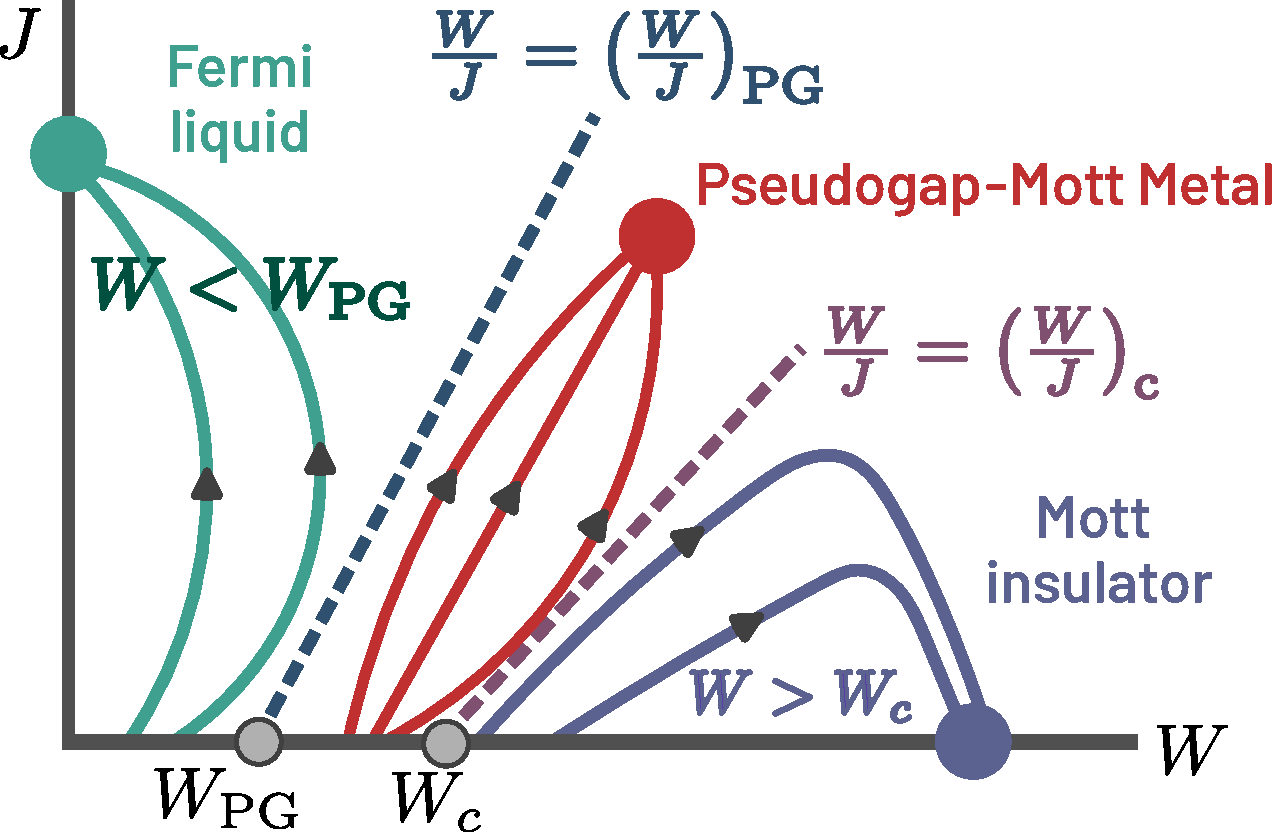
\includegraphics[width=0.5\linewidth]{RGflows.pdf}
    \caption{Renormalisation group (RG) flow diagram of the lattice model as obtained from a unitary RG analysis of the lattice-embedded impurity model. For $|W/J| < |W/J|_\text{PG}$, the flows lead to a Fermi liquid phase, while for $|W/J| < |W/J|_\text{c}$, they lead to a Mott insulator. For values in between, the system flows to a Mott metal phase that has a pseudogap in the density of states.}
    \label{rgflows}
\end{figure}
\begin{figure*}
    \centering
    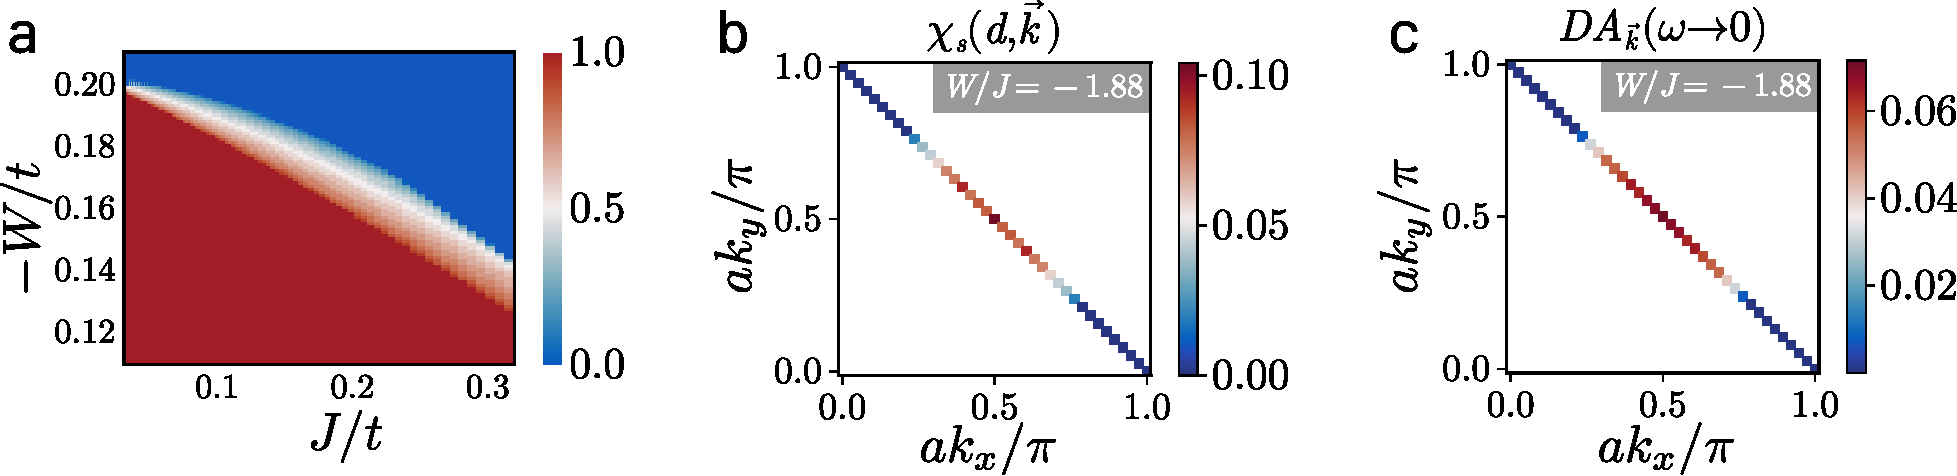
\includegraphics[width=\textwidth]{fig2.pdf}
    \caption{(a) Phase diagram of impurity model at strong coupling in $U$ in terms of competing dimensionless Kondo ($J/t$) and bath correlation ($W/t$) couplings. Colourbar represents the fraction of states on the Fermi surface replaced by zeros of the Greens function (Luttinger surface). A pseudogap phase (shaded region) is observed between the local Fermi liquid (red region) and local moment (blue region) phases (b) $k$-space-resolved spin-spin correlation $\chi_s(d,{\bf k}) = \braket{{\bf S}_d\cdot{\bf S}_{\bf k}}$ in the pseudogap phase of the impurity model. Antinodal regions are observed to decouple from Kondo screening of the impurity. (c) Upon tiling, this leads to a $k$-space-resolved antinodal gap in the electronic density of states of the lattice model, corresponding to Luttinger surfaces of zeros.}
    \label{spinCorr}
%    \label{spinCorr:b}
%    \label{spinCorr:c}
\end{figure*}

\begin{figure}[!th]
    \centering
    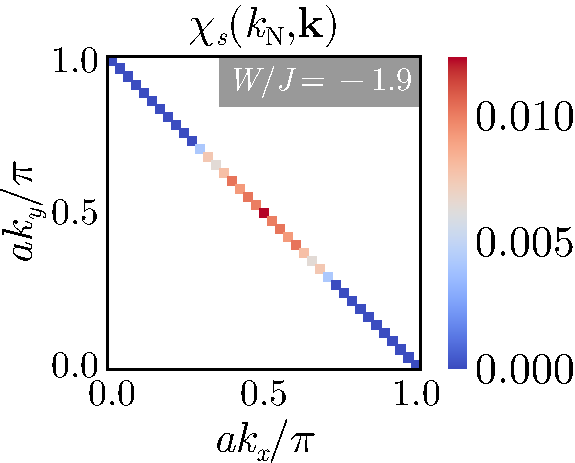
\includegraphics[width=0.49\linewidth]{tiled-SF-3.pdf}
    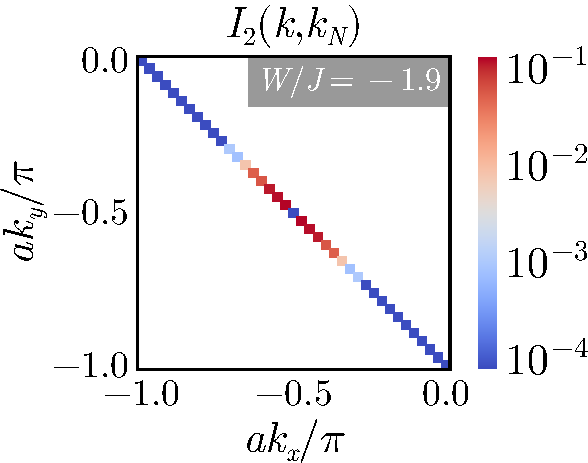
\includegraphics[width=0.49\linewidth]{tiled_I2_k_N_2000-3.pdf}
    \caption{Left: Spin correlations \(\chi_s\) for the {\it tiled model}, between the nodal point \(k_N = \left( -\pi/2, -\pi/2\right)\) and an arbitrary \(k-\)point on the Fermi surface. In the PG, the spin-correlations near the antinode vanish, indicating that they have been removed from the metallic excitations, while the correlations near the nodal point become enhanced because of the increasingly correlated nature of the metal. Right: Mutual information \(I_2\) between an arbitrary \(k-\)state and the nodal point. The nodal points remain strongly entangled with each other all the way through the PG.}
    \label{tiledEntanglement}
\end{figure}

\begin{figure*}[!th]
    \centering
    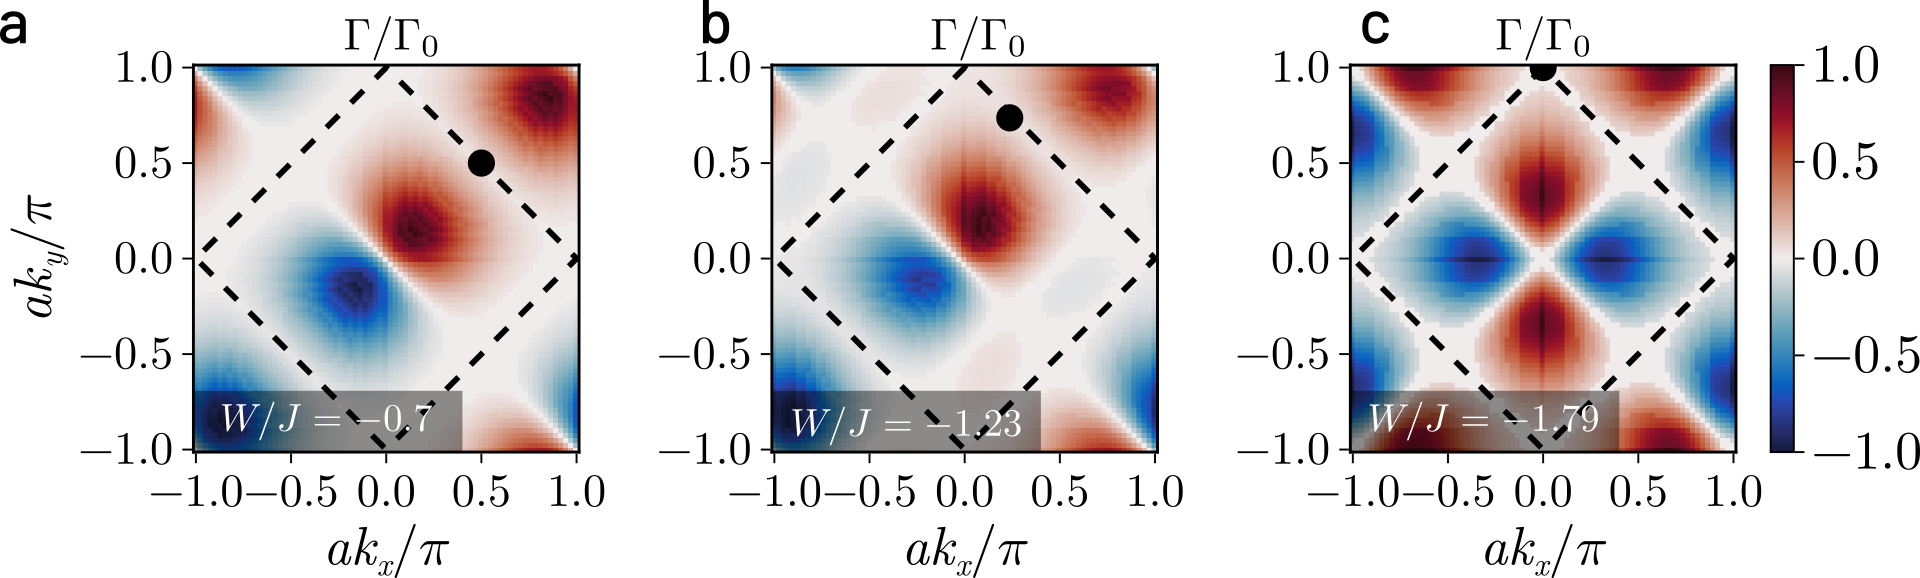
\includegraphics[width=\textwidth]{fig2.5.png}
    \caption{Initiation of the decoupling of $J_{{\bf k}, {\bf k'}}$ (positive, negative and zeros shown in red, blue and white respectively), with ${\bf k}$ (black circle) at low-energies for ${\bf k}$ corresponding to the node (a), antinode (b) and a point mid-way between them (c) on the top right arm of the FS respectively with tuning $W/J$. As dictated by the symmetry of $J_{{\bf k}, {\bf k'}}$, the decoupling for a given ${\bf k}$ proceeds via the appearance of zeros (white patches) of $J_{{\bf k}, {\bf k'}}$ for ${\bf k'}$ initially on the nodal regions of adjacent arms, and progresses gradually towards the antinodes. The decoupling ends with the onset of the pseudogap.}
    \label{unravelling}
%    \label{unravelling:b}
%    \label{unravelling:c}
\end{figure*}

\section{Reconstructing of lattice model from auxiliary model}
To reconstruct a translationally invariant lattice Hamiltonian from the impurity model (with Hamiltonian $\mathcal{H}_\text{aux}$), we define a many-body tiling prescription that embeds the auxiliary impurity system uniformly across the two-dimensional square lattice. Thus, the tiling process systematically derives the full lattice dynamics from the renormalized fixed-point structure of the impurity. As described in Section~\ref{auxurgsection}, the auxiliary model consists of a single impurity embedded in a correlated bath at the location $\mathbf{r}_d$: 
\begin{equation}
H(\mathbf{r}_d) = H_{\text{imp}} + H_{\text{cbath}} + H_{\text{imp-cbath}}~.
\label{auxmodel}
\end{equation}
The form of various terms in eq.\eqref{auxmodel}
have been defined in eqs.\eqref{localrepulsion}, \eqref{impbathcoup} and \eqref{bathke} in Section~\ref{auxurgsection}.
% where the impurity, conduction bath and impurity–bat Hamiltonians are defined as
% \begin{equation}
% \begin{aligned}
% H_{\text{imp}} &= -\frac{U}{2} \left( \hat{n}_{\mathbf{r}_d\uparrow} - \hat{n}_{\mathbf{r}_d\downarrow} \right)^2,\\
% H_{\text{cbath}} &= -\frac{1}{\sqrt{\mathcal{Z}}} t \sum_{\langle \mathbf{r}_i, \mathbf{r}_j \rangle \ne \mathbf{r}_d; \sigma} \left( c^\dagger_{\mathbf{r}_i\sigma} c_{\mathbf{r}_j\sigma} + \text{h.c.} \right) \\
% &- \frac{1}{2\mathcal{Z}} W \sum_{\mathbf{z} \in \text{NN}(\mathbf{r}_d)} \left( \hat{n}_{\mathbf{z}\uparrow} - \hat{n}_{\mathbf{z}\downarrow} \right)^2,\\
% H_{\text{imp-cbath}} &= \frac{J}{\mathcal{Z}} \sum_{\sigma, \sigma'} \sum_{\mathbf{z} \in \text{NN}(\mathbf{r}_d)} \mathbf{S}_{\mathbf{r}_d} \cdot \boldsymbol{\tau}_{\sigma \sigma'} c^\dagger_{\mathbf{z}\sigma} c_{\mathbf{z}\sigma'} \\
% &- \frac{V}{\sqrt{\mathcal{Z}}} \sum_{\sigma} \sum_{\mathbf{z} \in \text{NN}(\mathbf{r}_d)} \left( c^\dagger_{\mathbf{r}_d\sigma} c_{\mathbf{z}\sigma} + \text{h.c.} \right).
% \end{aligned}
% \end{equation}
% $\boldsymbol{\tau} = (\tau_x, \tau_y, \tau_z)$ are Pauli matrices, and ${\bf r}_d$ denotes the impurity position.

The tiled lattice Hamiltonian is generated by symmetrically translating this impurity model:
\begin{equation}
\mathcal{H}_{\text{tiled}} = \mathcal{T}[H(\mathbf{r}_d)] = \sum_{\mathbf{r}} T^\dagger(\mathbf{r} - \mathbf{r}_d) H(\mathbf{r}_d) T(\mathbf{r} - \mathbf{r}_d),
\end{equation}
where $T(\mathbf{a})$ are many-body translation operators~\cite{stoyanova}:
\begin{equation}
T^\dagger(\mathbf{a}) \mathcal{O}(\{\mathbf{r}_i\}) T(\mathbf{a}) = \mathcal{O}(\{\mathbf{r}_i + \mathbf{a}\}).
\end{equation}
Applying this to each term yields:
\begin{equation}\hspace{-0.5cm}\begin{aligned}
\mathcal{T}[H_{\text{cbath}}] &= -\frac{(N - 2)t}{\sqrt{\mathcal{Z}}} \sum_{\langle \mathbf{r}_i, \mathbf{r}_j \rangle; \sigma} \left( c^\dagger_{\mathbf{r}_i\sigma} c_{\mathbf{r}_j\sigma} + \text{h.c.} \right) \\
&- \frac{1}{2} W \sum_{\mathbf{r}} \left( \hat{n}_{\mathbf{r}\uparrow} - \hat{n}_{\mathbf{r}\downarrow} \right)^2, \\
\mathcal{T}[H_{\text{imp}}] &= -\frac{U}{2} \sum_{\mathbf{r}} \left( \hat{n}_{\mathbf{r}\uparrow} - \hat{n}_{\mathbf{r}\downarrow} \right)^2, \\
\mathcal{T}[H_{\text{imp-cbath}}] &= \sum_{\langle \mathbf{r}_i, \mathbf{r}_j \rangle} \left[ \frac{2J}{\mathcal{Z}} \mathbf{S}_{\mathbf{r}_i} \cdot \mathbf{S}_{\mathbf{r}_j} - \frac{2V}{\sqrt{\mathcal{Z}}} \sum_\sigma \left( c^\dagger_{\mathbf{r}_i\sigma} c_{\mathbf{r}_j\sigma} + \text{h.c.} \right) \right],
\end{aligned}\end{equation}
with local spin operators defined as
\begin{equation}
\mathbf{S}_{\mathbf{r}} = \sum_{\sigma, \sigma'} c^\dagger_{\mathbf{r}\sigma} \boldsymbol{\tau}_{\sigma \sigma'} c_{\mathbf{r}\sigma'}.
\end{equation}

To avoid overcounting of the non-interacting bath terms, we subtract extra copies of the kinetic energy term. The reconstructed extended–Hubbard model then reads:
\begin{equation}
\begin{aligned}
\mathcal{H}_{\text{tiled}} = & -\frac{1}{\sqrt{\mathcal{Z}}} \tilde{t} \sum_{\langle \mathbf{r}_i, \mathbf{r}_j \rangle; \sigma} \left( c^\dagger_{\mathbf{r}_i\sigma} c_{\mathbf{r}_j\sigma} + \text{h.c.} \right) \\
&+ \frac{\tilde{J}}{\mathcal{Z}} \sum_{\langle \mathbf{r}_i, \mathbf{r}_j \rangle} \mathbf{S}_{\mathbf{r}_i} \cdot \mathbf{S}_{\mathbf{r}_j} - \frac{1}{2} \tilde{U} \sum_{\mathbf{r}} \left( \hat{n}_{\mathbf{r}\uparrow} - \hat{n}_{\mathbf{r}\downarrow} \right)^2,
\end{aligned}
\end{equation}
where the effective lattice couplings are given by:
\begin{equation}
\tilde{t} = t + 2V,\quad \tilde{U} = U + W,\quad \tilde{J} = 2J.
\end{equation}
% \end{widetext}

A non-zero chemical potential in the bath and/or the impurity can be included to study the effects of doping. Crucially, the eigenstates of $\mathcal{H}_\text{tiled}$ obey a many-body generalization of Bloch’s theorem~\cite{stoyanova}, which allows for the exact computation of momentum-resolved observables (presented here for a $77\times 77$ {\bf k}-space Brillouin zone grid). We shall demonstrate below that the lattice embedding and tiling procedures provide a controlled route to capture low-energy NFL behavior and Mott criticality directly from a quantum impurity model.

\section{Effective action for the Hubbard-Heisenberg model and the eSIAM}
In order to better understand the similarities and differences between the tiling approach outlined here and the approach adopted in dynamical mean-field approximations, we compute the effective action for the local impurity as well as the impurity-zeroth site system, in both the auxiliary and bulk models. This will be done in the limit of infinite coordination number, in order to create a tractable effective theory.

\subsection{Local theory for the Hubbard-Heisenberg model}
We will first work with the Hubbard-Heisenberg model. Let us recall that within the eSIAM, most of the dynamics is governed by the physics of the impurity site and the bath site coupled to the impurity. Accordingly, we will first obtain an effective action within the Hubbard-Heisenberg model for the small system consisting of a local site and all its nearest-neighbours. 

We choose a certain local site that we call \(0\), whose nearest-neighbours will be denoted as \(\left\{ {\bar 0} \right\} \). The action for the full Hubbard-Heisenberg model can be formally separated into three parts:
\begin{equation}\begin{aligned}
S_\text{H-H} = S_{0,{\bar 0}} + S^{(0,{\bar 0})} + S_\text{int}~,
\end{aligned}\end{equation}
where \(S_{0,{\bar 0}}\) represents the part of the action that involves only the sites \(0\) and $\left\{ {\bar 0} \right\}$, \(S^{(0,{\bar 0})}\) represents the part that has all the sites apart from \(0\) and \(\left\{ {\bar 0} \right\} \), while \(S_\text{int}\) contains all terms that connect these two parts. These three parts have the forms
\begin{equation}\begin{aligned}
S_{0,{\bar 0}} = \sum_{i=0,{\bar 0}}\sum_\sigma \int_0^\beta\mathrm{d\tau}~c^\dagger_{i\sigma}(\tau)\partial_\tau c_{i\sigma}(\tau)  - t\sum_{{\bar 0},\sigma}\int_0^\beta\mathrm{d\tau}~\left[c^\dagger_{0\sigma}(\tau)c_{{\bar 0}\sigma}(\tau) + \text{h.c.}\right] \\
- \frac{U}{2}\sum_{i=0,{\bar 0}}\int_0^\beta\mathrm{d\tau}~\left(n_{i \uparrow}(\tau) - n_{i \downarrow}(\tau)\right)^2 + J\sum_{{\bar 0}}\int_0^\beta\mathrm{d\tau} \vec{S}_0(\tau)\cdot\vec{S}_{{\bar 0}}(\tau)~,
\end{aligned}\end{equation}
\begin{equation}\begin{aligned}
S^{(0,{\bar 0})} = \sum_{j\neq(0,{\bar 0})}\sum_\sigma \int_0^\beta\mathrm{d\tau}~c^\dagger_{j\sigma}(\tau)\partial_\tau c_{j\sigma}(\tau)  - t\sum_{\left<j,l\right>\neq (0,{\bar 0}),\sigma}\int_0^\beta\mathrm{d\tau}~\left[c^\dagger_{j\sigma}(\tau)c_{l\sigma}(\tau) + \text{h.c.}\right] \\
- \frac{U}{2}\sum_{j\neq(0,{\bar 0})}\int_0^\beta\mathrm{d\tau}~\left(n_{j\uparrow}(\tau) - n_{j\downarrow}(\tau)\right)^2 + J\sum_{\left<j,l\right>\neq(0,{\bar 0})}\int_0^\beta\mathrm{d\tau} \vec{S}_l(\tau)\cdot\vec{S}_j(\tau)~,
\end{aligned}\end{equation}
\begin{equation}\begin{aligned}
S_\text{int} = -t\sum_{i \in {\bar 0}}\sum_{j \in \text{NN of}~i}\sum_\sigma \int_0^\beta\mathrm{d\tau}~\left(c^\dagger_{i\sigma}(\tau) c_{j\sigma}(\tau) + \text{h.c.}\right) + J\sum_{i \in {\bar 0}}\sum_{j \in \text{NN of}~i}\int_0^\beta\mathrm{d\tau}\vec{S}_i(\tau)\cdot\vec{S}_j(\tau) = S_\text{int}^\text{hop} + S_\text{int}^\text{spin} 
\end{aligned}\end{equation}

In order to obtain an effective theory \(S^{0,{\bar 0}}_\text{eff}\) purely for the local system \((0,{\bar 0})\), we need to trace over all the other degrees of freedom. This partial trace will be carried out over the states of the so-called ``cavity" system \(S^{(0,{\bar 0})}\). The effective action can be constructed by tracing over scattering processes of all orders that leave the final action diagonal in the system \((0,{\bar 0})\). The formal expression can be written as
\begin{equation}\begin{aligned}
	S^{0,{\bar 0}}_\text{eff} = S_{0,{\bar 0}} + \sum_{n=1}^\infty \braket{\left(S_\text{int}^\text{hop}\right)^{2n}}_{(0,{\bar 0})} + \sum_{n=1}^\infty \braket{\left(S_\text{int}^\text{spin}\right)^{2n}}_{(0,{\bar 0})}
\end{aligned}\end{equation}
where, as mentioned before, the average is carried out in the cavity system \(S^{(0,{\bar 0})}\). Each hopping term in the expansion is of the form
\begin{equation}\begin{aligned}
	\left(S_\text{int}^\text{hop}\right)^{2n} =& t^{2n}\sum_\sigma\sum_{(i_1, i_1^\prime)\ldots, (i_n, i_n^\prime)} ~\sum_{(j_1, j_1^\prime)\ldots, (j_n, j_n^\prime)} \int_0^\beta d\tau_{1}\ldots d\tau_{n}d\tau_{1}^\prime\ldots d\tau_{j_n}^\prime\\
			   &c^\dagger_{i_1\sigma}(\tau_{i_1})c^\dagger_{i_2\sigma}(\tau_{2})\ldots c^\dagger_{i_n\sigma}(\tau_{n}) c_{i_1^\prime\sigma}(\tau_{1}^\prime)c_{i_2^\prime\sigma}(\tau_{2}^\prime)\ldots c_{i_n^\prime\sigma}(\tau_{n}^\prime)\left<c_{j_1\sigma}(\tau_{1})c_{j_2\sigma}(\tau_{2})\ldots c_{j_n\sigma} ~ c^\dagger_{j_1^\prime\sigma}(\tau_{1}^\prime)\ldots c^\dagger_{j_n^\prime\sigma}(\tau_{n}^\prime) \right>_{(0,{\bar 0})}\\
	=& t^{2n}\sum_\sigma\sum_{(i_1, i_1^\prime)\ldots, (i_n, i_n^\prime)} ~\sum_{(j_1, j_1^\prime)\ldots, (j_n, j_n^\prime)} \int_0^\beta d\tau_{1}\ldots d\tau_{j_n}^\prime c^\dagger_{i_1\sigma}(\tau_{i_1})\ldots c^\dagger_{i_n\sigma}(\tau_{n})~c_{i_1^\prime\sigma}(\tau_{1}^\prime)\ldots c_{i_n^\prime\sigma}(\tau_{n}^\prime)\\
	 &G_n^{(0,\bar 0)}\left(\tau_1\ldots \tau_n; \tau_1^\prime\ldots \tau_n^\prime\right)~,
\end{aligned}\end{equation}
where the indices \(i_1\) through \(i_n\) and their primed counterparts run through \(\bar 0\), while \(j_l\) (\(\in \left\{j_1,\ldots,j_n^\prime\right\}\)) runs through the nearest-neighbours of the corresponding \(i_l\) index. The \(n-\)particle Greens function \(G_n^{(0,\bar 0)}\left(\tau_1\ldots \tau_n; \tau_1^\prime\ldots \tau_n^\prime\right)\) for the cavity system is defined in the usual fashion
\begin{equation}\begin{aligned}
	G_n^{(0,\bar 0)}\left(\tau_1\ldots \tau_n; \tau_1^\prime\ldots \tau_n^\prime\right) = \left<c_{j_1\sigma}(\tau_{1})c_{j_2\sigma}(\tau_{2})\ldots c_{j_n\sigma} ~ c^\dagger_{j_1^\prime\sigma}(\tau_{1}^\prime)\ldots c^\dagger_{j_n^\prime\sigma}(\tau_{n}^\prime) \right>_{(0,{\bar 0})} 
\end{aligned}\end{equation}
In the limit of infinite coordination number, only the \(n=1\) term survives:
\begin{equation}\begin{aligned}
	\lim_{\mathcal{Z}\to \infty}\sum_{n=1}^\infty \braket{\left(S_\text{int}^\text{hop}\right)^{2n}}_{(0,{\bar 0})} = t^2\sum_{\sigma}\sum_{i,i^\prime}\int_0^\beta\mathrm{d\tau}\mathrm{d\tau^\prime}c^\dagger_{i\sigma}(\tau)c_{i^\prime\sigma}(\tau^\prime)\sum_{j,j^\prime}G_1^{(0,\bar 0)}\left(j\tau; j^\prime\tau^\prime\right) \\
	= \sum_{\sigma}\sum_{i,i^\prime}\int_0^\beta\mathrm{d\tau}\mathrm{d\tau^\prime}~\Delta_{ii^\prime,\sigma}(\tau - \tau^\prime)c^\dagger_{i\sigma}(\tau)c_{i^\prime\sigma}(\tau^\prime)~,
\end{aligned}\end{equation}
where we have defined the bath hybridisation function \(\Delta_{ii^\prime,\sigma}(\tau - \tau^\prime)\) as
\begin{equation}\begin{aligned}
	\Delta_{ii^\prime,\sigma}(\tau - \tau^\prime) = t^2\sum_{j \in \text{NN of}~i}\sum_{j^\prime \in \text{NN of}~i^\prime}G_1^{(0,\bar 0)}\left(j\sigma\tau; j^\prime\sigma\tau^\prime\right)~.
\end{aligned}\end{equation}

Under similar approximations, the spin term in the action reduces to
\begin{equation}\begin{aligned}
	\lim_{\mathcal{Z}\to \infty}\sum_{n=1}^\infty \braket{\left(S_\text{int}^\text{spin}\right)^{2n}}_{(0,{\bar 0})} = \sum_{i,i^\prime}\int_0^\beta\mathrm{d\tau}\mathrm{d\tau^\prime}~\chi(\tau - \tau^\prime)\vec{S}_{i}(\tau)\cdot\vec{S}_{i^\prime}(\tau^\prime)~,
\end{aligned}\end{equation}
where the susceptibility \(\chi_{ii^\prime}(\tau - \tau^\prime)\) is defined as 
\begin{equation}\begin{aligned}
	\chi_{ii^\prime}(\tau - \tau^\prime) = J^2\sum_{j \in \text{NN of}~i}\sum_{j^\prime \in \text{NN of}~i^\prime}\vec{S}_{j}(\tau)\cdot\vec{S}_{j^\prime}(\tau^\prime)~.
\end{aligned}\end{equation}
The effective action for the \(0,\bar 0\) system, in the limit of large coordination number, simplifies to
\begin{equation}\begin{aligned}
	S^{0,{\bar 0}}_\text{eff} =& \sum_{i=0,{\bar 0}}\sum_\sigma \int_0^\beta\mathrm{d\tau}~c^\dagger_{i\sigma}(\tau)\partial_\tau c_{i\sigma}(\tau)  - t\sum_{{\bar 0},\sigma}\int_0^\beta\mathrm{d\tau}~\left[c^\dagger_{0\sigma}(\tau)c_{{\bar 0}\sigma}(\tau) + \text{h.c.}\right] - \frac{U}{2}\sum_{i=0,{\bar 0}}\int_0^\beta\mathrm{d\tau}~\left(n_{i \uparrow}(\tau) - n_{i \downarrow}(\tau)\right)^2 \\
				   &+ J\sum_{{\bar 0}}\int_0^\beta\mathrm{d\tau} \vec{S}_0(\tau)\cdot\vec{S}_{{\bar 0}}(\tau) + \sum_{i,i^\prime}\int_0^\beta\mathrm{d\tau}\mathrm{d\tau^\prime}~\left[\sum_{\sigma}\Delta_{ii^\prime,\sigma}(\tau - \tau^\prime)c^\dagger_{i\sigma}(\tau)c_{i^\prime\sigma}(\tau^\prime) + \chi_{ii^\prime}(\tau - \tau^\prime)\vec{S}_{i}(\tau)\cdot\vec{S}_{i^\prime}(\tau^\prime)\right]
\end{aligned}\end{equation}

One can also write down an effective action purely for the local site \(0\). The sites \(\bar 0\) will now be a part of the environment action \(S^{(0)}\) instead of the system action, but since the system is thermodynamically large, the cavity action can be assumed to remain the same, such the expectation values are calculated in the same system. As a result, the hybridisation and susceptibility functions remain unchanged. \(S_\text{int}\) is now made of terms that connect \(0\) and \(\bar 0\), so the transformation from \(S^{(0,\bar 0)}\) can be made by replacing the set \(\left\{ j \right\} \) with the set \(\bar 0\), and the set \(\bar 0\) itself will be replaced by the local site \(0\). We quote the final form of the local effective action:
\begin{equation}\begin{aligned}
	S^{0}_\text{eff} =& \sum_\sigma \int_0^\beta\mathrm{d\tau}~c^\dagger_{0\sigma}(\tau)\partial_\tau c_{0\sigma}(\tau) - \frac{U}{2}\int_0^\beta\mathrm{d\tau}~\left(n_{0\uparrow}(\tau) - n_{0\downarrow}(\tau)\right)^2 \\
			  &+ \int_0^\beta\mathrm{d\tau}\mathrm{d\tau^\prime}~\left[\sum_{\sigma}\Delta_{00,\sigma}(\tau - \tau^\prime)c^\dagger_{i\sigma}(\tau)c_{i^\prime\sigma}(\tau^\prime) + \chi_{00}(\tau - \tau^\prime)\vec{S}_{i}(\tau)\cdot\vec{S}_{i^\prime}(\tau^\prime)\right]
\end{aligned}\end{equation}

\subsection{Local theory for the extended SIAM}
The Hamiltonian for the extended SIAM model is shown in eq.~\ref{siam_attr}. We will denote the impurity with the label \(d\) and the bath sites with the label \(c\). Among the bath sites, we will represent the site coupled to the impurity with \(z\). The full action has the form
\begin{equation}\begin{aligned}
	S_\text{ES} = \sum_{d,c}\sum_\sigma \int_0^\beta\mathrm{d\tau}~c^\dagger_{i\sigma}(\tau)\partial_\tau c_{i\sigma}(\tau) - t\sum_{\left<i,j \right> \in c,\sigma}\int_0^\beta\mathrm{d\tau}~\left[c^\dagger_{i\sigma}(\tau)c_{j\sigma}(\tau) + \text{h.c.}\right] - V\sum_{\sigma}\int_0^\beta\mathrm{d\tau}~\left[c^\dagger_{d\sigma}(\tau)c_{z\sigma}(\tau) + \text{h.c.}\right]\\
+ J\int_0^\beta\mathrm{d\tau} \vec{S}_d(\tau)\cdot\vec{S}_{z}(\tau) - \frac{U}{2}\int_0^\beta\mathrm{d\tau}~\left(n_{d\uparrow}(\tau) - n_{d\downarrow}(\tau)\right)^2 - \frac{W}{2}\int_0^\beta\mathrm{d\tau}~\left(n_{z\uparrow}(\tau) - n_{z\downarrow}(\tau)\right)^2 ~,
\end{aligned}\end{equation}
As in the Hubbard-Heisenberg model, we first obtain an effective action for the pair of sites \((d,z)\). As in the previous calculation, this will again generate a hybridisation function \(\Delta_{zz,\sigma}\) for the bath site nearest to the zeroth site. No susceptibility will be generated however, because there is no spin-exchange coupling within the bath. The net result is
\begin{equation}\begin{aligned}
	S^{d,z}_\text{eff} =& \sum_{d,c}\sum_\sigma \int_0^\beta\mathrm{d\tau}~c^\dagger_{i\sigma}(\tau)\partial_\tau c_{i\sigma}(\tau) - V\sum_{\sigma}\int_0^\beta\mathrm{d\tau}~\left[c^\dagger_{d\sigma}(\tau)c_{z\sigma}(\tau) + \text{h.c.}\right] + J\int_0^\beta\mathrm{d\tau} \vec{S}_d(\tau)\cdot\vec{S}_{z}(\tau) \\
	&- \frac{U}{2}\int_0^\beta\mathrm{d\tau}~\left(n_{d\uparrow}(\tau) - n_{d\downarrow}(\tau)\right)^2 - \frac{W}{2}\int_0^\beta\mathrm{d\tau}~\left(n_{z\uparrow}(\tau) - n_{z\downarrow}(\tau)\right)^2 \\
	&+ \int_0^\beta\mathrm{d\tau}\mathrm{d\tau^\prime}~\sum_{\sigma}\Delta_{zz,\sigma}(\tau - \tau^\prime)c^\dagger_{z\sigma}(\tau)c_{z\sigma}(\tau^\prime)
\end{aligned}\end{equation}
This hybridisation \(\Delta_{zz,\sigma}\) is calculated in the cavity model of the eSIAM, obtained by removing the impurity and the zeroth site from the full model; it is a completely non-interacting system.

One can go one step further and also remove the zeroth site in order to obtain a theory for the impurity site. With this choice, the cavity model now also includes the zeroth site, and hence contains the correlation term associated with \(W\). The one-particle connection \(V\) will lead to a modified hybridisation \(\mathcal{F}\) for this effective theory; the Kondo terms will generate a susceptibility. The resultant action is
\begin{equation}\begin{aligned}
	S^{d}_\text{eff} =& \sum_\sigma \int_0^\beta\mathrm{d\tau}~c^\dagger_{d\sigma}(\tau)\partial_\tau c_{d\sigma}(\tau) - \frac{U}{2}\int_0^\beta\mathrm{d\tau}~\left(n_{d\uparrow}(\tau) - n_{d\downarrow}(\tau)\right)^2 \\
			  &+ \int_0^\beta\mathrm{d\tau}\mathrm{d\tau^\prime}~\left[\sum_{\sigma}\mathcal{F}_{\sigma}(\tau - \tau^\prime)c^\dagger_{i\sigma}(\tau)c_{i^\prime\sigma}(\tau^\prime) + \chi_{d}(\tau - \tau^\prime)\vec{S}_{i}(\tau)\cdot\vec{S}_{i^\prime}(\tau^\prime)\right]
\end{aligned}\end{equation}
where \(\mathcal{F}\) is defined in terms of the local correlator of the zeroth site
\begin{equation}\begin{aligned}
	\mathcal{F}_\sigma(\tau - \tau^\prime) = V^2 G_1^{(d)}\left(z\sigma\tau; z\sigma\tau^\prime\right) = V^2 \left<c_{z\sigma}(\tau)c^\dagger_{z\sigma}(\tau^\prime)\right>_{(d)}
\end{aligned}\end{equation}
with the average computed in the interacting cavity model that has the impurity site removed. The interaction arises from the \(W-\)term. The susceptibility is also calculated in this interacting cavity model, and follows the same definition as in the bulk model:
\begin{equation}\begin{aligned}
	\chi_{d}(\tau - \tau^\prime) = J^2\vec{S}_{z}(\tau)\cdot\vec{S}_{z}(\tau^\prime)~.
\end{aligned}\end{equation}
\subsection{RG Phase Diagram}
A detailed picture of the PG in the impurity model is obtained from a momentum-resolved breakdown of Kondo screening in the strong-coupling regime $U \gg t$ phase of $H_\text{aux}$. A unitary renormalisation group (URG) scaling analysis~\cite{anirbanurg1} obtains a flow equation of the Kondo coupling \(J^{(j)}_{{\bf k}_1, {\bf k}_2}\) (see Appendix A for details)
\begin{equation}\begin{aligned}\label{KondoRGequation}
	\Delta J^{(j)}_{{\bf k}_1, {\bf k}_2} = -\sum_{{\bf q} \in \text{PS}} \frac{J^{(j)}_{{\bf k}_2,{\bf q}} J^{(j)}_{{\bf q},{\bf k}_1} + 4J^{(j)}_{{\bf q}, {\bf \bar q}} W_{{\bf \bar q}, {\bf k}_2, {\bf k}_1, {\bf q}}}{\omega - \frac{1}{2}|\varepsilon_j| + J^{(j)}_{{\bf q}}/4 + W_{{\bf q}}/2}~,
\end{aligned}\end{equation}
where \(\varepsilon_j\) is the energy of the shell being decoupled at the \(j^\text{th}\) step, the sum is over all occupied momentum states \({\bf q}\) of the energy shell \(\varepsilon_j\), and  \({\bf \bar q} = {\bf q} + {\boldsymbol \pi}\) is the particle-hole transformed state associated with ${\bf q}$. The bath interaction coupling $W_{{\bf \bar q}, {\bf k}_2, {\bf k}_1, {\bf q}}$ is found to be marginal under these transformations. While we present a detailed numerical evaluation of the RG equation for $J_{{\bf k}_1, {\bf k}_2}$ (eq.\eqref{KondoRGequation}) below, it is clear that the frustration of Kondo screening due to charge fluctuations (for attractive bath interactions $W<0$) leads to the Mott transition~\cite{Mukherjee_2023}.


A detailed numerical computation of the URG equation in eq.~\eqref{KondoRGequation} leads to the phase diagram shown in Fig.~\hyperref[spinCorr]{\ref*{spinCorr}(a)}. Upon tuning the ratio of the bath and Kondo interactions ($W/J$) from zero to negative values, the following phases emerge in the impurity model from the competition between $J$ and $W$ in eq.~\eqref{KondoRGequation}: (i) for $W/J<(W/J)_{\text{PG}}$, an LFL phase (red region), where the entire FS participates in Kondo screening, (ii) for $\frac{W}{J} \in [(\frac{W}{J})_{\text{PG}}, (\frac{W}{J})_c]$ (shaded region), a local PG phase where disconnected parts of the FS around the node participate in Kondo screening, and (iii) a local moment phase for $\frac{W}{J} > (\frac{W}{J})_c$ (blue region), where the impurity remains unscreened at low-energies. These can be visualised from spin correlations, $\chi_s(d,{\bf k}) = \braket{{\bf S}_d\cdot{\bf S}_{\bf k}}$~, as shown in Fig.~\hyperref[spinCorr]{\ref*{spinCorr}(b)} for the PG. The values $(W/J)_{\text{PG}}$ and $(W/J)_c$ are therefore the entry into and exit from the PG phase.

Mapping onto the lattice model via tiling, we observe that RG-induced nodal–antinodal dichotomy in $J_{{\bf k}, {\bf k}^\prime}$ in the impurity model is the microscopic origin of the PG in the lattice model: the extinction of Kondo coherence translates into spectral zeros in the lattice Green’s function (i.e., Luttinger surfaces) at antinodal momenta (Fig.~\hyperref[spinCorr]{\ref*{spinCorr}(c)}). This establishes that the $T=0$ Mott transition of the 2D \textit{extended}-Hubbard model proceeds from FL to MI through an intervening PG phase. In Fig.~\ref{tiledEntanglement}, similar insights obtain from the spin-correlation $\chi_s({\bf k},k_N) = \braket{{\bf S}_{\bf k}\cdot{\bf S}_{k_N}}$ in $k-$space (where $k_N$ is the nodal momentum) and mutual information $I_2({\bf k}:k_N)$ between two momentum states: the PG displays Fermi arcs in the nodal regions along with vanishing correlation and entanglement in the antinodal regions. 


\subsection{Unravelling of Kondo Screening}
The ${\bf k}$-space anisotropy of Kondo breakdown can be visualized in terms of zeros of $J_{{\bf k}_N, {\bf k}}$, involving spin-flip scattering between the node ${\bf k}_N = (\pi/2, \pi/2)$  and a general wavevector ${\bf k}$.
For any $W/J$, the $\mathcal{C}_{4}$ lattice symmetry dictates that $J_{{\bf k}_N, {\bf k}}$ vanishes if ${\bf k}$ belongs to any of the antinodes or adjacent nodes. Tuning $W/J$ towards $(W/J)_{\text{PG}}$ leads to an unravelling of the Kondo screening: $J_{{\bf k}_N, {\bf k}}$ for ${\bf k}$ close to the adjacent nodes turns RG-irrelevant first, and a patch of zeros subsequently appears in $J_{{\bf k}_N, {\bf k}}$ around this point (Fig.~\hyperref[unravelling]{\ref*{unravelling}(a)}). Tuning $W/J$ further extends the patch of zeros towards the antinodes (Fig.~\hyperref[unravelling]{\ref*{unravelling}(b)} and \hyperref[unravelling]{\ref*{unravelling}(c)}). Kondo screening thus unravels by a systematic decoupling of all $J_{{\bf k}_1, {\bf k}_2}$ that connect adjacent quadrants of the Brillouin zone.   

Precisely at $W/J=(W/J)_{\text{PG}}$, the antinode joins this connected region of zeros in $J_{{\bf k}_1, {\bf k}_2}$, marking the decoupling of the antinodes from all other points in the neighbourhood of the FS. This is an interaction-driven Lifshitz transition of the FS, and marks the entry into a PG phase possessing Fermi arcs~\cite{WuFerrero2018}. Importantly, it coincides with an emergent two-channel Kondo (2CK) impurity model, where each channel corresponds to a pair of Fermi arcs on opposite faces of the conduction bath FS (see Subection~\ref{2CKEmerge}). The 2CK nature of the PG is guaranteed by the symmetry of $J_{{\bf k},{\bf k'}}$: 
\begin{equation}
\begin{aligned}
J_{{\bf k},{\bf k'}}= -J_{{\bf k}+{\bf Q},{\bf k'}}=-J_{{\bf k},{\bf k'}+{\bf Q}}, \quad {\bf Q} = (\pi,\pi).
\end{aligned}
\end{equation}
The PG expands by shrinking these disconnected Fermi arcs towards the respective nodes, leading to nodal metals whose disappearance heralds the Mott transition. 

\subsection{Emergence of a two-channel Kondo Model}\label{2CKEmerge}
As the bath interaction \(W\) is tuned through the L-PG phase, the four nodal points in the Brillouin zone are the last to decouple from the impurity. This allows us to write down a simpler Kondo model near the transition, focusing on scattering processes involving the nodal region. Specifically, for the Kondo term \(J_{{\bf k}_1, {\bf k}_2})\), we find that only the following classes of scattering processes survive close to the critical point:
\begin{itemize}
	\item Both momenta in a neighbourhood around \({\bf k}_N\), where \({\bf k}_N\) can be any of the four nodal points,
	\item One momentum from the neighbourhood around \({\bf k}_N\), while the other from the neighbourhood around \({\bf k}_N + \left( \pi, \pi \right) \)~.
\end{itemize}
The second class is tied to the first through a symmetry of the Hamiltonian (eq.~\ref{hamiltonanSymms}). The crucial feature of these processes is that each node only interacts with the other node directly opposite to it across the origin. That is, \(\left(\pi/2, \pi/2\right) \) and \(\left(-\pi/2, -\pi/2\right) \) only interact between themselves, while \(\left(\pi/2, -\pi/2\right) \) and \(\left(-\pi/2, \pi/2\right) \) form their own pair of connected regions. 

Let \(S^\pm\) be the set of momentum states in a small window around nodes along \(k_x = \pm k_y\). As discussed immediately above, the Kondo spin-exchange term close to the transition does not lead to scattering of any \(k-\)state from \(S^+\) to \(S^-\). This is verified by calculating the ratio \(\text{max}\left\{ J_{k^+_1, k^-_2} \right\} / \text{max}\left\{ J_{k^+_1, k^+_2} \right\}\), where the maximum in the numerator is calculated from all the low-energy (fixed point) Kondo scattering processes that connect the two sets \(S^\pm\), while the denominator maximum is from within the set \(S^+\). This ratio vanishes (left panel of Fig.~\ref{channelDecoupling}) within the local pseudogap regime, indicating that no direct Kondo scattering process persists between the two sectors \(S^\pm\) at low energies, deep within the pseudogap regime. We call the value of \(W\) at which this ratio vanishes \(W^*\).

\begin{figure}[htpb]
	\centering
	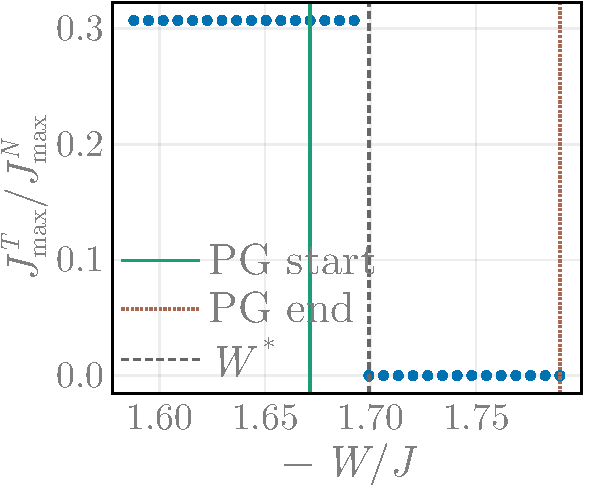
\includegraphics[width=0.45\textwidth]{quadrantMaxKondo-49.pdf}
	\caption{Ratio between the maximum values of the fixed point values of the Kondo couplings for scattering processes between and within the regions \(S^+\) and \(S^-\). The vanishing of the fixed point ratio indicates that the pseudogap regime features a singular low-energy effective theory, where the Fermi surface neighbourhood splits into two disconnected regions with no explicit term in the Hamiltonian connecting them directly.}
	\label{channelDecoupling}
\end{figure}

The decoupling of the \(k-\)space regions \(S^\pm\) is captured by the following simplified low-energy Hamiltonian:
\begin{equation}\begin{aligned}\label{twoChannel}
H_\text{eff} = H(S^+) + H(S^-);~H(S) = \sum_{{\bf q}\in S,\sigma}\varepsilon_{\bf q}c^\dagger_{{\bf q}\sigma}c_{{\bf q}\sigma} + \sum_{{\bf q}_1\in S,{\bf q}_2\in S}\sum_{\alpha,\beta}J^*({\bf q}_1,{\bf q}_2){\bf S}_d\cdot {\bf \sigma}_{\alpha\beta}c^\dagger_{{\bf q}_1\alpha}c_{{\bf q}_2\beta}~,
\end{aligned}\end{equation}
where \(H(S^\pm)\) represents the dynamics of momentum states residing in regions \(S^\pm\). The only source of information transfer between the two regions is the fact that they interact with the same impurity local moment. Eq.\ref{twoChannel} tells us that the low-energy dynamics of the embedded eSIAM close to the Kondo-breakdown transition is governed by an emergent {\bf two-channel Kondo model}, with the conduction bath states in the sets \(S^\pm\) making up the two channels.

\subsection{Momentum-resolved Dynamical Spectral Weight Transfer}
Passage through the PG phase is accompanied by a highly structured transfer of spectral weight across the FS. Strong charge fluctuations develop between the nodal and antinodal regions of the FS in the PG regime of the impurity model (Fig.~\hyperref[chargeCorr]{\ref*{chargeCorr}(a)}), as captured by the correlator:
\begin{equation}
\chi_c({\bf k}_1, {\bf k}2) = \left\langle
c^{\dagger}_{{\bf k}1 \uparrow} c^{\dagger}_{{\bf k}1 \downarrow} c_{{\bf k}2 \downarrow} c_{{\bf k}_2 \uparrow} + \text{h.c.}\right\rangle~.
\end{equation}
These fluctuations dynamically redistribute low-energy spectral weight from the antinodes to higher energies, leading to selective gap formation. Accordingly, the Luttinger surfaces of the PG~\cite{dzyaloshinskii2003some} coincides with the appearance of poles of the lattice model self-energy $\Sigma ({\bf k},\omega=0)$ near the antinodes; these poles approach the nodes on tuning towards the Mott transition (Fig.~\hyperref[chargeCorr]{\ref*{chargeCorr}(b)}). This mirrors the coalescing of finite-frequency poles of the self-energy poles towards zero frequency in the underlying impurity model~(Fig.~\hyperref[chargeCorr]{\ref*{chargeCorr}(c)}). 
\begin{figure*}
    \centering
    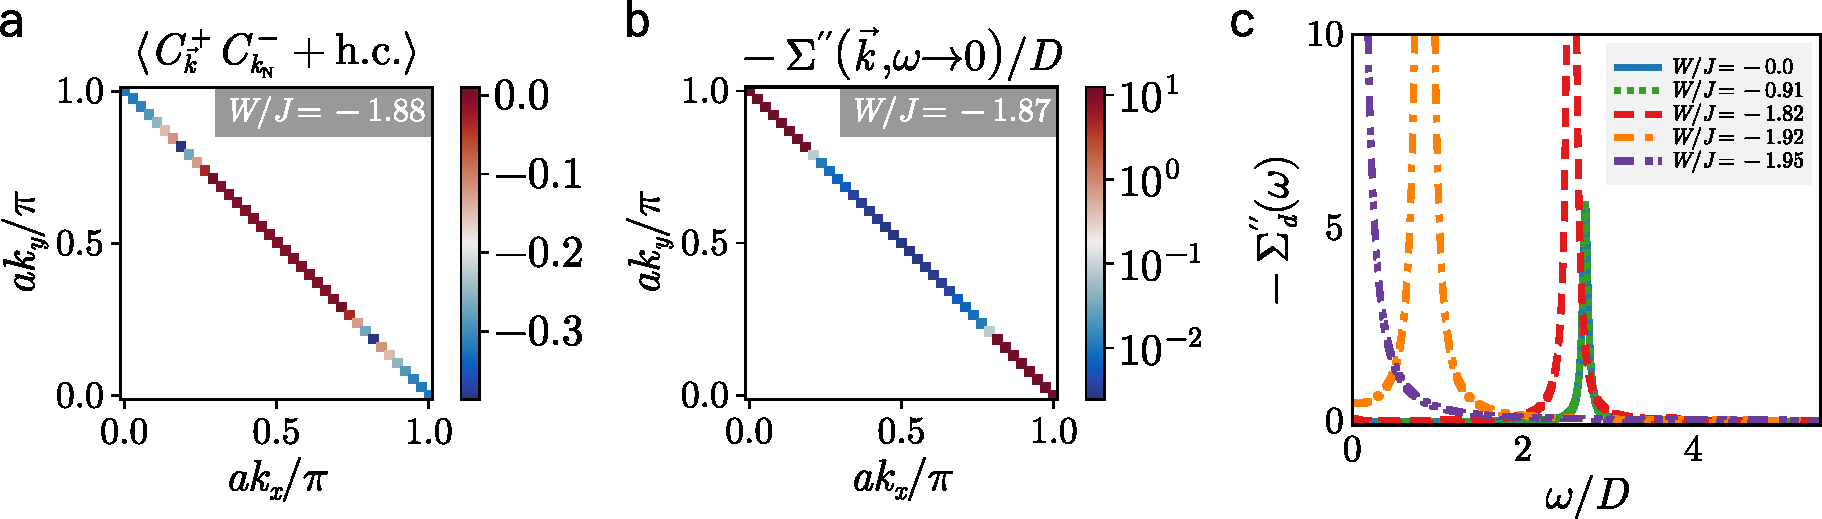
\includegraphics[width=\textwidth]{fig3.pdf}
    \caption{(a) Enhanced charge correlations $\chi_c({\bf k}_1, {\bf k}_2) = \braket{c^\dagger_{{\bf k}_1\uparrow}c^\dagger_{{\bf k}_1\downarrow}c_{{\bf k}_2\downarrow}c_{{\bf k}_2\uparrow} + \text{h.c.}}$ between the nodal and antinodal regions, signalling Kondo breakdown in the pseudogap phase of the impurity model. (b) In turn, the breakdown leads to the gapping of the antinodal regions in the lattice model, seen from the appearance of poles in the imaginary part of the self-energy. (c) The imaginary part of the impurity self-energy $\Sigma^{\prime\prime}(\omega >0)$ possesses a pole at non-zero $\omega$ in the PG that moves towards $\omega=0$ as the Mott transition is approached.}
    \label{chargeCorr}
\end{figure*}




\section{Non-Fermi liquid excitations within the Pseudogap}\label{NFLproperties}
\subsection{Pseudogapped spectral function and singular self-energy}
In the PG regime, the nature of gapless Fermi arcs changes dramatically. We have already argued that the low-energy dynamics of these gapless Fermi arcs are governed by an underlying two-channel Kondo (2CK) impurity model~\cite{Tsvelick_weigmann_mchannel_1985, emery_kivelson}. This is consistent with the rapid fall of the impurity quasiparticle residue $Z_\text{imp}$ (Fig.~\hyperref[channelDecoupling]{\ref*{channelDecoupling}(a)}) from finite values in the FL phase to vanishingly small values just before the onset of the PG. Inset  shows the simultaneous emergence of increasingly uncompensated local magnetic moments upon traversing the PG phase. The accompanying impurity spectral function of the gapless arcs show a pseudogapped behaviour for $\omega\simeq 0$, with a rapid fall in the spectral weight at $\omega=0$ upon traversing the PG~(Fig.~\hyperref[channelDecoupling]{\ref*{channelDecoupling}(c)}). The collapse of the Kondo resonance into a pseudogapped spectral function is accompanied by the redistribution of spectral weight~\cite{dzyaloshinskii2003some} in the impurity spectral function (Fig.~\hyperref[channelDecoupling]{\ref*{channelDecoupling}(b)}) from $\omega\sim 0$ to the Hubbard sidebands at finite frequencies $\omega\simeq \pm 3$ (in units of the bandwidth). 

Concomitant with this is the emergence of a zero-frequency peak in the imaginary part of the self-energy of the NFL in the PG phase(Fig.~\hyperref[selfEnergy]{\ref*{selfEnergy}(a)}),
\begin{equation}
\begin{aligned}
-1/\Sigma^{\prime\prime}(\omega)\sim 1/\Sigma^{\prime\prime}(0) + \omega^{\beta}~.
\end{aligned}
\end{equation}
Remarkably, we find that the exponent $\beta=2$ characterises the NFL for the entire PG phase (see Fig.~\hyperref[selfEnergy]{\ref*{selfEnergy}(b)}), including the critical end-point. This is in stark contrast with the $\Sigma''(\omega)\sim \omega^{2}$ for the FL (Fig.~\hyperref[selfEnergy]{\ref*{selfEnergy}(b)}). A similar analysis reveals the power-law scaling for the low-frequency behaviour of the impurity spectral function in Fig.\ref{ImpSpecFuncFits}. We observe that $A_{d}(\omega)\sim A_d(0) + \omega^{2}$ for the pseudogap phase, while $1/A_{d}(\omega)\sim 1/A_{d}(0) + \omega^{2}$
for the Fermi liquid (inset of Fig.~\ref{ImpSpecFuncFits}).
\subsection{Finite-Frequency Scattering Rate and Optical Response Through the Pseudogap}
All $\Sigma''(\omega)$ for the NFL are observed to lie above the Mott-Ioffe-Regel (MIR) bound~\cite{GunnarssonRMP2003,Hussey2004} (dashed blue line in Fig.~\hyperref[selfEnergy]{\ref*{selfEnergy}(a)}), while those for the FL lie below. The MIR bound is the maximum expected scattering rate in metals when the mean free path approaches the lattice spacing: 
\begin{equation}
\begin{aligned}
-2\Sigma^{\prime\prime}_\text{MIR} = 1/\tau_\text{MIR}~, ~\tau_\text{MIR} = l_\text{min}/v_{F}~,
\end{aligned}
\end{equation}
where $l_\text{min}$ is the minimum mean free path in metals (equal to one lattice spacing) and $\tau_\text{MIR}$ is the associated lifetime of quasiparticles close to the FS (with Fermi velocity $v_F$). 
% The optical conductivity $\sigma (\omega)$ of the NFL thus undergoes a suppression as $\omega \to 0$, together with a shift of the Drude peak to finite $\omega$~\cite{Hussey2004,pustogow2021}. 
The height of the zero-frequency peak rises by almost 4 orders of magnitude from the start of the PG till its end at the Mott transition point (Fig.~\hyperref[selfEnergy]{\ref*{selfEnergy}(c)}); the dramatic growth of the peak height very near the Mott critical point coincides with the coalescing of the finite-frequency poles of the self-energy into a single pole at zero-frequency, signalling the singular nodal NFL present at the Mott quantum critical point.

To further probe the breakdown of coherent transport in the pseudogap (PG) regime, we examine the product of the impurity spectral function $A(\omega)$ and the scattering lifetime $\tau(\omega)$, which approximates the optical conductivity $\sigma(\omega)$ via a Drude-type relation. As shown in the main panel of Fig.~\ref{optical}, this quantity exhibits a sharp Drude peak at $\omega = 0$ in the Fermi liquid (FL) regime (blue), consistent with long-lived quasiparticles. In stark contrast, the PG regime (green, red, orange) shows a pronounced suppression of low-frequency conductivity and the emergence of a finite-frequency peak centered near $\omega/D \sim 0.3{-}0.4$ (where $D$ is the kinetic energy bandwidth).



\begin{figure*}[!ht]
    \centering
    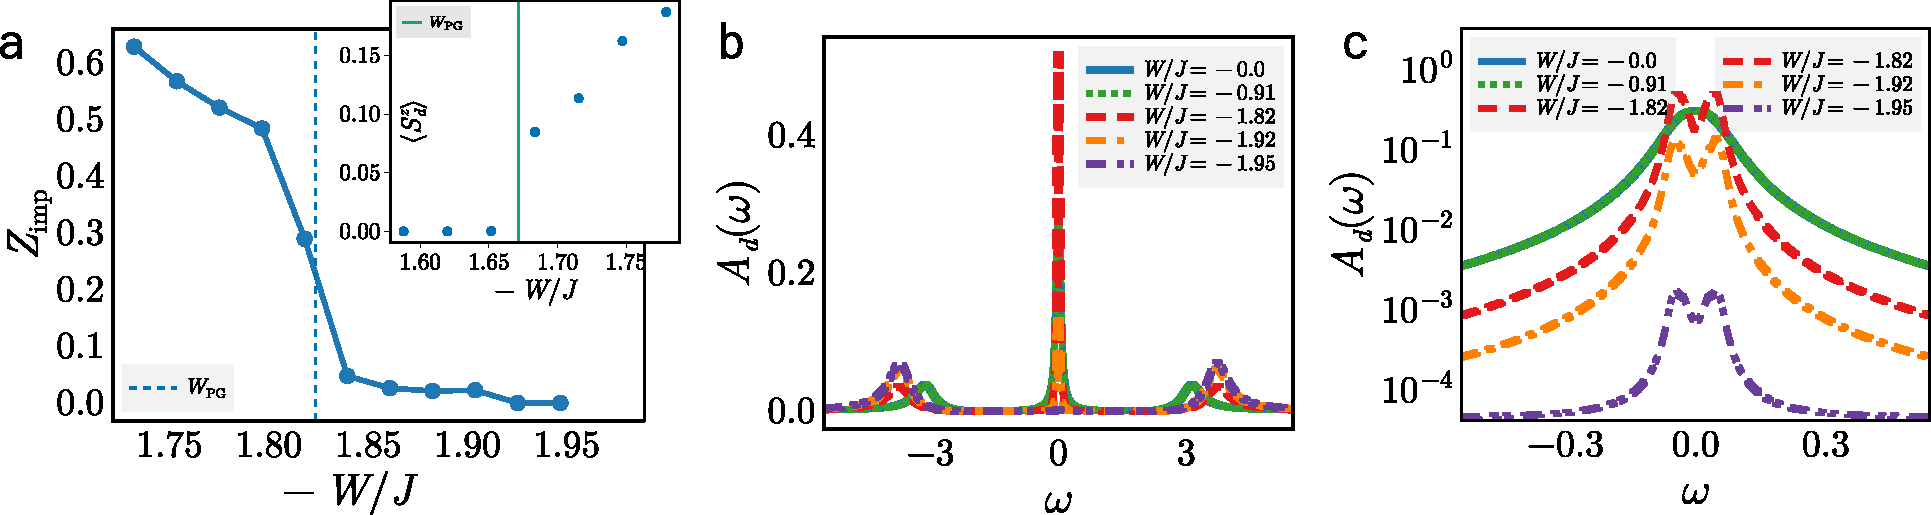
\includegraphics[width=\textwidth]{fig4.pdf}
    \caption{(a) Suppression of quasiparticle residue ($Z_\text{imp}$) as the impurity model is tuned towards the Mott transition. An initial drastic fall in $Z_\text{imp}$ is observed for $W/J \lesssim (W/J)_\text{PG}$ from $0.3$ to around $0.05$, signalling the destruction of the FL with unravelling of Kondo screening. A steady decrease in $Z_{imp}$ is observed in passage through the PG, and is vanishingly small close to the Mott transition due to a divergent self-energy. Inset shows the growth of unscreened impurity magnetic moment in the pseudogap phase, signalling the breakdown of Kondo screening. (b) Impurity Spectral function in the FL and PG phases. The evolution of the central peak from Kondo resonance to pseudogap is accompanied by dynamical spectral weight transfer to the Hubbard side bands at finite frequencies $\omega\simeq \pm 3$ (in units of the bandwidth). (c) Zoom-in of the central (Kondo) resonance of the impurity spectral function. While undisturbed in the Fermi liquid phase, it splits into a pseudogap in the PG phase, with its height diminishing rapidly as the Mott transition is approached.
    }
    \label{channelDecoupling}
\end{figure*}
Strikingly, this peak shifts very little across the PG regime (see inset), despite a deepening spectral gap and diverging self-energy. Its position lies well below the Mott gap ($\sim 2.5D$), suggesting that it represents an emergent mid-infrared (MIR) excitation intrinsic to the Mott metal characterising the PG. This feature closely mirrors the experimentally observed MIR peak in high-T$_\text{c}$ cuprates~\cite{Herr1987,Orenstein1987,Uchida1991}, which has been variously attributed to excitations of electrons bound to vacancies~\cite{Thomas1992Optical}, or the dressing of holes by spin excitations~\cite{Dagotto1994RMP}. Here, its robust energy scale and insensitivity to increasing incoherence imply a universality persisting through the PG, likely rooted in short-range entanglement between deconfined doublons and holons excitations of the Mott metal. This is further evidence that the PG metal is not simply a degraded Fermi liquid, but a distinct phase whose optical response is driven by emergent degrees of freedom.



\subsection{Non-local correlations in the pseudogap}
In Fig.~\hyperref[longranged]{\ref*{longranged}(a)} and \hyperref[longranged]{\ref*{longranged}(b)}, the spin-flip correlations and mutual information between the impurity spin and conduction bath sites respectively are observed to undergo a crossover within the PG, from a short-ranged behaviour at its onset, to a long-ranged behaviour as the Mott transition approaches. The entanglement is also observed to be multipartite in nature: in Fig.~\hyperref[longranged]{\ref*{longranged}(c)}, the quantum Fisher information (QFI)~\cite{Hauke2016} computed for the ground state wavefunction using an operator corresponding to the sum of local spin-flip exchange processes shows a jump at the onset of the PG. Further, the FL is observed to possess bi-partite entanglement while the NFL of the PG phase displays pentapartite entanglement~\cite{balut2025,mazza2024}.

These striking results imply that the Mott transition observed by us lies beyond the local quantum criticality scenario~\cite{Si2001}. Instead,  we observe the PG phase to be a novel state of strongly interacting quantum matter emergent from the breakdown of local Kondo screening. This state is described by a quantum critical Fermi surface~\cite{senthil2008CriticalFermiSurface} with NFL Fermi arcs that display increasingly critical behaviour, i.e., dynamics described by non-local quantum fluctuations, and excitations that become truly long-ranged close to the transition. It is tempting to conjecture that the long-range entangled critical state captured in Fig.~\hyperref[longranged]{\ref*{longranged}(b)} reflects the existence of a highly efficient scrambler~\cite{sekino2008,hayden2007,bentsen2019}, i.e., a state in which entanglement spreads among its constituents at the fastest rate permissible by quantum mechanics.  

\section{Exactly solvable nodal Non-Fermi liquid at Mott Criticality}\label{exactsolforMottCrit}
Very close to the transition, the excitations of the nodal NFL correspond to those of a Hatsugai-Kohmoto model~\cite{Baskaran1991,Hatsugai1992}. This insight is obtained from a perturbation-theoretic treatment of the RG fixed point Hamiltonian of the impurity model for $W/J\lesssim (W/J)_{\text{PG}}$, by considering the effects of a small fixed point Kondo scattering probability \(J^*\) in the backdrop of a larger bath interaction parameter \(|W|\). This yields the HK model~\cite{Baskaran1991,Hatsugai1992} as the singular part of the effective Hamiltonian arising from forward scattering processes.


As the bath interaction \(W\) is tuned through the L-PG phase, the nodal region is the last to decouple from the impurity. This allows us to write down a simpler Kondo model near the transition, where only the nodal region is hybridising with the impurity spin through Kondo interactions. This is done by retaining only those scattering processes \({\bf k}_1 \to {\bf k}_2\) that originate from and end at \(k-\)points within a small neighborhood of width \(|{\bf q}|\) around the four nodal points: \({\bf k}_1, {\bf k}_2 \in {\bf N} + {\bf q}, |{\bf q}| \ll \pi\), where \({\bf N}\) can be any one of the four nodal points \({\bf N}_{1} = \left(\pi/2, \pi/2\right), {\bf N}_{2} = \left(-\pi/2, \pi/2\right)\) and \({\bf N}_1 + {\bf Q}_1\) and \({\bf N}_{2} + {\bf Q}_2\), where \({\bf Q}_1 = \left(-\pi,-\pi \right)\) and \({\bf Q}_2 = \left( \pi, -\pi \right) \) are the two nesting vectors. We assume that the window of \({\bf q}\) is small enough so that the fixed point Kondo coupling values \(J^*({\bf q}_1, {\bf q}_2)\) for the scattering processes involving \({\bf q}_1\) and \({\bf q}_2\) can be replaced by an average value \(J^*\).

With these considerations, the simplified low-energy model near the transition describing the Kondo scattering processes can be written as
\begin{equation}\begin{aligned}
	\tilde H_\text{imp-cbath} = J^*\frac{1}{2}\sum_{l=1,2}\sum_{{\bf q}_1, {\bf q}_2}\sum_{\alpha,\beta}{\bf S}_d\cdot{\boldsymbol \sigma}_{\alpha\beta}\left(c^\dagger_{{\bf N}_l + {\bf q}_1,\alpha}c_{{\bf N}_l + {\bf q}_2,\beta} + c^\dagger_{{\bf N}_l + {\bf Q}_l + {\bf q}_1,\alpha}c_{{\bf N}_l + {\bf Q}_l + {\bf q}_2,\beta}  - c^\dagger_{{\bf N}_l + {\bf Q}_l + {\bf q}_1,\alpha}c_{{\bf N}_l + {\bf q}_2,\beta} \right.\\
    \left.- c^\dagger_{{\bf N}_l + {\bf q}_1,\alpha}c_{{\bf N}_l + {\bf Q}_l + {\bf q}_2,\beta}\right)~.
\end{aligned}\end{equation}
The label \(l\) can take values 1 or 2, allowing us to consider both the decoupled channels in the PG (associated with \({\bf N}_1\) and \({\bf N}_2\)). It also labels the nesting vectors \({\bf Q}_l\) associated with the two sets. \(\alpha\) and \(\beta\) indicate spin indices, and \({\bf q}_1\) and \({\bf q}_2\) represent incoming and outgoing momenta in the scattering processes.

Because of the decoupling of the channel \(l=1\) and \(l=2\), we consider only the \(l=1\) channel for the rest of the calculations in this section. In order to simplify the Hamiltonian, we define new fermionic operators
\begin{equation}\begin{aligned}
	\psi_{{\bf q}, \sigma} = \frac{1}{\sqrt 2}\left(c_{{\bf N}_1 + {\bf q},\sigma} + c_{{\bf N}_1 + {\bf Q}_1 - {\bf q}, \sigma}\right)~, ~\phi_{{\bf q}, \sigma} = \frac{1}{\sqrt 2}\left(c_{{\bf N}_1 + {\bf q},\sigma} - c_{{\bf N}_1 + {\bf Q}_1 - {\bf q}, \sigma}\right)~,
\end{aligned}\end{equation}
The operator satisfy fermionic anticommutation relations. For convenience, we define new number operators for the sum and relative degrees of freedom:
\begin{equation}\begin{aligned}
	s_{{\bf q},\sigma} = {\psi}^\dagger_{{\bf q}} {\psi}_{{\bf q}},~ r_{{\bf q},\sigma} = {\phi}^\dagger_{{\bf q}} {\phi}_{{\bf q}}~.
\end{aligned}\end{equation}
We then have the following useful relation between the corresponding number operators \(n = c^\dagger c\):
\begin{equation}\begin{aligned}\label{numberOperatorRelation}
	n_{{\bf N}_1 + {\bf q},\sigma} + n_{{\bf N}_1 + {\bf Q}_1 - {\bf q}, \sigma} = s_{{\bf q}, \sigma} + r_{{\bf q},\sigma}~.
\end{aligned}\end{equation}

In terms of these new degrees of freedom, the auxiliary model Hamiltonian takes the form
\begin{equation}\begin{aligned}
	\tilde H = -\frac{1}{2}W\sum_{{\bf q},\sigma}r_{{\bf q},\sigma} + W\sum_{{\bf q}_1,{\bf q}_2}r_{{\bf q}_1,\uparrow} r_{{\bf q}_2,\downarrow} + \sum_{{\bf q}_1, {\bf q}_2,\alpha,\beta}J^*{\bf S}_d\cdot{\boldsymbol\sigma}_{\alpha\beta} {\phi}^\dagger_{{\bf q}_1\alpha} \phi_{{\bf q}_2\beta} + \sum_{{\bf q},\sigma}\varepsilon_{{\bf N}_1 + {\bf q}}\left({\psi}^\dagger_{{\bf q},\sigma} {\phi}_{{\bf q},\sigma} + {\phi}^\dagger_{{\bf q},\sigma} \psi_{{\bf q},\sigma}\right),
\end{aligned}\end{equation}
where we have considered a simplified form of the bath interaction (for the channel \(l=1\)), taking into account the density-density correlations in \(k-\)space. 

For bath interaction strength close to the critical value (\(W \lesssim W_c\)), the fixed point coupling value \(J^*\) is much smaller than \(W\). In order to obtain the gapless excitations of the system arising from the presence of the impurity site, we integrate out the impurity dynamics via a Schrieffer-Wolff transformation. The perturbation term \(\mathcal{V}\) then consists of Hamiltonian terms that modify the impurity configuration,
\begin{equation}\begin{aligned}
	\mathcal{V} = \sum_{{\bf q},\sigma}\varepsilon_{{\bf N}_1 + {\bf q}}\left({\psi}^\dagger_{{\bf q},\sigma} {\phi}_{{\bf q},\sigma} + {\phi}^\dagger_{{\bf q},\sigma} \psi_{{\bf q},\sigma}\right) + \sum_{{\bf q}_1, {\bf q}_2}J^*{S}_d^+{\phi}^\dagger_{{\bf q}_1 \downarrow} \phi_{{\bf q}_2 \uparrow} + \text{h.c.}~,
\end{aligned}\end{equation}
while the ``non-interacting" Hamiltonian is
\begin{equation}\begin{aligned}
	H_D &= -\frac{1}{2}W\sum_{{\bf q},\sigma}r_{{\bf q},\sigma} + W\sum_{{\bf q}_1,{\bf q}_2}r_{{\bf q}_1,\uparrow} r_{{\bf q}_2,\downarrow}~.
\end{aligned}\end{equation}
For the present Hamiltonian, the low-energy state is the one that minimises the bath interaction term \(\tilde H_\text{cbath-int}\). High-energy states are obtained by applying, on the state \(\ket{L}\), the excitation operator \(\phi^\dagger_{{\bf q}_1,\sigma}\phi_{{\bf q}_2,\bar\sigma}\) or its hermitian conjugate.

The complete second-order renormalised Hamiltonian is
\begin{equation}\begin{aligned}
    \Delta \tilde H =& \sum_{{\bf q}, \sigma}\epsilon_{\bf q} r_{{\bf q},\sigma} + \mathcal{U}\sum_{{\bf q}, \sigma}r_{{\bf q} \sigma}r_{{\bf q} \bar\sigma} + \mathcal{U}\sum_{{\bf q}_1 \neq {\bf q}_2, \sigma}\left[r_{{\bf q}_1 \sigma}r_{{\bf q}_2 \bar\sigma} + \phi^\dagger_{{\bf q}_1,\bar\sigma}\phi^\dagger_{{\bf q}_1,\sigma}\phi_{{\bf q}_2, \sigma}\phi_{{\bf q}_2, \bar\sigma}\right]~.
\end{aligned}\end{equation}
where $\epsilon_{\bf q} = \text{sign}\left(\varepsilon_{{\bf N}_1 + {\bf q}}\right)\frac{\varepsilon_{{\bf N}_1 + {\bf q}}^2}{-W}$ and $\mathcal{U} = \frac{{J^*}^2}{4W}$.

\begin{figure*}
    \centering
    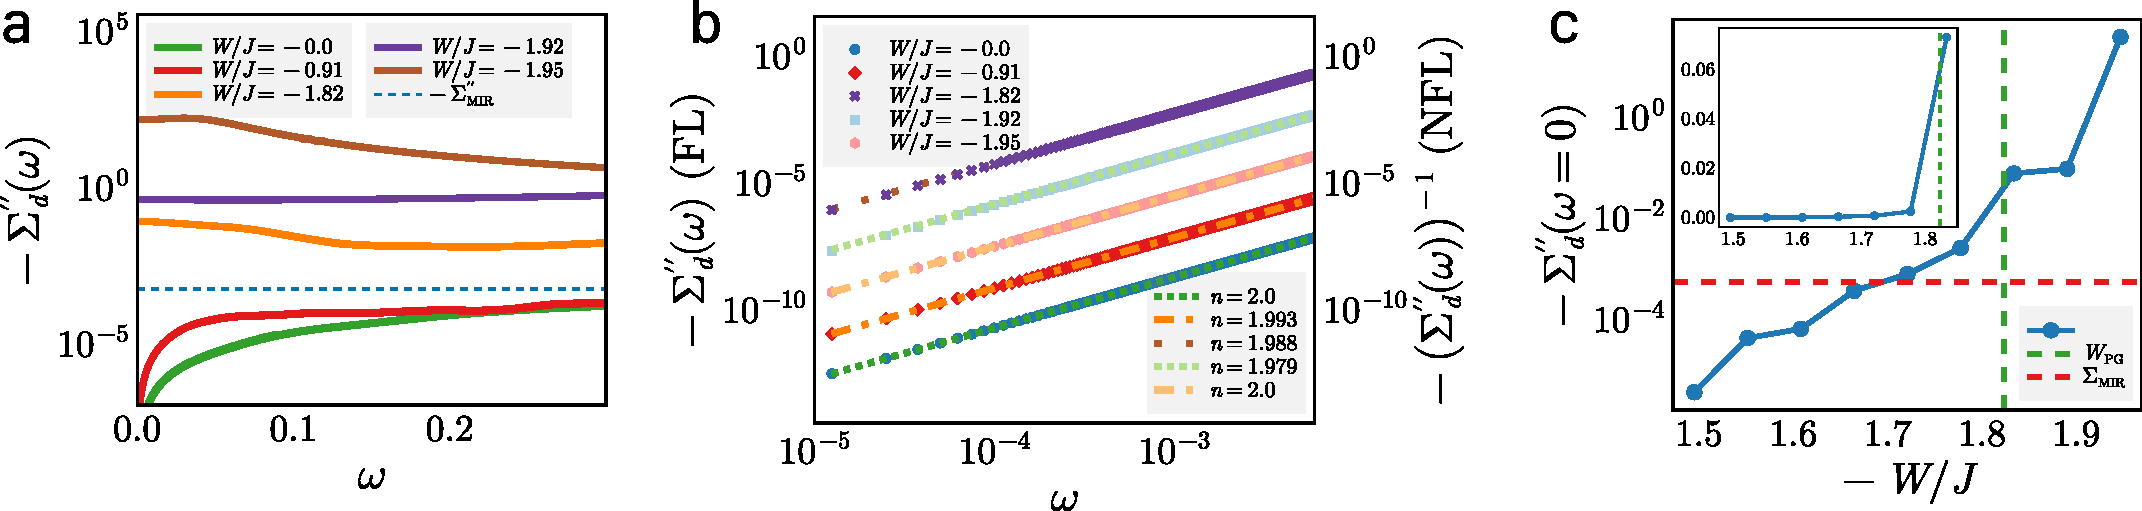
\includegraphics[width=\textwidth]{fig5.pdf}
    \caption{(a) Imaginary part of impurity self-energy $\Sigma^{\prime\prime}(\omega)$ as a function of frequency $\omega$ for Fermi liquid (FL, $|W/J| < 1.79$) and pseudogapped phases (NFL, $|W/J| \geq 1.79$). $\Sigma''(\omega)$ falls to zero as $\omega\to 0$ for the FL, while it attains a peak in the pseudogap. All $\Sigma''(\omega)$ for the NFL are observed to lie above the Mott-Ioffe-Regel (MIR) bound (dashed blue line), while those for the FL lie below. (b) Scaling of $\Sigma^{\prime\prime}(\omega)$ with frequency for Fermi liquid and pseudogapped phases. The FL self-energy fits to $\Sigma^{\prime\prime} \sim \omega^{\alpha}$ with $\alpha\approx 2$, vanishing as $\omega\to 0$, while the NFL self-energy grows as $\Sigma^{\prime\prime} \approx a - \omega^{\beta}$ for small $\omega$, with $\beta\approx 2$. Remarkably, the NFL exponent remains mostly unchanged through the entirety of the PG phase. (c) Variation of the zero-frequency imaginary self-energy $-\Sigma''(\omega=0)$ with $\omega$ in the FL and pseudogap phases (entry into the PG is marked by the vertical dashed line). The inset shows the same but in linear scale, in order to display the dramatic rise (by almost 30 times) on entering the PG.}
    \label{selfEnergy}
\end{figure*}

\begin{figure}[!hbtp]
    \centering
    \hspace*{-1cm}
    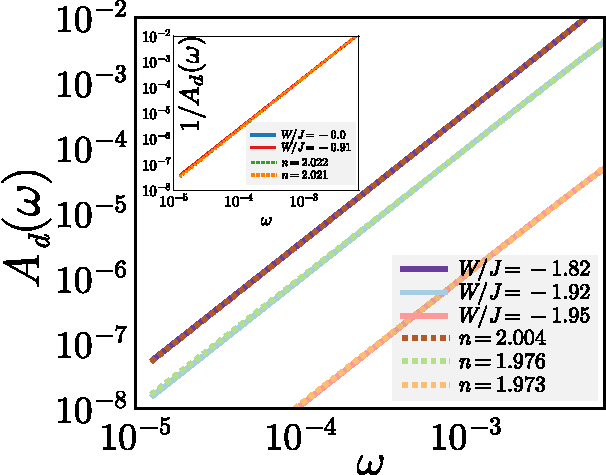
\includegraphics[width=0.9\linewidth]{Ad_fit.pdf}
    \caption{Impurity spectral function $A_d(\omega)$ in the local Fermi liquid (inset) and pseudogap (main). The PG spectral function is fit to a power law (with the $\omega=0$ contribution subtracted, see Fig.~\hyperref[selfEnergy]{\ref*{selfEnergy}(c)} for the full spectral function). The exponent of the power law comes out to be $n\approx 2$ throughout the PG. The local FL spectral function (inset) is fit to a lorentzian (by fitting the inverse to a power law).
    }
    \label{ImpSpecFuncFits}
\end{figure}

\begin{figure}[!ht]
	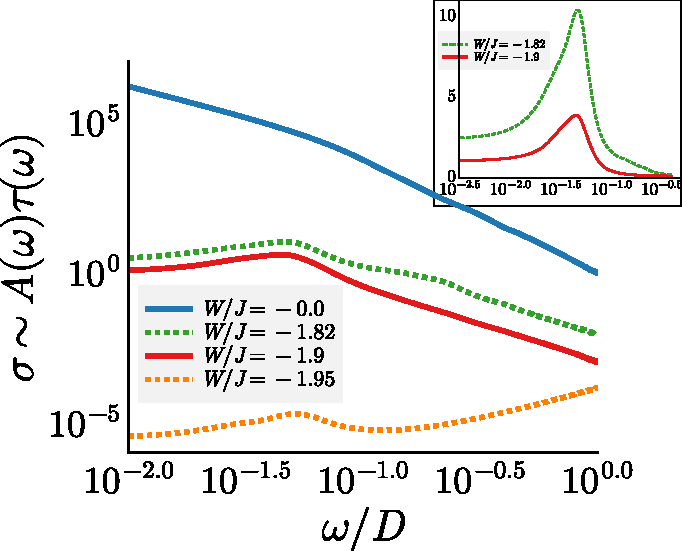
\includegraphics[width=0.48\textwidth]{sigma_in.pdf}
	\caption{Optical conductivity $\sigma(\omega)$ for excitations of the impurity model, approximated through the product of the carrier density (taken from the density of states $A(\omega)$) and the lifetime $\tau(\omega)$ (obtained from the inverse scattering rate $-1/\Sigma^{\prime\prime}(\omega)$, where $\Sigma^{\prime\prime}$ is the imaginary part of the self-energy). The Fermi liquid (blue) shows a sharp Drude peak at $\omega=0$ due to the presence of long-lived quasiparticles. The PG (green, red, orange) shows a shifted Drude peak at a non-zero frequency which is reminiscent of the mid-infrared (MIR) peak seen experimentally in the cuprates~\cite{Herr1987,Orenstein1987,Uchida1991}. Inset shows the robustness of the position of the MIR peak through the PG, indicating it as a universal feature of the Mott metal.}
	\label{optical}
\end{figure}
 
The ${\bf q}_1={\bf q}_2$ component of the Hamiltonian shows the emergence of the exactly solvable Hatsugai-Kohmoto model~\cite{Baskaran1991,Hatsugai1992} 
at the critical point. The correlation term $\mathcal{U}\sum_{{\bf q}, \sigma}r_{{\bf q} \sigma}r_{{\bf q} \bar\sigma}$ leads to a transfer of spectral weight across the Fermi surface and separates the available states into three classes:
\begin{equation}\begin{aligned}
\braket{n_{\bf q}} = \begin{cases}
    2, \quad \epsilon_{\bf q} < -|\mathcal{U}/2|~,\\
    1, \quad |\mathcal{U}/2| > \epsilon_{\bf q} > -|\mathcal{U}/2|~,\\
    0, \quad |\mathcal{U}/2| < \epsilon_{\bf q}~.
\end{cases}
\end{aligned}\end{equation}
In constrast to a Fermi liquid, there is a highly degenerate single-occupied region in the middle, and this gives rise to non-Fermi liquid excitations.

We now discuss the effects of the ${\bf q}_1 \neq {\bf q}_2$ component. The first term partially lifts the degeneracy of the central singly-occupied region and allows only zero magnetisation configurations. The second term creates gapped excitations involving the regions of zero and double occupancy; these represent subdominant pairing fluctuations of the nodal non-Fermi liquid. {\color{blue} We recall that similar fluctuations across the Fermi surface were observed in our calculations of charge correlations in Fig.~\ref{chargeCorr} (a), and are consistent with pairing fluctuations observed from quantum Monte Carlo simulations and found to give rise to quantum-critical behavior and PG physics~\cite{Jiang2022}.}

Consequently, the resulting NFL metal of the lattice model involves long-lived excitations of multiple \({\bf k}\)-states, and manifest in the form of a divergent one-particle self-energy at the non-interacting FS~\cite{Phillips2020}:
$\Sigma_{{\bf q}}(\omega) = -\mathcal{U}^2/4(\omega - \epsilon_{\bf q})$~, such that $\Sigma_{\epsilon_{\bf q}=0}(\omega \to 0)  \to \infty$. This zero-frequency self-energy pole presages the transition into a Mott insulating phase, where it marks a hard gap in the spectral function for charge excitations. This is consistent with our findings for the lattice (Fig.~\hyperref[chargeCorr]{\ref*{chargeCorr}(c)}) and impurity self-energies~(Fig.~\hyperref[selfEnergy]{\ref*{selfEnergy}(c)}). The nodal Mott metal thus comprises of a Greens function zero at the Fermi energy together with an anistropic massless Dirac dispersion, leading to a non-zero Chern number~\cite{vafekvishwanath2014,morimoto2016,calderon2025}. This topological index survives into the Mott insulator.

For small but non-zero values of \(\omega - \epsilon_{\bf k}\), we obtain a quasiparticle residue that vanishes with $\omega$, \(Z_\text{imp} \sim \omega^2/\mathcal{U}^2 \). The scattering rate of this singular NFL possesses a sharp peak at the FS (\(\omega=\epsilon_{\bf k_{\mathrm{F}}}\)): 
\begin{equation}\begin{aligned}
\Gamma \sim \mathcal{U}^2\delta(\omega - \epsilon_{\bf k})~,
\end{aligned}\end{equation}
consistent with the sharply peaked Lorentzian $\Sigma''_{{\bf k}}(\omega)\sim \omega^{-2}$ captured in Fig.~\hyperref[selfEnergy]{\ref*{selfEnergy}(a)}. This quantum critical NFL metal is an example of a strongly coupled scale-invariant form of quantum matter. The exact solution for eq.\eqref{HKModel} reveals the presence of low-energy excitations comprised of holons and doublons~\cite{Hatsugai1992}. These features point to the nodal NFL as a long-ranged and multipartite entangled, strongly interacting scale-invariant state of quantum matter 
~\cite{Georgi2007PRL,Georgi2007,Phillips2013Unparticles,PhillipsLectures2014} that are completely disconnected from the quasiparticles of the FL. Following the arguments laid out in~\cite{phillips2022}, at finite temperatures, such a scale-invariant highly entangled non-Fermi liquid is likely associated with Planckian dissipation (i.e., $\Sigma'' (T)\sim k_{B}T$) and a resistivity that varies linearly with temperature ($\rho\sim T$)~\cite{zaanen2019,legros2019,hartnoll2022}. This sits well with the possibility that this state is also a highly efficient scrambler~\cite{sekino2008,hayden2007,bentsen2019}. Additionally, as mentioned above, we observe that the nodal metal possesses pairing fluctuations that can become dominant upon doping~\cite{Phillips2020}.

\begin{figure*}
    \centering
    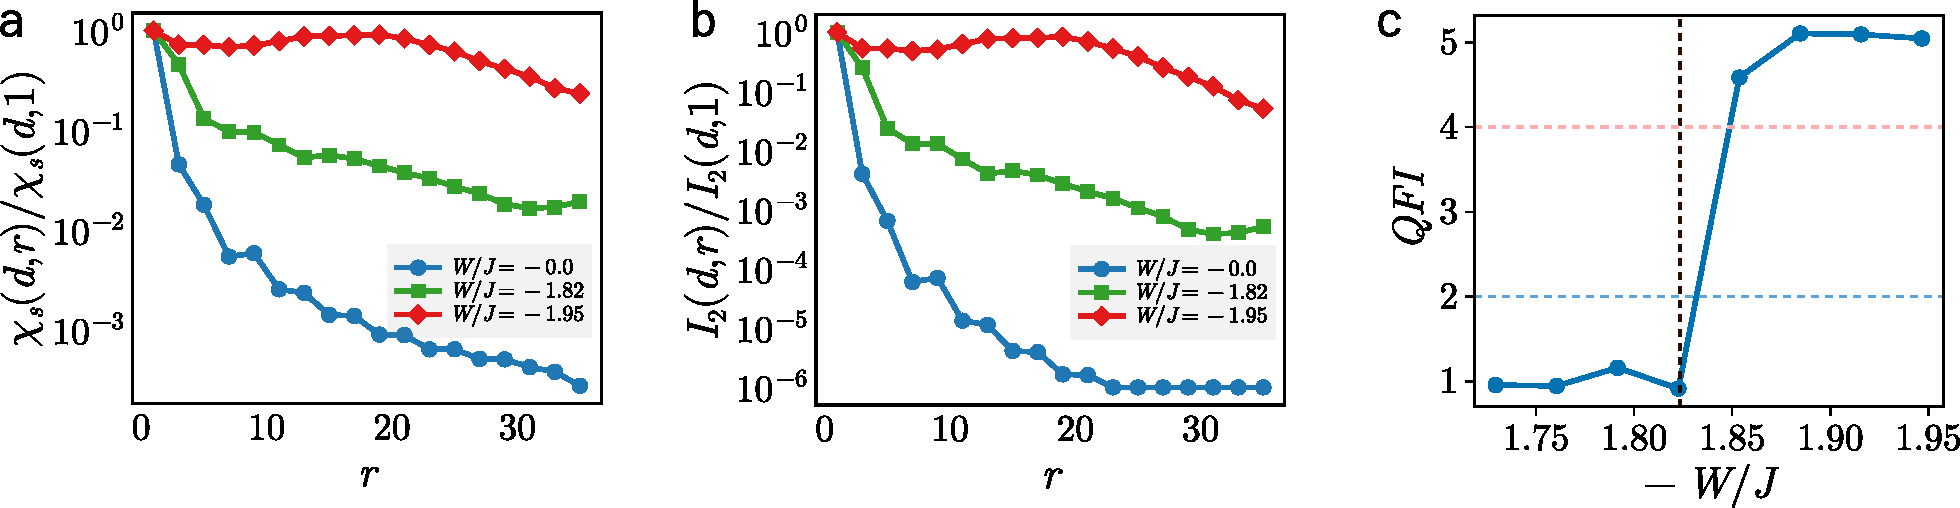
\includegraphics[width=\textwidth]{fig6.pdf}
    \caption{(a) Spin correlation $\braket{{\bf S}_d \cdot {\bf S}_r}$  and (b) mutual information $I_{2}(d,r)$  between the impurity spin and conduction bath local spin density as a function of the distance {\bf r} between them, normalised against the value at $r=1$. Both decay very quickly in the FL phase (blue), but show long-ranged behaviour in the NFL phase (green and red), extending to the edges of the system at the critical point (red). (c) Evolution of the Quantum Fisher Information $F_Q$ for a nearest-neighbour spin-flip operator $\mathcal{O} = \sum_{i \in \text{odd}}(S_i^+S_{i+1}^- + \text{h.c.})$ through the first Lifshitz transition and the pseudogap. The vertical dashed line marks the onset of the PG. To the left of it, the QFI in the Fermi liquid phase shows at most bipartite entanglement ($F_Q < 2$ (below blue dashed line)), while the PG shows the presence of multipartite entanglement upto 5 parties ($F_Q > 4$ (red dashed line)).}
    \label{longranged}
\end{figure*}

\section{Heisenberg Model as a low-energy description of the tiled Mott insulator}\label{heisenbergDerivation}
For simplicity, we consider two impurity sites labelled \(1\) and \(2\) associated with two nearest-neighbour auxiliary models. The ground state subspace is four-fold degenerate:
\begin{equation}\begin{aligned}
	\ket{\Psi_L} = \left\{\ket{\sigma_1,\sigma_2}\right\}~,\quad \sigma_i = \pm 1~,
\end{aligned}\end{equation}
where \(\sigma_i\) is the spin state of site \(i\). This ground state is derived from the following "zeroth order" Hamiltonian that emerges in the local moment phase of the auxiliary models when all scattering processes between the impurity and conduction bath are RG-irrelevant:
\begin{equation}\begin{aligned}
	H_0 = -\frac{U}{2}\sum_{i=1,2}\left(n_{i \uparrow} - n_{i \downarrow}\right)^2~;
\end{aligned}\end{equation}
the local correlation on the impurity site becomes the largest scale in the problem in this phase and pushes the \(\ket{n_i=2}\) and \(\ket{n_i=0}\) states to high energies. This then defines the high-energy subspace for our calculation:
\begin{equation}\begin{aligned}
	\ket{\Psi_H} = \ket{C_1,C_2}~,
\end{aligned}\end{equation}
where \(C_i\) can take values 0 or 2, indicating that the state \(i\) is either empty or full, respectively. Both the double and hole states exist at a charge gap of the order of \(U/2\) above the low-energy singly-occupied subspace defined by the states \(\ket{\Psi_L}\).

In order to allow virtual fluctuations that can lift the large ground state degeneracy and lower the energy, we consider (perturbatively) the effects of an irrelevant single-particle hybridisation that connects the nearest-neighbour sites. This perturbation Hamiltonian is therefore of the form
\begin{equation}\begin{aligned}
	H_t = \sum_\omega V(\omega) \mathcal{P}(\omega)~\sum_\sigma\left(c^\dagger_{1\sigma}c_{2\sigma} + \text{h.c.}\right) ~,
\end{aligned}\end{equation}
where \(V(\omega)\) only acts on states at the energy scale \(\omega\); the renormalisation of \(V\) is encoded in the fact that \(V(\omega)\) is largest for the excited states and vanishes at low-energies: \(V(\omega \to 0) = 0\).

In order to obtain a low-energy effective Hamiltonian for the impurity sites arising from this hybridisation, we integrate out \(H_t\) via a Schrieffer-Wolff transformation. This leads to the following second-order Hamiltonian:
\begin{equation}\begin{aligned}
	H_\text{eff} = \mathcal{P}_L H_t G\mathcal H_t \mathcal{P}_L~.
\end{aligned}\end{equation}
The operator \(\mathcal{P}_L\) projects onto the low-energy subspace \(\ket{\Psi_L}\) - this ensures that we remain in the low-energy subspace at the beginning and at the end of the total process. The Greens function \(G = (E_L - H_0)^{-1}\) incorporates the excitation energy to go from the low-energy subspace \(\ket{\Psi}_L\) (of energy \(E_L\)) to the excited subspace \(\ket{\Psi}_H\) of energy \(E_L + U/2\). Substituting the form of the perturbation Hamiltonian and the excitation energy into the above expression gives
\begin{equation}\begin{aligned}\label{effHam1}
	H_\text{eff} = \frac{V_H^2}{-U/2}\sum_{\sigma,\sigma^\prime} \left[c^\dagger_{1\sigma}c_{2\sigma}c^\dagger_{2\sigma^\prime}c_{1\sigma^\prime} + c^\dagger_{2\sigma}c_{1\sigma}c^\dagger_{1\sigma^\prime}c_{2\sigma^\prime}\right] ~.
\end{aligned}\end{equation}
where \(V_H \equiv V(\omega \to U/2)\) is the impurity-bath hybridisation at energy scales of the order of the Mott gap, in the sense of an RG flow. Terms with consecutive creation or annihilation operators on the same site are prohibited because each site is singly-occupied in the ground state. It is now easy to cast this Hamiltonian into a more recognizable form. For \(\sigma^\prime=\sigma\), we get
\begin{equation}\begin{aligned}
	\sum_{\sigma}\delta_{\sigma,\sigma^\prime}c^\dagger_{1\sigma}c_{2\sigma}c^\dagger_{2\sigma^\prime}c_{1\sigma^\prime} = \sum_\sigma \left(n_{1\sigma} - n_{1\sigma}n_{2\sigma}\right) ~,
\end{aligned}\end{equation}
while \(\sigma=-\sigma^\prime=\pm 1\) gives 
\begin{equation}\begin{aligned}
	\sum_{\sigma}\delta_{\sigma,-\sigma^\prime}c^\dagger_{1\sigma}c_{2\sigma}c^\dagger_{2\sigma^\prime}c_{1\sigma^\prime} = -\left(S_1^+ S_2^- + \text{h.c.}\right)~.
\end{aligned}\end{equation}
For the latter expression, we introduced the local spin-flip operators \(S_i^\pm\). The expression above it can also be cast into spin variables, using the equations
\begin{equation}\begin{aligned}
	\frac{1}{2}\sum_{\sigma}n_{i\sigma} = \frac{1}{2},\\
    \frac{1}{2}\sum_{\sigma}\sigma n_{i\sigma} = S_i^z,
\end{aligned}\end{equation}
where the first equation is simply the condition of half-filling at each site, and the second equation is the definition of the local spin operator in \(z-\)direction. Adding and subtracting the equations gives \(n_{i\sigma} = \frac{1}{2} + \sigma S_i^z\)~.

Substituting everything back into eq.~\ref{effHam1} and dropping constant terms gives
\begin{equation}\begin{aligned}
	H_\text{eff} = 2\frac{V_H^2}{U/2}\left(2S_1^z S_2^z + S_1^+S_2^- + S_1^-S_2^+\right) = J_\text{eff} {\bf S}_1\cdot{\bf S}_2~,
\end{aligned}\end{equation}
where the effective antiferromagnetic Heisenberg coupling is \(J_\text{eff} = \frac{8V_H^2}{U}\).
\section{Pseudogap as a strongly coupled phase of quantum matter}\label{pseudogapasnovelphase}
We now unveil an organising principle that leads to the remarkable properties observed above for the strongly interacting NFL of the PG phase. The existence of a sharp connected FS at $T=0$ can be understood as the existence of a topologically protected manifold of gapless chiral excitations in ${\bf k}$-space at the FS~\cite{Heath_2020}. The FS is characterised by a topological index corresponding to an anomaly in the quantum many-body theory for electrons, and can be understood as a generalised symmetry of such a system~\cite{lanave2025,McGreevy2023}. A theorem by Luttinger and Ward~\cite{luttinger1960ground} shows that a count of the physical charge (known as Luttinger's volume) is identical to the topological index (a so-called homotopy charge known as Luttinger's count) even in the presence of electronic interactions that do not disturb the FS. We will now argue that the emergence of antinodal Luttinger surfaces involve a disconnection of the FS (into Fermi arcs) and that, by following La Nave et al.~\cite{lanave2025}, the accompanying change in its topological properties leads to the existence of gapless NFL excitations that are non-local in nature.

The antinodal Luttinger surfaces arise from the splitting of double poles of the single-particle Greens function on the FS into poles lying on opposite complex half-planes, together with zeros that are pinned at the FS. These changes in the analytic structure of the single-particle Greens function have important consequences. First, the emergent zeros break a $\mathbb{Z}_{2}$ symmetry of the FS~\cite{Anderson2001,Huang2022,lanave2025}. This symmetry is guaranteed within FL theory because the presence of quasiparticles vanishingly close to the FS allows the interchange of spin and charge degrees of freedom, promoting the separate $SU(2)$ symmetries of spin and charge to the larger symmetry of $O(4) = SU(2) \times SU(2) \times \mathbb{Z}_2$~\cite{Anderson2001}. The insertion of zeros of the Greens function at the Fermi surface in the PG, and the associated splitting of the Greens function, breaks this $\mathbb{Z}_{2}$ symmetry by placing the pole for the spin excitation in one half of the complex plane while placing that for the charge excitation in the other half~\cite{su2025anomalies,Huang2022}.

Second, they signal a divergent electronic self-energy as a function of the wavevector ${\bf k}$, render ill-behaved the Luttinger-Ward functional of the interacting electronic problem, and violate the generalised symmetry encoded within it. The changes in the pole structure change the Luttinger count topological invariant, while the zeros give rise to an additional topological contribution (linked to the Adler-Bell-Jackiw-type chiral anomaly)~\cite{adler1969axial,bell1969pcac,Altshuler_1998,calderon2025}. As a consequence of the half-filled particle-hole symmetric nature of the system at hand, Luttinger's volume is preserved upon taking into account topological contributions from both the Luttinger count {\it and} the zeros~\cite{seki2017topological}. Importantly, La Nave et al.~\cite{lanave2025} argue, following recent developments in understanding generalised symmetries~\cite{Casini2021Symmetries}, that the additional anomaly arising from the Luttinger surfaces guarantees the existence of gapless NFL excitations that are non-local in nature.  


Thus, the drastic change in nature of the real-space excitations - from locally well-defined Landau quasiparticles of the FL to the increasingly nonlocal excitations of the NFL Fermi arcs in the PG phase - appears to be dictated by a topological principle and, therefore, robust under renormalisation. This signals the NFL Fermi arcs of the PG as an emergent phase of strongly interacting quantum matter - which we dub the {\it Mott metal} - that is the parent metal of the MI. {\color{blue} Such an identification of the pseudogap as a distinct phase is backed up by angle-resolved photoemission spectroscopy (ARPES) experiments~\cite{Hashimoto2014}; the anomalous momentum, temperature and doping dependence of the gap function observed in the cuprates suggests that the pseudogap maybe described by an order parameter distinct from that of the superconductor~\cite{Hashimoto2012,Vishik2009}.} The same topological principle connects the nonlocal unparticle-like gapless excitations~\cite{Georgi2007PRL,Georgi2007,Phillips2013Unparticles,PhillipsLectures2014} of the scale-invariant nodal NFL of the HK model observed precisely at the Mott critical point to those of the rest of the PG phase, e.g., a universal scaling of $\Sigma''_{{\bf k}}(\omega)\sim (a + \omega^{2})^{-1}$ (Fig.~\hyperref[selfEnergy]{\ref*{selfEnergy}(b)}) and local density of states $A_{d}(\omega) \sim \omega^{2}$ (Fig.~\hyperref[ImpSpecFuncFits]{\ref*{ImpSpecFuncFits}}) of the NFL throughout the PG phase, such that the value of $\Sigma''_{{\bf k}}(\omega=0)$ value continues to grow upon violating the MIR bound (Fig.~\hyperref[selfEnergy]{\ref*{selfEnergy}(c)}). 

\section{Conclusions}\label{conclusions}
Our analysis reveals that the Mott transition proceeds via a continuous evolution through a PG regime characterized by a singular NFL metal - the Mott metal - with deconfined holon–doublon excitations confined to nodal Fermi arcs, and a scaling of it's spectral features with universal power-law exponents. As the system approaches criticality, this metallic phase exhibits increasingly non-local correlations and a divergent self-energy, signalling the breakdown of Landau quasiparticles, formation of local moments and the onset of long-range quantum entanglement. Anchored in two-channel Kondo dynamics at intermediate scales and governed by Hatsugai–Kohmoto physics near the critical endpoint, the Mott metal provides a unified framework for understanding anomalous metallicity in strongly correlated systems. It's fate under finite doping presents a compelling direction for future investigation. {\color{blue} More complicated models can be studied by suitably extending the tiling approach and choosing an appropriate auxiliary model. Electron-phonon coupling can be taken into account by studying an Anderson-Holstein model that couples the impurity site to local lattice modes~\cite{ACHewson_2002}. The effects of disorder can be studied by averaging quantities over various disorder configurations of the conduction bath. The versatility of the unitary RG solver and the impurity model-based construction makes it convenient to explore a large variety of lattice models.}


% \chapter{Kondo Breakdown in a Heavy-Fermion Model}
\section{Bilayer extended Hubbard model: Impurity model}
\cite{Mukherjee_2023}
We approach the heavy-fermion problem by starting from a bilayer extended Hubbard model, consisting of two layers (\(f\) and \(c\)). Towards studying this lattice model, we adopt a two-layer impurity problem that hosts a correlated impurity site in each layer (\(S_f\) and \(S_d\)):
\begin{equation}\begin{aligned}
	H_\text{aux} = H_\text{1p} + H_f + H_d + H_{fd}~,
\end{aligned}\end{equation}
where \(H_\text{1p}\) is  the Hamiltonian for the non-interacting itinerant electrons of either layer,
\begin{equation}\begin{aligned}
	H_\text{1p} = -t\sum_{\sigma,\alpha}\sum_{\braket{i,j}}\left(c^\dagger_{i,\sigma,\alpha}c_{j,\sigma,\alpha} + \text{h.c.}\right) - \sum_{i,\sigma,\alpha}\mu_\alpha n_{i,\sigma,\alpha}~,
\end{aligned}\end{equation}
such that \(\alpha\) sums over the two layers \(f\) and \(d\). \(H_f\) and \(H_d\) describe the dynamics of the correlated impurity sites (and their local neighbourhood) in each layer:
\begin{equation}\begin{aligned}
	H_f = -\frac{U_f}{2} (n_{f,\uparrow} - n_{f,\downarrow})^2 + \sum_{Z \in \text{NN}}&\left[-V\sum_{\sigma}\left(c^\dagger_{f,\sigma} c_{Z,\sigma,f} + \text{h.c.}\right) + \frac{J}{2}\sum_{\alpha,\beta}{\bf S}_f \cdot {\boldsymbol{\sigma}}_{\alpha\beta}c^\dagger_{Z,\alpha,f}c_{Z,\beta,f} \right.\\
		 &\left.- \frac{W_f}{2} \left(n_{Z,\uparrow,f} - n_{Z,\downarrow,f}\right)^2\right] ~,\\
	H_d = -\eta_d n_{d} - \frac{U_d}{2}(n_{d,\uparrow} - n_{d,\downarrow})^2 + \sum_{Z \in \text{NN}}&\left[-V\sum_{\sigma}\left(c^\dagger_{d,\sigma} c_{Z,\sigma,d} + \text{h.c.}\right) + \frac{J}{2}\sum_{\alpha,\beta}{\bf S}_d \cdot {\boldsymbol{\sigma}}_{\alpha\beta}c^\dagger_{Z,\alpha,d}c_{Z,\beta,d}\right] ~,
\end{aligned}\end{equation}
where \(c^\dagger_{\nu,\sigma,\alpha}\) can refer to creation operator for either the \(f-\)layer. Finally, \(H_{fd}\) represents the inter-layer hybridisation:
\begin{equation}\begin{aligned}
	H_{fc} = -V_\perp\sum_{\sigma}\left(c^\dagger_{d,\sigma} c_{f,\sigma} + \text{h.c.}\right)~.
\end{aligned}\end{equation}

\section{Tiling Into Bilayer Extended Hubbard Model}
Tiling the impurity model leads to a bilayer extended Hubbard model on the 2D square lattice. In order to tile our auxiliary model to restore translation invariance, we identify the cluster which acts as the ``unit" cell of translation. As discussed in the text surrounding eq.~\ref{clusterHamiltonian}, a good choice for the unit cell is the impurity site and it's surrounding correlated environment. Placing the impurity sites at \(\bm r_d\) in each layer, we get
\begin{equation}\begin{aligned}
	H_\text{clust}(\bm r_d) = H_f(\bm r_d) + H_d(\bm r_d) + H_{fc}(\bm r_d)~.
\end{aligned}\end{equation}
The details of tiling a cluster Hamiltonian were already shown in Sec.~\ref{hamiltonianTile}; the general idea is to use manybody translation operators (details in Sec.~\ref{translationOperators}) to center the cluster Hamiltonian at various sites of the lattice, such that combining all such terms leads to a periodised Hamiltonian. we write down the final result here:
\begin{equation}\begin{aligned}
	H_\text{latt} =& \sum_r T^\dagger(\bm r) H_\text{clust}(\bm r_d) T(\bm r)\\
	=& -\frac{2V}{Z}\sum_{\langle i,j \rangle ,\sigma}\left(c^\dagger_{i,\sigma}c_{j,\sigma} + \text{h.c.}\right) - \sum_i \left[\eta_d n_{i,d} + \frac{U_d}{2}(n_{i,\uparrow,d} - n_{i,\downarrow,d})^2\right] + \frac{2J}{Z}\sum_{\langle i,j \rangle}{\bm S}_{i,d}\cdot{\bm S}_{j,d}\\
				   & -\frac{2V}{Z}\sum_{\langle i,j \rangle ,\sigma}\left(f^\dagger_{i,\sigma}f_{j,\sigma} + \text{h.c.}\right) - \frac{U_f - W_f}{2}\sum_i \left(n_{i,\uparrow,f} - n_{i,\downarrow,f}\right)^2 + \frac{2J}{Z} \sum_{\langle i,j \rangle}{\bm S}_{i,f}\cdot{\bm S}_{j,f}\\
				   & - V_\perp \sum_{i,\sigma}(f^\dagger_{i,\sigma} c_{i,\sigma} + \text{h.c.})
\end{aligned}\end{equation}
Tiling the impurity model therefore leads to a bilayer extended Hubbard model, with effective couplings that depend on the auxiliary model couplings. The value of \(\eta_d\) defines the effective chemical potential of the \(d-\)layer; a non-zero value moves the layer away from half-filling. The \(f-\)layer is pinned at half-filling.


Following Sec.~\ref{tileKspaceGreen}, the retarded \(k-\)space Greens function in either layer can be expressed in terms of  auxiliary model Greens functions:
\begin{equation}\begin{aligned}
	G(\bm k,\sigma,\alpha;\omega) = \sum_\nu C_{\nu,\bm k\alpha}\mathcal{G}(\mathcal{T}_{\nu,\sigma,\alpha}; \omega - \mathcal{E}_\nu(\bm k))
\end{aligned}\end{equation}
where \(\alpha=f,d\) denotes the layer in which the Greens function is being calculated, the modes \(\nu\) indicate the operators which diagonalise the Hamiltonian \(H_\text{1p}\), with energies \(\mathcal{E}_\nu(\bm k)\):
\begin{equation}\begin{aligned}
	H_\text{1p} = -\frac{2V}{Z}\sum_{\langle i,j \rangle ,\sigma}\left(c^\dagger_{i,\sigma}c_{j,\sigma} + \text{h.c.} + f^\dagger_{i,\sigma}f_{j,\sigma} + \text{h.c.}\right) - V_\perp \sum_{i,\sigma}(f^\dagger_{i,\sigma} c_{i,\sigma} + \text{h.c.}) -\sum_i \eta_d n_{i,d}~,
\end{aligned}\end{equation}
and the \(\mathcal{T}-\)matrices are defined in eq.~\ref{tmatrix}:
\begin{equation}\begin{aligned}
	\mathcal{T}_{\nu,\sigma,\alpha} = \left[\left(\sum_{\sigma^\prime}c^\dagger_{\bm \alpha\sigma} + \text{h.c.}\right) + \left(S_{\bm \alpha}^+ + \text{h.c.}\right) + \left(C_{\bm \alpha}^+ + \text{h.c.}\right)\right]c_{\nu,\sigma}~,
\end{aligned}\end{equation}
In order to calculate \(\mathcal{E}_\nu(\bm k)\), we introduce the \(k-\)space modes via a Fourier transform:
\begin{equation}\begin{aligned}
	c^\dagger_{i,\sigma} =\frac{1}{\sqrt N}\sum_{\bm k} e^{-i \bm k \cdot \bm r_i} c^\dagger_{\bm k,\sigma}~,\quad f^\dagger_{i,\sigma} = \frac{1}{\sqrt N}\sum_{\bm k} e^{-i \bm k \cdot \bm r_i} f^\dagger_{\bm k,\sigma}~.
\end{aligned}\end{equation}
In terms of these modes, the \(1-\)particle Hamiltonian decouples in \(k-\)space:
\begin{equation}\begin{aligned}
	H_\text{1p} &= \sum_{\bm k,\sigma}\left[(\epsilon_{\bm k} - \eta_d) (n_{\bm k,\sigma, d} + n_{\bm k,\sigma, f}) - V_\perp(c^\dagger_{\bm k,\sigma}f_{\bm k,\sigma} + \text{h.c.})\right]~.
\end{aligned}\end{equation}
The diagonal modes are given by
\begin{equation}\begin{aligned}
	\nu^\dagger_{\bm k,\sigma,\pm} = C_{\pm,k} c^\dagger_{\bm k,\sigma} + \sqrt{1 - C_{\pm,k}^2}f^\dagger_{\bm k,\sigma}~,
\end{aligned}\end{equation}
the coefficients obtained from diagonalising the matrix
\begin{equation}\begin{aligned}
	H_\text{1p}(\bm k) = \begin{pmatrix} \epsilon_{\bm k}  & -V_\perp\\ -V_\perp & \epsilon_{\bm k} - \eta_d \end{pmatrix}~.
\end{aligned}\end{equation}
The energies are given by \(\mathcal{E}_\pm(\bm k) = \epsilon_k -\eta_d/2 \pm \Delta\), with \(\epsilon_k\) being \(-\frac{4V}{Z}(\cos k_x + \cos k_y)\) for a 2D square lattice and \(\Delta = \sqrt{V_\perp^2 + \eta_d^2/4}\).
Substituting into the expression for the lattice Greens function, we get
\begin{equation}\begin{aligned}
	G(\bm k,d;\omega) =& C_{+, \bm k}\mathcal{G}(\mathcal{T}_{\bm k+,d}, \mathcal{T}^\dagger_{\bm k,d}; \omega - \mathcal{E}_+(\bm k)) + C_{-, \bm k}\mathcal{G}(\mathcal{T}_{\bm k-,d}, \mathcal{T}^\dagger_{\bm k,d}; \omega - \mathcal{E}_-(\bm k))\\
					   &+ C^*_{+, \bm k}\mathcal{G}(\mathcal{T}_{\bm k,d}, \mathcal{T}^\dagger_{\bm k+,d}; \omega - \mathcal{E}_+(\bm k)) + C^*_{-, \bm k}\mathcal{G}(\mathcal{T}_{\bm k,d}, \mathcal{T}^\dagger_{\bm k-,d}; \omega - \mathcal{E}_-(\bm k))	~.
\end{aligned}\end{equation}

Following eq.~\ref{localTiledGreenF}, we can similarly write down an expression the local lattice Greens function for the \(f-\) and \(d-\)electrons. For that, we define the local diagonal modes \(\nu_\pm\) obtained from the local Hamiltonian
\begin{equation}\begin{aligned}
	H_\text{loc} = \begin{pmatrix} 0  & -V_\perp\\ -V_\perp & 0 - \eta_d \end{pmatrix}~,
\end{aligned}\end{equation}
and their associated energies \(\varepsilon_\pm\). Within the impurity model, these local bonding/antibonding modes can be constructed on the impurity sites (\(\nu_\pm\)) or on the neighbouring bath sites, (\(\nu^Z_\pm\)). The local Greens function can be expressed in terms of these modes:
\begin{equation}\begin{aligned}
	G_{dd}(\omega) =& \frac{1}{2}\sum_{\nu}C_{\nu, d} \left[\mathcal{G}(\nu\sigma, d\sigma; \omega - \varepsilon_{\nu}) + \mathcal{G}(d\sigma, \nu\sigma; \omega - \varepsilon_{\nu})\right]\\
								  &+ \frac{1}{2}\sum_{\nu^Z}C_{\nu^Z, Z_d} \left[\mathcal{G}(\mathcal{T}_{Z_d, \sigma}, \mathcal{T}_{\nu^Z,\sigma}; \omega - \varepsilon_{\nu^Z}) + \mathcal{G}(\mathcal{T}_{\nu^Z,\sigma}, \mathcal{T}_{Z_d, \sigma}; \omega - \varepsilon_{\nu^Z})\right]~.
\end{aligned}\end{equation}
The presence of local hybridisation between the \(d-\) and \(f-\) orbitals makes the inter-orbital Greens function important as well. Following eq.~\ref{interorbital}, we have
\begin{equation}\begin{aligned}
	G_{fd}(\omega) =& \frac{1}{2}\sum_{\nu} \left[C_{\nu, f}\mathcal{G}(\nu\sigma, d\sigma; \omega - \varepsilon_{\nu}) + C_{\nu,d}\mathcal{G}(f\sigma, \nu\sigma; \omega - \varepsilon_{\nu})\right]\\
								  &+ \frac{1}{2}\sum_{\nu^Z}\left[C_{\nu^Z, Z_f}\mathcal{G}(\mathcal{T}_{\nu^Z,\sigma}, \mathcal{T}_{Z_d, \sigma}; \omega - \varepsilon_{\nu^Z}) + C_{\nu^Z, Z_d} \mathcal{G}(\mathcal{T}_{Z_f, \sigma}, \mathcal{T}_{\nu^Z,\sigma}; \omega - \varepsilon_{\nu^Z})\right]~.
\end{aligned}\end{equation}
Using these, we can construct the hybridised Greens function associated with the states \(\nu\):
\begin{equation}\begin{aligned}
	G_{\nu_+}(\omega) = C_{+,d}^2 G_{dd}(\omega) + C_{+,f}^2 G_{ff}(\omega) + C_{+,d}C_{+,f}\left[ G_{df}(\omega) + G_{fd}(\omega)\right]~,
\end{aligned}\end{equation}

% TODO
%%%% ACCOUNT FOR F_n in these expressions.

\section{Unitary RG Analysis of The Bilayer Lattice-Embedded ESIAM}
In the limit of large \(U_\alpha\), we carry out a Schrieffer-Wolff transformation and work with the following low-energy Hamiltonian:
\begin{equation}\begin{aligned}
	H_\text{aux} &= \sum_{{\bf k},\sigma,\alpha}\epsilon_{{\bf k},\alpha}n_{{\bf k},\sigma,\alpha} + \sum_\alpha\sum_{Z \in \text{NN}}\left[\frac{1}{2}J_\alpha\sum_{\sigma,\sigma^\prime}{\bf S}_\alpha \cdot {\boldsymbol{\sigma}}_{\alpha\beta}c^\dagger_{Z,\sigma,\alpha}c_{Z,\sigma^\prime,\alpha} - \frac{W_\alpha}{2} \left(n_{Z,\uparrow,\alpha} - n_{Z,\downarrow,\alpha}\right)^2\right] + J{\bf S}_f \cdot {\bf S}_d~.
\end{aligned}\end{equation}
The Kondo coupling and bath interaction acquire \(k-\)dependence:
\begin{equation}\begin{aligned}
	J({\bf k}, {\bf q}) &= \frac{J}{2}\left[\cos({\bf k}_x - {\bf q}_x) + \cos({\bf k}_y - {\bf q}_y)\right]~,\\
	W({\bf k}, {\bf q}, {\bf k}^\prime, {\bf q}^\prime) &= \frac{W}{2}\left[\cos({\bf k}_x - {\bf q}_x + {\bf k}^\prime_x - {\bf q}^\prime_x) + \cos({\bf k}_y - {\bf q}_y + {\bf k}^\prime_y - {\bf q}^\prime_y)\right]~.
\end{aligned}\end{equation}
The particle-hole transformed state \(\bar{\bf q}\) associated with \({\bf q}\) is defined as \(\bar {\bf q} = {\bf q} + \left(\pi, \pi\right)\) if \({\bf q}\) is in the first or third quadrant and \({\bf q} + \left(\pi, -\pi\right)\) is in the second or fourth quadrant.

In order to study the low-energy physics of the impurity model, we iteratively integrate out high-energy degrees of freedom using the unitary RG method. Let the momentum states being decoupled from the two layers be \(\ket{{\bf q},\sigma,f}\) and \(\ket{{\bf q},\sigma,d}\) if they are above the Fermi energy (unoccupied in the low-energy configuration) and \(\ket{\bar{\bf q},\sigma,f}\) and \(\ket{\bar{\bf q},\sigma,d}\) if they are below the Fermi energy (occupied in the low-energy configuration)
For every shell of conduction bath states of width \(\Delta D\) integrated out, the Hamiltonian couplings renormalise by folding in the effects of virtual excitations to these states. We already have the renormalisation group equations for the couplings \(J_\alpha\) in the case of \(J=0\):
\begin{equation}\begin{aligned}
	\frac{\Delta J_f({\bf k}_1, {\bf k}_2)}{\Delta D} = -\int_{UV} d{\bf q} ~\rho({\bf q}) \left[J_f({\bf k}_1, {\bf q})J_f({\bf q}, {\bf k}_2) + 4J_f({\bf q}, \bar {\bf q})W_f({\bf k}_1, {\bf q}, \bar {\bf q}, {\bf k}_2)\right] G_f^{(0)}({\bf q})~,
\end{aligned}\end{equation}
where \({\bf q}\) sums over the UV states being integrated out, \(\rho({\bf q})\) is the density of states for the momentum states being integrated out and \(G_f^{(0)}\) is the propagator for the excited intermediate state (for \(J=0\)):
\begin{equation}\begin{aligned}
	G_f^{(0)}({\bf q}) = \frac{1}{\omega - |\epsilon_f({\bf q})| / 2 + J_f({\bf q}) / 4 + W_f({\bf q}) / 2}~.
\end{aligned}\end{equation}
An identical equations holds for \(\Delta J_d\), with al \(f-\)quantities replaced with \(d-\)quantities. Switching on \(J\) modifies the excitation energy in the propagator:
\begin{equation}\begin{aligned}
	G_f({\bf q}) = \frac{1}{1/G_f^{(0)} - J \vec{S}_f\cdot\vec{S}_d}~.
\end{aligned}\end{equation}
This expression can be simplified by noting that the operator in the denominator has only two eigenvalues, \(-3/4\) in the singlet sector and \(1/4\) in the triplet sector. Defining the projectors \(\mathcal{P}_0\) and \(\mathcal{P}_1\) for the two sectors, we have
\begin{equation}\begin{aligned}
	\vec{S}_f\cdot\vec{S}_d = \frac{-3}{4}\mathcal{P}_0 + \frac{1}{4}\mathcal{P}_1, \quad \mathcal{P}_0 + \mathcal{P}_1 = \mathbb{I}~.
\end{aligned}\end{equation}
Using these relations, we can write
\begin{equation}\begin{aligned}
	G_f({\bf q}) &= \frac{1}{1/G_f^{(0)} + 3J/4}\mathcal{P}_0 + \frac{1}{1/G_f^{(0)} - J/4}\mathcal{P}_1 \\
		&= \left(\frac{1/4}{1/G_f^{(0)} + 3J/4} + \frac{3/4}{1/G_f^{(0)} - J/4}\right)\mathbb{I} + \left(\frac{1}{1/G_f^{(0)} + 3J/4} + \frac{1}{1/G_f^{(0)} - J/4}\right)\vec{S}_f\cdot\vec{S}_d~.
\end{aligned}\end{equation}
Noting that only the first operator renormalises the Kondo interaction, we get the following modified RG equation for the Kondo coupling \(J_\alpha\):
\begin{equation}\begin{aligned}
	\frac{\Delta J_\alpha}{\Delta D} = \int_{UV} d{\bf q} ~\rho({\bf q}) \left[J_\alpha({\bf k}_1, {\bf q})J_\alpha({\bf q}, {\bf k}_2) + J_\alpha({\bf q}, \bar {\bf q})W_\alpha({\bf k}_1, {\bf q}, \bar {\bf q}, {\bf k}_2)\right]\left(\frac{1}{4}\frac{1}{1/G_\alpha^{(0)}({\bf q}) + 3J/4}\right.\\
																																																										   \left. + \frac{3}{4}\frac{1}{1/G_\alpha^{(0)}({\bf q}) - J/4}\right)~,
\end{aligned}\end{equation}

We now turn to the renormalisation of \(J\), arising from hybridisation of \(f-\) and \(d-\)layers. In order to capture coherent scattering processes between the two layers, we project onto the following rotated basis of excited states:
\begin{equation}\begin{aligned}
	\ket{H}_\pm &= \frac{1}{\sqrt{2}}\left(\ket{H({\bf q})}_f \pm \ket{H({\bf q})}_d\right)~,\\
	\mathcal{P({\bf q})}_H &= \ket{H}_+\bra{H}_+ + \ket{H}_-\bra{H}_-~,
\end{aligned}\end{equation}
where \(\ket{H({\bf q})}_\alpha\) is the state obtained upon exciting both states in the layer \(\alpha\): \(\ket{H(q)}_\alpha = c^\dagger_{{\bf q},\alpha}c_{\bar {\bf q},\alpha}\ket{L}_f\ket{L}_d\), and \(\mathcal{P({\bf q})}_H\) projects onto this rotated excited basis. We focus on the spin-flip component \(J S_f^+ S_d^-\) of the Hamiltonian. There are two kinds of processes that renormalise this coupling. We first consider one that involves a spin-flip of the \(d-\)layer followed by a spin-flip of the \(f-\)layer:
\begin{equation}\begin{aligned}\label{rgEqtn1}
	\Delta H = \frac{1}{N^2}\sum_{{\bf q} \in \text{UV}}\braket{L | \frac{1}{2}J_f(\bar{\bf q},{\bf q}) S_f^+ c^\dagger_{{\bf q-}_\downarrow,f}c_{{\bf q+}\uparrow,f} \mathcal{P({\bf q})}_H G \mathcal{P({\bf q})}_H\frac{1}{2}J_d({\bf q},\bar{\bf q})S_d^- c^\dagger_{{\bf q}\uparrow,d}c_{\bar {\bf q}\downarrow,d} | L }~,
\end{aligned}\end{equation}
where \(\ket{L} = \ket{L}_f \ket{L}_d\) is the initial configuration for both layers. \(G\) is the propagator for the excited state:
\begin{equation}\begin{aligned}
	G = \frac{1}{\omega - H_D}~,
\end{aligned}\end{equation}
where \(H_D\) is the diagonal part of the Hamiltonian corresponding to the excited(intermediate) state. The diagonal part consists of the kinetic energy and the Ising part of the Kondo interaction:
\begin{equation}\begin{aligned}
	H_D = \sum_{{\bf q,\sigma}\in{\bf q}_\pm, \alpha}\epsilon_\alpha({\bf q})\tau_{{\bf q},\sigma} + \frac{1}{2}\sum_\alpha J_\alpha S_\alpha^z \sum_{{\bf q},\sigma}\sigma n_{{\bf q},\sigma,\alpha} + J \vec{S}_f \cdot \vec{S}_d~.
\end{aligned}\end{equation}
Calculating the matrix elements of the propagator in the rotated basis gives
\begin{equation}\begin{aligned}\label{PGP}
	\mathcal{P({\bf q})}_H G \mathcal{P({\bf q})}_H = \frac{1}{2}\left(G_f + G_d\right)\left(\ket{H}_+\bra{H}_+ + \ket{H}_-\bra{H}_-\right) + \frac{1}{2}\left(G_f - G_d\right)\left(\ket{H}_+\bra{H}_- + \ket{H}_-\bra{H}_+\right)~,
\end{aligned}\end{equation}
where
\begin{equation}\begin{aligned}
	G_\alpha({\bf q}) = \frac{1}{\omega - \frac{1}{2}\left[\epsilon_\alpha({\bf q}) - \epsilon_\alpha(\bar{\bf q})\right] + \frac{1}{2}J_\alpha({\bf q}) + W_\alpha({\bf q}) - \frac{1}{4}J}~.
\end{aligned}\end{equation}

In eq.~\ref{rgEqtn1}, since the first process is an excitation into a \(d-\)state and the second process is a de-excitation from an \(f-\)state, the expression can be simplified into
\begin{equation}\begin{aligned}\label{rgEqtn2}
	\braket{L | S_f^+ c^\dagger_{{\bf q-}_\downarrow,f}c_{{\bf q+}\uparrow,f} \mathcal{P({\bf q})}_H G \mathcal{P({\bf q})}_H S_d^- c^\dagger_{{\bf q+}\uparrow,d}c_{{\bf q-}\downarrow,d} | L } &= S_f^+ S_d^- \braket{H_f | \mathcal{P({\bf q})}_H G \mathcal{P({\bf q})}_H | H_d} \\
																																																 &= \frac{1}{2}\left(G_f + G_d\right) S_f^+ S_d^-~.
\end{aligned}\end{equation}
The net Hamiltonian renormalisation is finally a sum over the contribution from each mode:
\begin{equation}\begin{aligned}
	\Delta H = \frac{1}{8N^2} \sum_{{\bf q} \in \text{UV}}J_f(\bar{\bf q},{\bf q}) J_d({\bf q},\bar{\bf q})\left(G_f({\bf q}) + G_d({\bf q})\right) S_f^+ S_d^-~.
\end{aligned}\end{equation}
Converting the sums to integrals (assuming a density of states \(\rho({\bf q})\)) gives the final expression
\begin{equation}\begin{aligned}
	\frac{\Delta H}{\Delta D} = \frac{1}{8N} S_f^+ S_d^-\int_{UV} d{\bf q} ~\rho({\bf q}) J_f(\bar{\bf q},{\bf q}) J_d({\bf q},\bar{\bf q})\left(G_f({\bf q}) + G_d({\bf q})\right)~.
\end{aligned}\end{equation}

The time-reversed of this process can be obtained simply by exchanging the \(d-\)interaction with the \(f-\)interaction. Since the renormalisation itself is symmetric, the contribution is equal to what we obtained here. The total renormalisation in the coupling for the term \(S_f^+ S_d^-\) is therefore
\begin{equation}\begin{aligned}
	\frac{\Delta J}{\Delta D} &= \frac{1}{2} \int_{UV} d{\bf q} ~\rho({\bf q}) J_f(\bar{\bf q},{\bf q}) J_d({\bf q},\bar{\bf q})\left(G_f({\bf q}) + G_d({\bf q})\right) \\
							  &= \frac{1}{2}\int_{UV} d{\bf q} ~\rho({\bf q}) \left[\frac{J_f(\bar{\bf q},{\bf q}) J_d({\bf q},\bar{\bf q})}{\omega - \frac{1}{2}\bar\epsilon_f({\bf q}) + \frac{1}{2}J_f({\bf q}) + W_f({\bf q}) - \frac{1}{4}J} + \frac{J_f(\bar{\bf q},{\bf q}) J_d({\bf q},\bar{\bf q})}{\omega - \frac{1}{2}\bar\epsilon_d({\bf q}) + \frac{1}{2}J_d({\bf q}) + W_d({\bf q}) - \frac{1}{4}J}\right]~,
\end{aligned}\end{equation}
where \(\bar\epsilon_\alpha({\bf q}) = \epsilon_f({\bf q}) - \epsilon_f(\bar{\bf q})\) is the total excitation energy for the pair of states \({\bf q},\bar{\bf q}\).

Since the bath interaction doesn't renormalise, it's functional form remains unchanged and can be substituted into the RG equations. In fact, we can write the expressions in a compact matrix form for efficient computation:
\begin{equation}\begin{aligned}
	\frac{\Delta J_\alpha}{\Delta D} = -J_\alpha \mathcal{G}_\alpha J_\alpha^\dagger - 4\mathcal{W}_\alpha\text{Tr}\left[\mathcal{G}^\prime_\alpha\right]~,
\end{aligned}\end{equation}
where all objects are matrices. \(J_\alpha\) is the Kondo coupling matrix. \(\mathcal{G}_\alpha\) is a diagonal matrix with matrix elements 
\begin{equation}\begin{aligned}
\mathcal{G}_\alpha[q, q] = \begin{cases}
	\rho(q) \left(\frac{1}{8}\frac{1}{1/G_\alpha^{(0)}({\bf q}) + \mu/2 + 3J/4} + \frac{3}{8}\frac{1}{1/G_\alpha^{(0)}({\bf q}) + \mu/2 - J/4}\right),~{\bf q}\in\text{PS}~,\\
\rho(q) \left(\frac{1}{8}\frac{1}{1/G_\alpha^{(0)}({\bf q}) - \mu/2 + 3J/4} + \frac{3}{8}\frac{1}{1/G_\alpha^{(0)}({\bf q}) - \mu/2 - J/4}\right),~{\bf q}\in\text{HS}~~,
\end{cases}
\end{aligned}\end{equation}
if \(q\) is in the UV subspace and zero otherwise. \(\mathcal{W}_\alpha\) is the bath interaction matrix whose matrix elements are given by \(\mathcal{W}_\alpha[k, k^\prime] = \frac{W}{2}\left[\cos(k_x - k^\prime_x) + \cos(k_y - k^\prime_y)\right]\). Finally, \(\mathcal{G}^\prime_\alpha\) is another diagonal matrix whole matrix elements are defined as \(\mathcal{G}^\prime_\alpha[q,q] = \mathcal{G}[q, q] J_\alpha[q,\bar q]\).

The RG equation for the inter-layer coupling \(J\) can be written as
\begin{equation}\begin{aligned}
	\frac{\Delta J}{\Delta D} &= \frac{1}{2} {\bf J} \cdot \mathcal{\bf G}~,
\end{aligned}\end{equation}
where \({\bf J}\) and \(\mathcal{\bf G}\) are vectors defined by the elements \({\bf J}[q] = J_f(\bar{\bf q},{\bf q}) J_d({\bf q},\bar{\bf q})\) and 
\begin{equation}\begin{aligned}
	\mathcal{\bf G}[q] = \rho({\bf q}) \left[\frac{1}{\omega - \frac{1}{2}\bar\epsilon_f({\bf q}) + \frac{1}{2}J_f({\bf q}) + W_f({\bf q}) - \frac{1}{4}J} + \frac{1}{\omega - \frac{1}{2}\bar\epsilon_d({\bf q}) + \frac{1}{2}J_d({\bf q}) + W_d({\bf q}) - \frac{1}{4}J}\right]~.
\end{aligned}\end{equation}

\section{Renormalisation Group Flows of Kondo Couplings: RG Phase Diagram}
\begin{figure}[!t]
	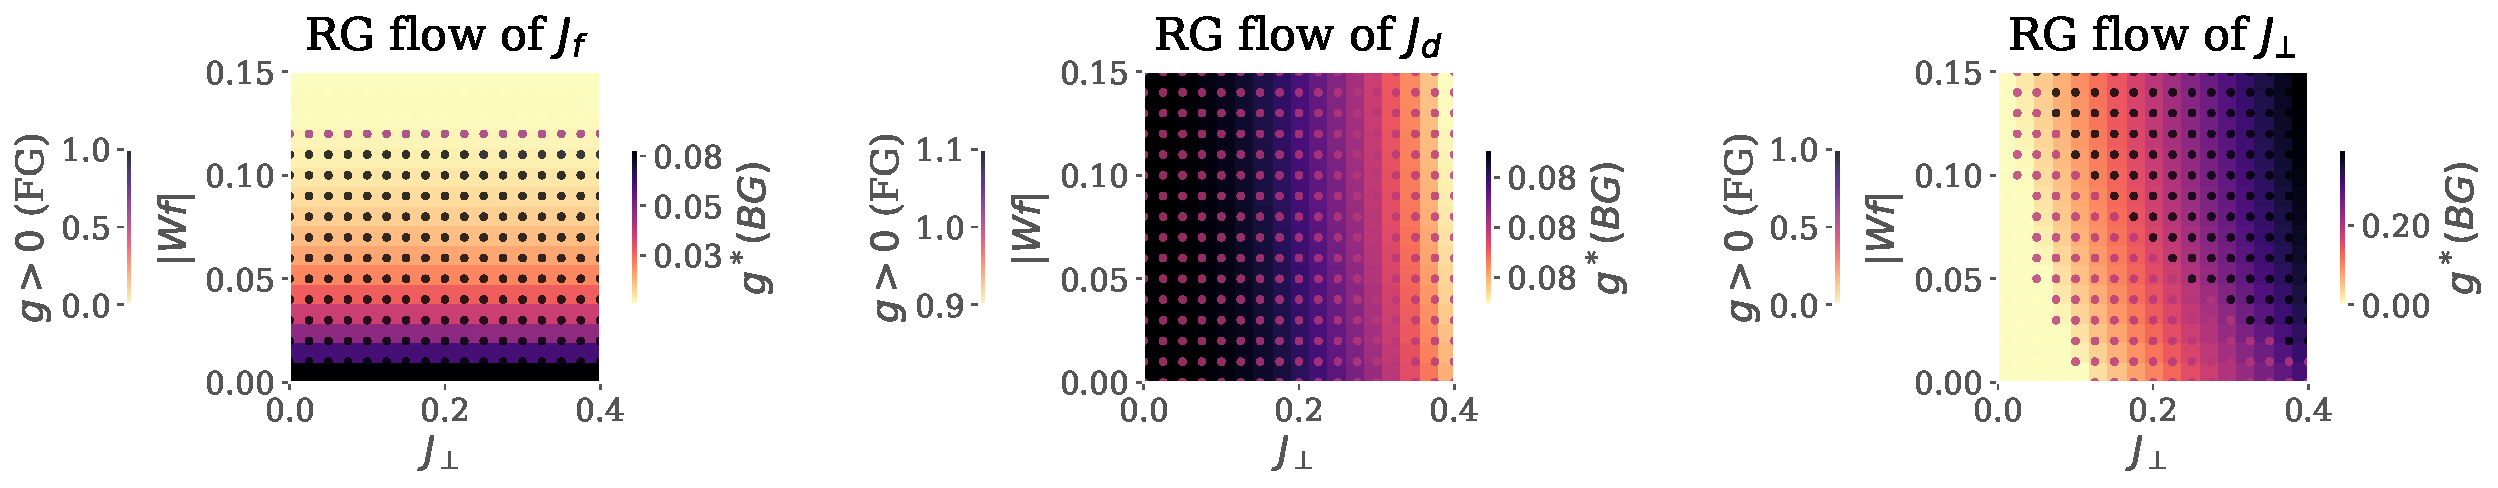
\includegraphics[width=\textwidth]{PD_33.pdf}
	\caption{RG phase diagrams for various Kondo couplings: \(f-\)layer (left), \(d-\)layer (middle) and inter-layer (right). For each plot, the background color (quantified by the right colorbar) tracks the fixed point value of the coupling as a function of the inter-layer couplings \(J_\perp\) and the \(f-\)layer bath interaction \(|W_f|\). The marker color complements this by tracking whether the coupling is relevant, intermediate-coupling or irrelevant in the RG sense, by taking the values 1, \(1/2\) or 0 respectively.}
	\label{couplingRG}
\end{figure}
We first analyse the model by obtaining unitary RG flows of three kinds of Kondo couplings. Fig.~\ref{couplingRG} shows the fixed point values of the couplings under renormalisation to a low-energy theory. We view these values as a function of the \(f-\)layer bath interaction \(W_f\) and inter-layer Kondo coupling \(J_\perp\). In each panel, the right (left) colorbar quantifies the background (marker) color of the plot. The background displays the fixed point value of each coupling whereas the marker color tracks whether the couplings is relevant (1), intermediate coupling (0.5) or irrelevant (0). 

The Kondo coupling \(J_d\) (middle panel) of the \(d-\)layer remains relevant for the entirety of the chosen parameter regime. The Kondo coupling \(J_f\) (left panel) of the \(f-\)layer becomes RG-irrelevant for larger values of \(|W_f|\); this leads to an in-plane Mott transition of the kind observed in our earlier work, where the local Fermi liquid excitations of the \(f-\)impurity give way to a pseudogapped non-Fermi liquid Mott metal phase which ultimately destabilises into a local moment phase. The RG flow of \(J_f\) does not appear to be significantly affected by the variation of \(J_\perp\). Concomitant with the irrelevance of \(J_f\) under increasing \(|W_f|\), the inter-plane coupling \(J_\perp\) (right panel) becomes RG-relevant, as seen from the darkening markers as we go to higher \(|W_f|\). 

These simulations motivate an RG-based phase diagram with the following regimes: (i) weak \(J_\perp\), weak \(|W_f|\): decoupled metallic layers, each layer participating in transport independently, (ii) strong \(J_\perp\), strong \(|W_f|\): Kondo insulator regime, where the local moments of the \(f-\)layer hybridise with the itinerant electrons of the \(d-\)layer to form a band insulator with the chemical potential situated in the hybridisation gap, and (iii) weak \(J_\perp\), strong \(|W_f|\): the so-called RKKY regime, where the \(f-\)layer forms local moments which decouple from the \(d-\)layer and are then free to order magnetically, and (iv) strong \(J_\perp\), weak \(|W_f|\): this is similar to the Kondo insulator regime, except here the \(f-\)electrons remain itinerant and it is they who hybridise with the \(d-\)electrons to again form two bands separated by a hybridisation gap.

\section{Results at half-filling}
\begin{figure}[!h]
	\centering
	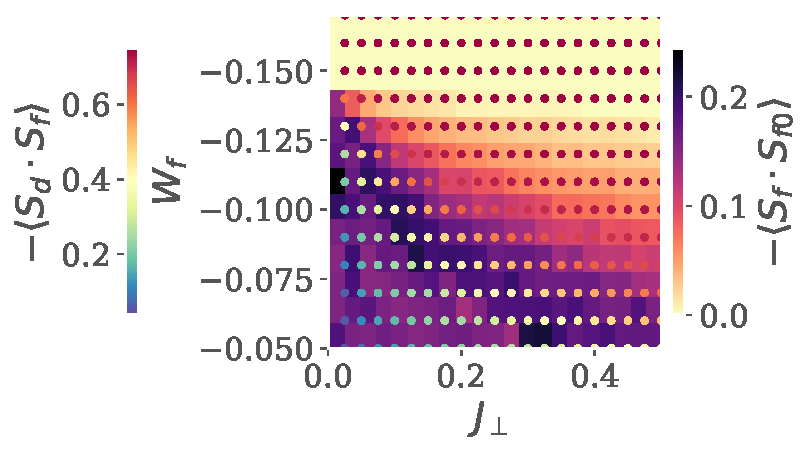
\includegraphics[width=0.4\textwidth]{locCorr_33_1299.pdf}
	\caption{Left: Real-space spin correlations for the auxiliary model. Background colour (right colourbar) represents that between the \(f-\)impurity and its nearest-neighbour sites, while the marker colour (left colourbar) represents that between the \(f-\)impurity and the \(d-\)impurity. While the former shrinks as \(J_\perp\) or \(|W_f|\) is increased, the latter grows. This marks a transfer of entanglement from intra-plane channel into inter-plane channel. Right: }
\end{figure}

\begin{figure}[!h]
	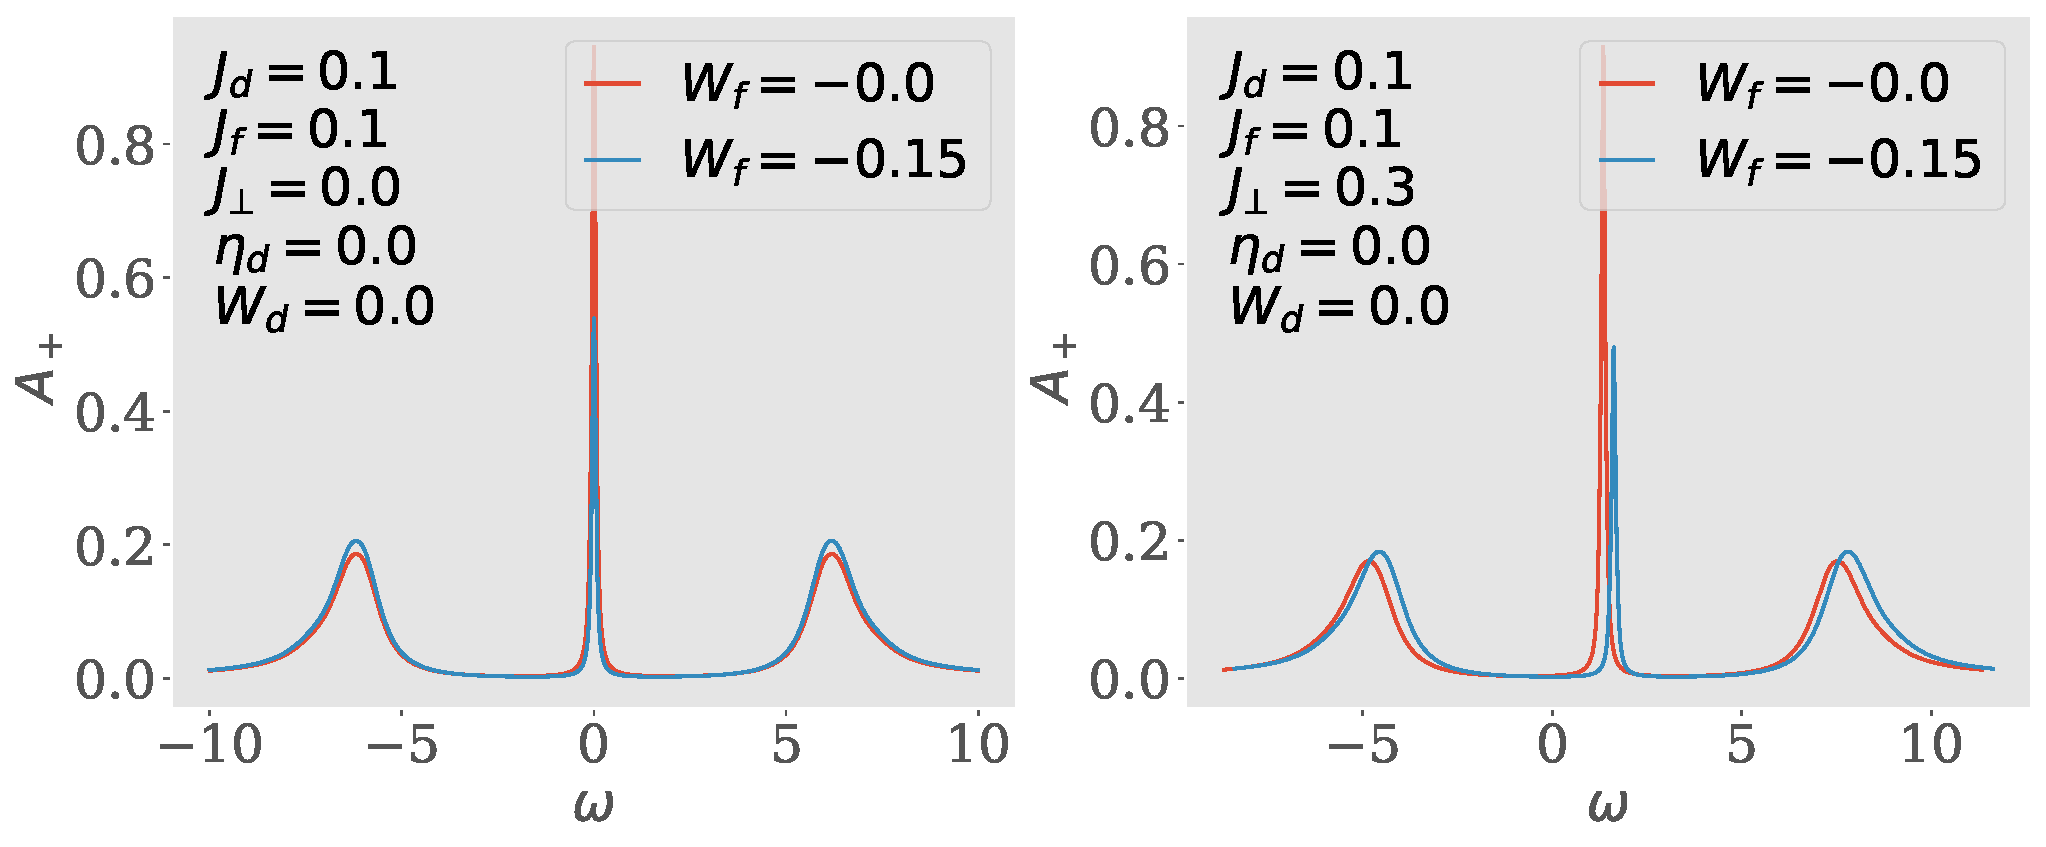
\includegraphics[width=0.49\textwidth]{specFunc_node_+_33_1555.pdf}
	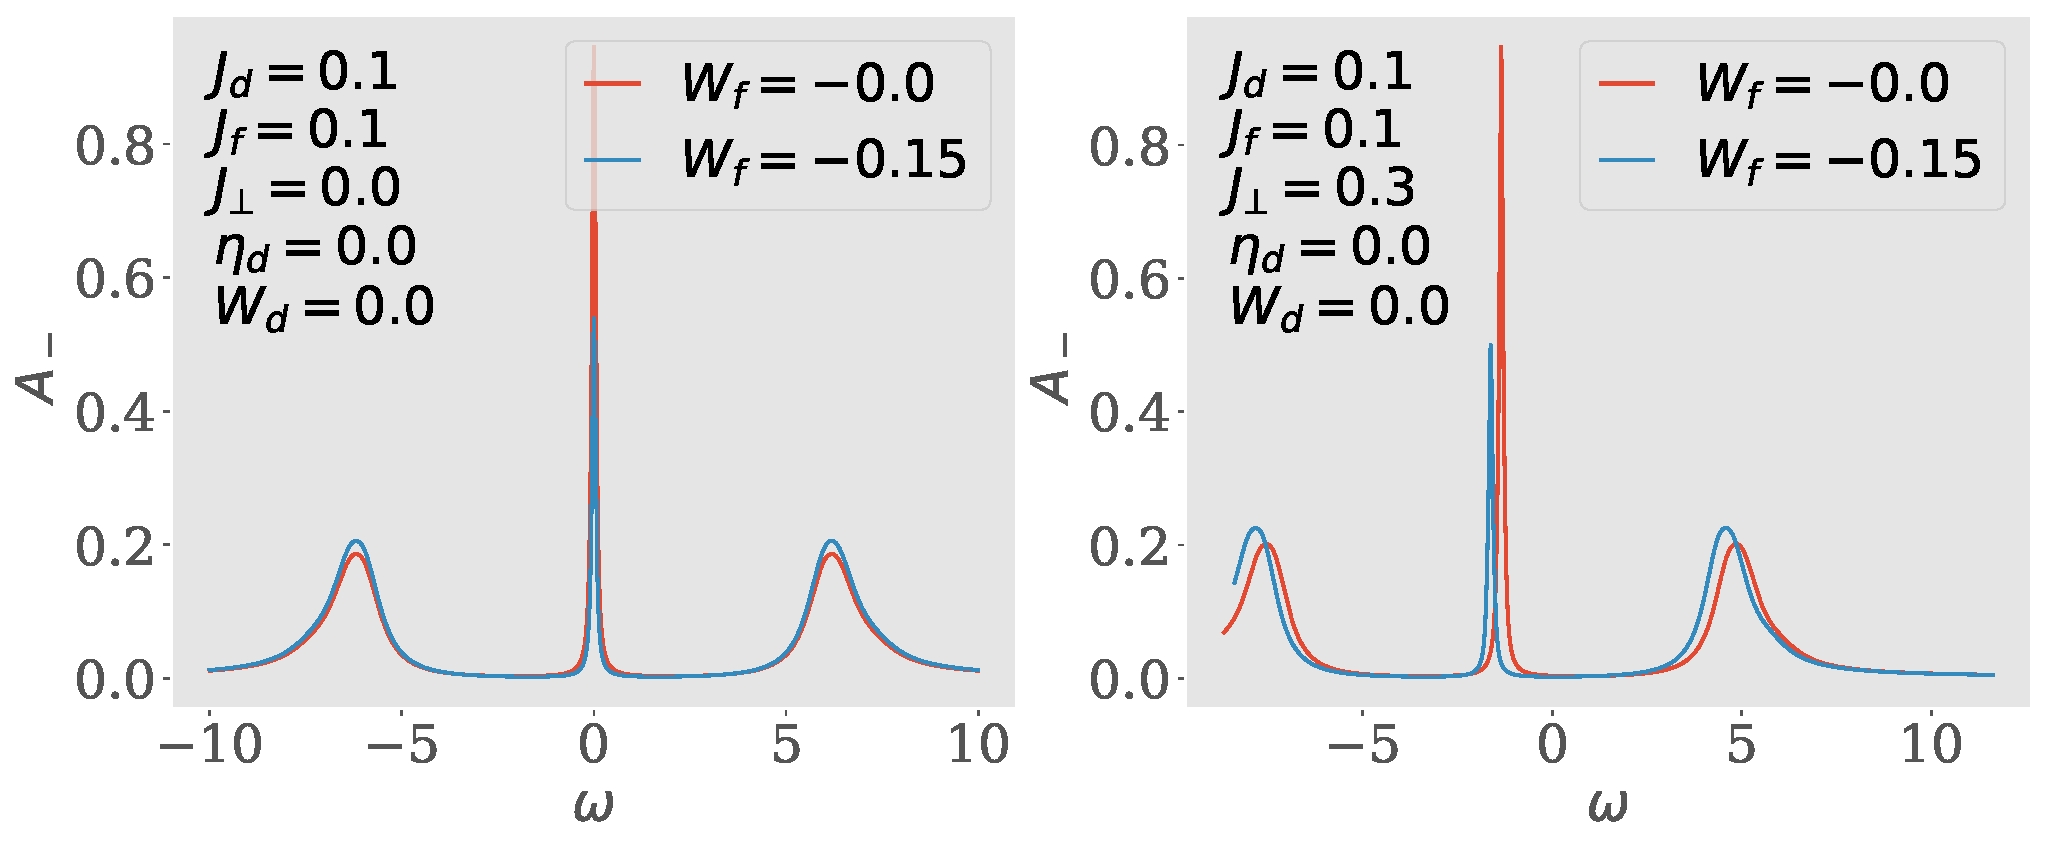
\includegraphics[width=0.49\textwidth]{specFunc_node_-_33_1555.pdf}
		\caption{Spectral functions of the tiled model, for excitations in the bonding (two on the left) and antibonding (two on the right) basis, defined by the Greens function \(G_{k,\pm} = G(k_d \pm k_f; \omega)\). There is no hybridisation for \(J_\perp=0\) (first and third plots), and the only effect of \(W_f\) is to shrink the height of the central resonance. Introducing a non-zero \(J_\perp\) splits the central resonance into an upper band (second from left) and a lower band (first from right). This leads to a Kondo insulator, where \(\omega=0\) resides inside the hybridisation gap.
		}
\end{figure}

\begin{figure}[!h]
	\centering
	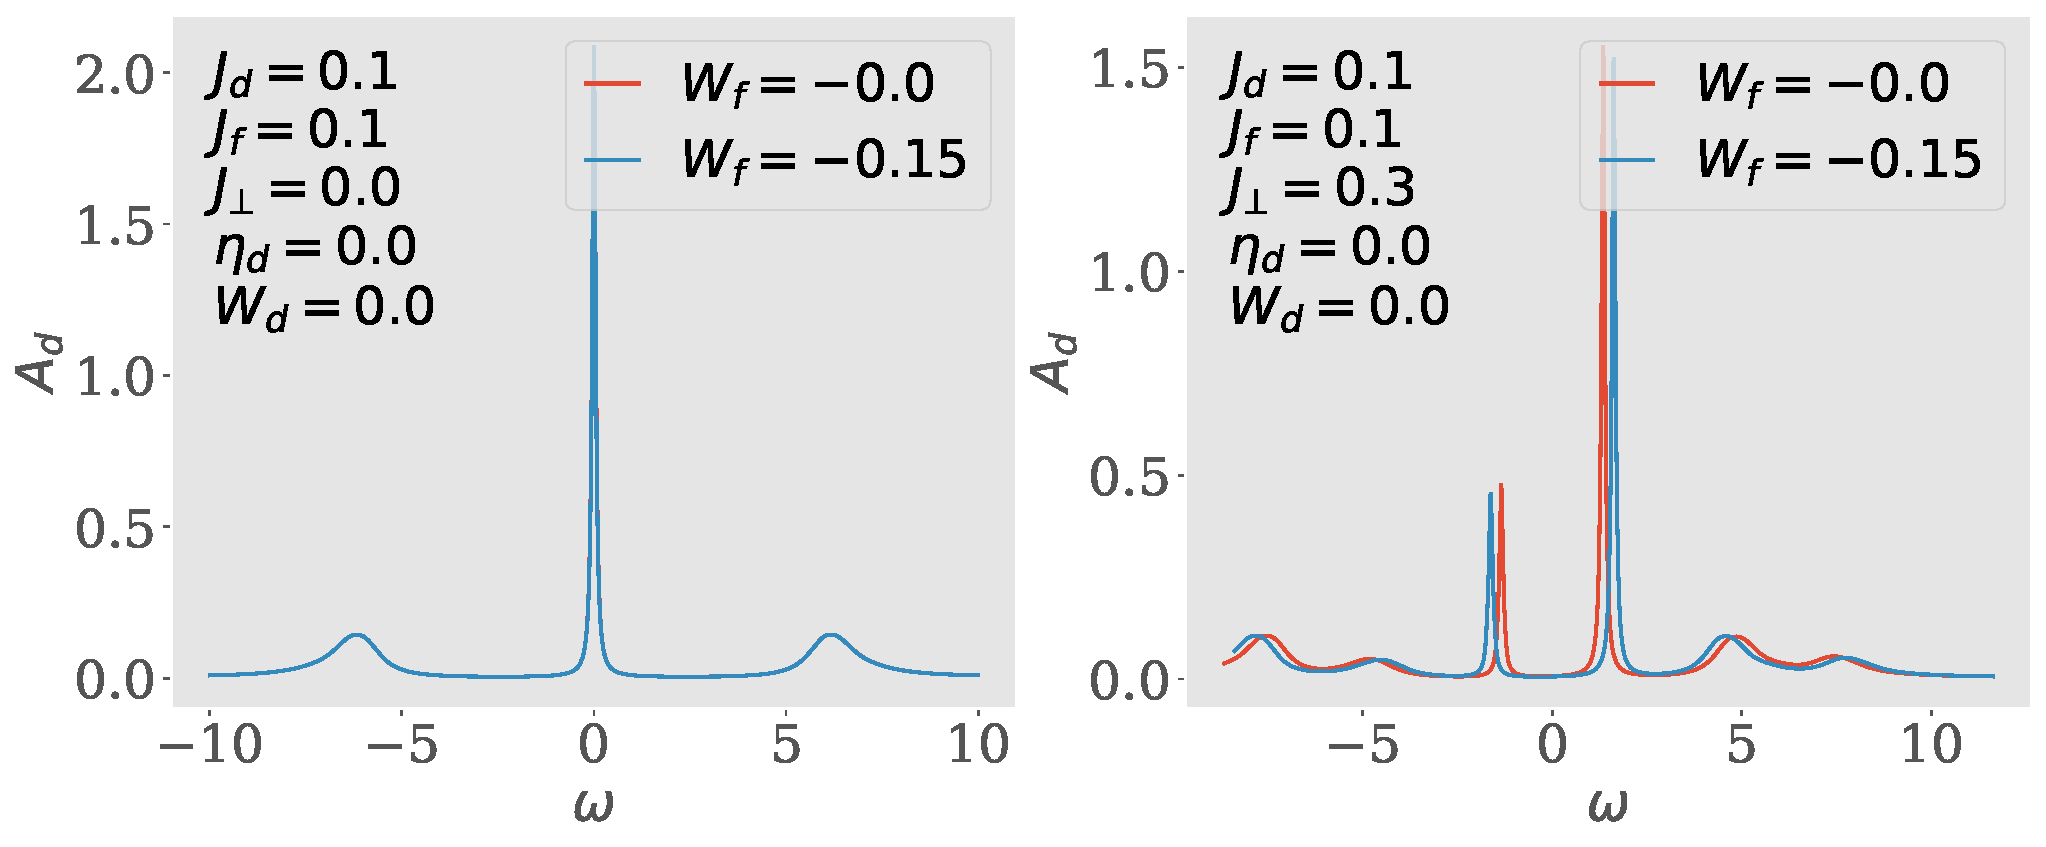
\includegraphics[width=0.49\textwidth]{specFunc_node_d_33_1555.pdf}
	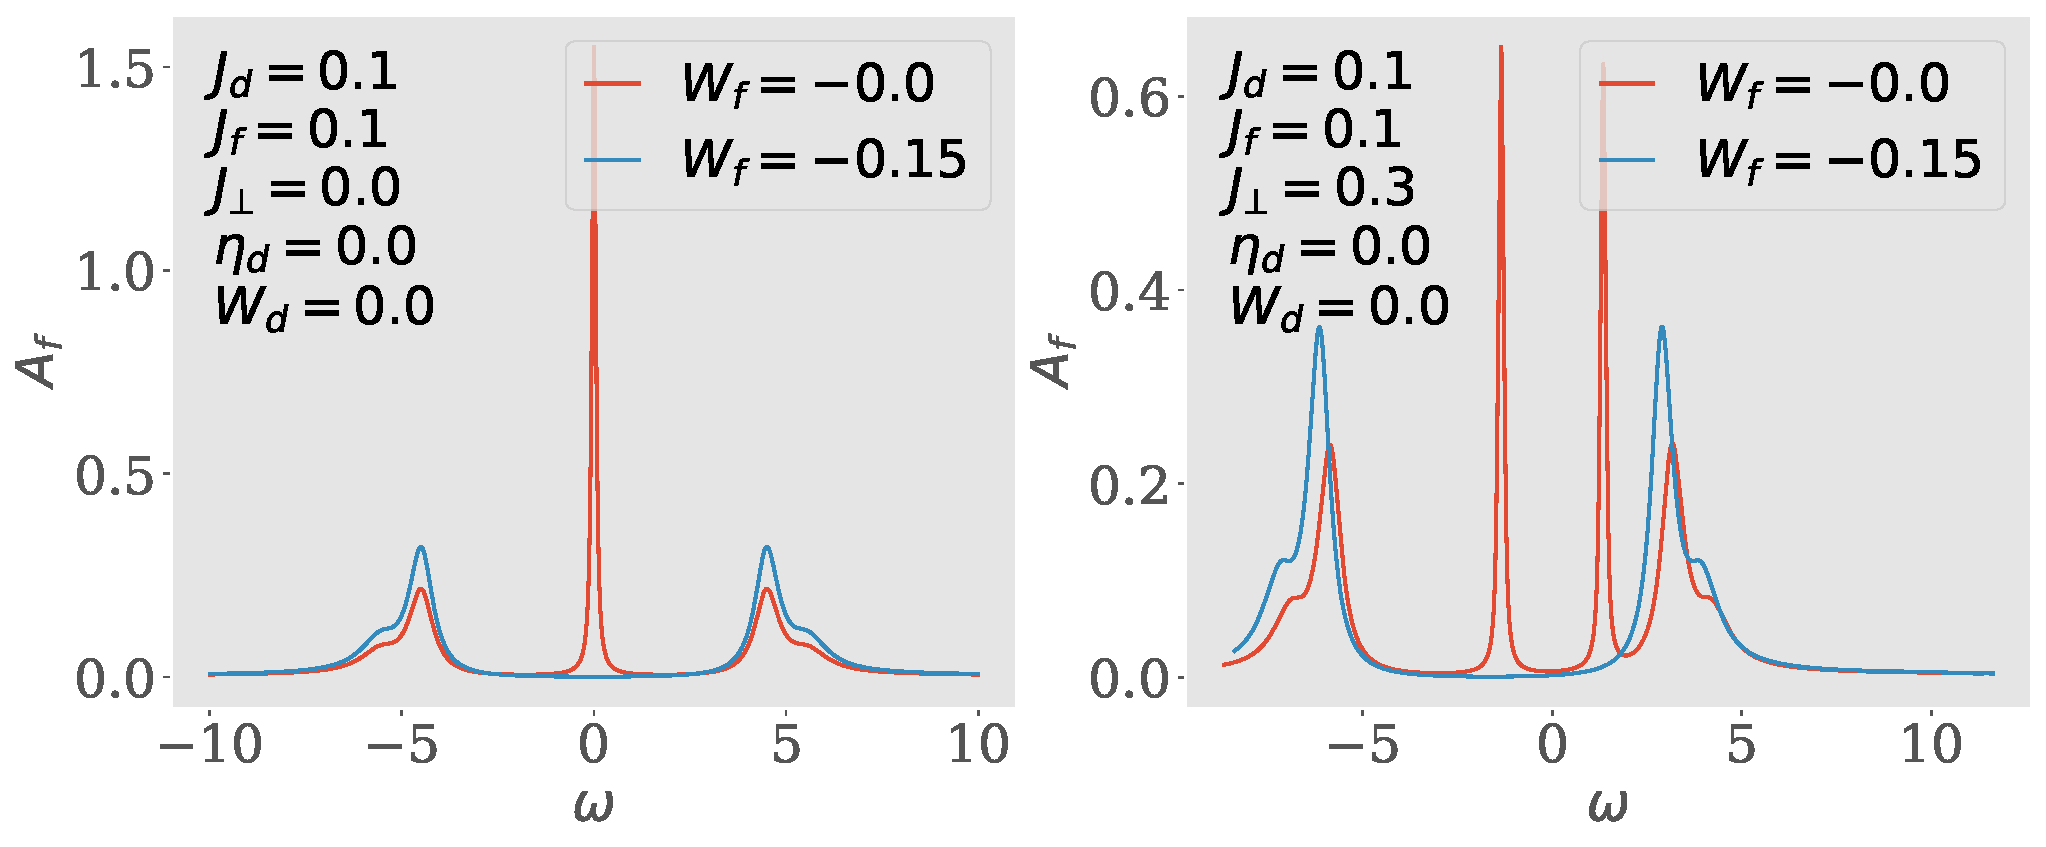
\includegraphics[width=0.49\textwidth]{specFunc_node_f_33_1555.pdf}
	\caption{Spectral functions \(A_d\) and \(A_f\) of the auxiliary model, for excitations in the \(d-\) and \(f-\)layers respectively. Both show a central Kondo resonance for \(J_\perp=0\) which splits into two bands upon adding a non-zero \(J_\perp\). Increasing \(|W_f|\) to large values gaps out the local Fermi liquid excitations of \(A_f\).
	}
\end{figure}

% \include{metalsRG/metalsRG.tex}
% \chapter{\chapH}
In the final chapter, we will summarise the results obtained from the research carried out in the thesis, clarify the major conclusions derived from them, and point out some avenues for further work. In a nutshell, we have applied a two-pronged approach to metal-insulator transitions through this body of work. The first approach tackles the effects of strong local correlation through the development of a new method that maps interacting fermionic models to quantum impurity models. The other complimentary approach involves studying the effects of metal-insulator transition on entanglement renormalisation, and characterising phases through the emergent geometry resulting from such flows.

% \include{appendices/appendices.tex}

\bibliography{thesis_cleaned}
\bibliographystyle{unsrt}
\end{document}

%%%%%%%% TODO
%% Page numbers at bottom
%% Truncate headers perhaps
%% Fix \Delta V Rg equation and derivation
%% Add reference to published papers along with Stoyanova thesis and use the papers to improve the discussion of many Bloch's theorem
%% rectify incorrect description below definition of impurity-bath T operator (c + S + C) c_k
%% glue between chapters, improve beginning of each chapter before work sections
%% finalise methods chapter
%% remove repeated stuff on auxiliary models from tiling/mott metal chapter
%% check out the expression for G_local in tiling formalism, seems like it's incorrect (it appears to be missing the G(r_d, r) contributions
%% Add renormalised perturbation theory to methods
%% Fix star graph URG in methods
%% Add description of tiling method into introduction (motivation, features)
%% Add some of the picture I created for the presub presentation
